% XeLaTeX can use any Mac OS X font. See the setromanfont command below.
% Input to XeLaTeX is full Unicode, so Unicode characters can be typed directly into the source.

% The next lines tell TeXShop to typeset with xelatex, and to open and save the source with Unicode encoding.

%!TEX TS-program = xelatex
%!TEX encoding = UTF-8 Unicode

\documentclass[12pt,twoside]{book}

\usepackage{geometry}                % See geometry.pdf to learn the layout options. There are lots.
\geometry{a4paper}                   % ... or a4paper or a5paper or ... 
%\geometry{landscape}                % Activate for for rotated page geometry
%\usepackage[parfill]{parskip}    % Activate to begin paragraphs with an empty line rather than an indent
\usepackage{amssymb}
\usepackage{todonotes}
\usepackage{booktabs}
\usepackage{longtable}


% Will Robertson's fontspec.sty can be used to simplify font choices.
% To experiment, open /Applications/Font Book to examine the fonts provided on Mac OS X,
% and change "Hoefler Text" to any of these choices.

\usepackage{fontspec,xltxtra,xunicode}
\defaultfontfeatures{Mapping=tex-text}
\setromanfont[Mapping=tex-text]{Optima}
\setsansfont[Scale=MatchLowercase,Mapping=tex-text]{Optima}
\setmonofont[Scale=MatchLowercase]{Andale Mono}

%%%% Graphics
\usepackage{graphicx}
\usepackage{tikz}
\definecolor{unilublue}{RGB}{55,149,218}
\definecolor{sntred}{RGB}{219,46,27}
\definecolor{sntpurple}{RGB}{86,30,130}
%\definecolor{sntblue}{RGB}{50,130,207}
\definecolor{sntblue}{RGB}{55,149,218}

\pgfdeclareimage[width=30mm]{logo-snt}{logos/logo-snt}
\pgfdeclareimage[width=30mm]{logo-uni-lu}{logos/logo-uni-lu}

%%%% Fancy
\usepackage{fancyhdr}

%%%% Increase page length
\addtolength{\textheight}{1in}

%%%% Sections
\usepackage{sectsty}
\allsectionsfont{\sffamily}

%%%% Title
\newcommand{\titleone}{\textsf{Fault-based Automated Quality Assurance of Test Suites:}}
\newcommand{\titletwo}{\textsf{Practical Mutation Testing for Satellite and Embedded Systems}}

\newcommand{\todoinline}[1]{\todo[color=orange,inline]{ \textbf{Note}: #1 }}



\newcommand{\OffuttADA}{\cite{rothermel1996experimental}}
\newcommand{\MUSIC}{\cite{phan2018music}}
\newcommand{\Sciror}{\cite{hariri2018srciror}}
\newcommand{\Mull}{\cite{denisov2018mull}}
\newcommand{\Accmut}{\cite{wang2017faster}}
\newcommand{\Major}{\cite{just2014major}}
\newcommand{\MuJava}{\cite{ma2006mujava}}
\newcommand{\TuyaSQL}{\cite{tuya2007mutating}}
\newcommand{\BinhSimulink}{\cite{binh2012mutation}}
\newcommand{\Proteum}{\cite{delamaro2001interface}}
\newcommand{\Shahriar}{\cite{shahriar2008mutation}} % not a tool 
\newcommand{\SMT}{\cite{dan2012semantic}}
\newcommand{\MUSICShahriar}{\cite{shahriar2008music}}
\newcommand{\MuCPP}{\cite{delgado2017assessment}}
\newcommand{\jMINT}{\cite{grechanik2016mutation}}
\newcommand{\ILMutator}{\cite{derezinska2011object}}
\newcommand{\SQLChan}{\cite{chan2005fault}}
\newcommand{\BacterioSystem}{\cite{mateo2012validating}}
\newcommand{\Milu}{\cite{jia2008milu}}
\newcommand{\Judy}{\cite{madeyski2010judy}}



\begin{document}

\pagestyle{fancy}
\renewcommand{\sectionmark}[1]{\markright{\textit{#1}}}

\renewcommand{\headrulewidth}{2pt}% 2pt header rule
\renewcommand{\headrule}{\hbox to\headwidth{%
  \color{sntblue}\leaders\hrule height \headrulewidth\hfill}}

\fancyhf{}

%\lhead{\fancyplain{}{\setlength{\unitlength}{1mm}
%\begin{picture}(0,0)
%\put(0,-4){
\includegraphics[width=50pt]{logos/logo-snt}}
%\end{picture}}} 

\lhead{\fancyplain{}{\textit{Mutation Testing Survey}}}

\rhead{\fancyplain{}{\rightmark }}

\fancyfoot[C]{%
\begin{tikzpicture}[remember picture,overlay]
\path [fill=sntred]    ([xshift=88pt,yshift=20pt]current page.south west) rectangle
                       ([xshift=229pt,yshift=50pt] current page.south west);
\path [fill=sntpurple] ([xshift=229pt,yshift=20pt] current page.south west) rectangle
                       ([xshift=370pt,yshift=50pt] current page.south west);
\path [fill=sntblue]   ([xshift=370pt,yshift=20pt] current page.south west) rectangle
                       ([xshift=510pt,yshift=50pt] current page.south west);
\end{tikzpicture}
}

\fancyfoot[RO]{
\begin{tikzpicture}[remember picture,overlay]
\node [circle, ultra thick, fill=white, draw=sntblue] at ([xshift=530pt,yshift=35pt] current page.south west) {\thepage};
\end{tikzpicture}}

\fancyfoot[LE]{
\begin{tikzpicture}[remember picture,overlay]
\node [circle, ultra thick, fill=white, draw=sntblue] at ([xshift=65pt,yshift=35pt] current page.south west) {\thepage};
\end{tikzpicture}}


\newcommand{\CHANGED}[1]{\textcolor{blue}{#1}}

\thispagestyle{empty}

\begin{tikzpicture}[remember picture,overlay]
\path [fill=sntred]    ([xshift=30pt,yshift=20pt]current page.south west) rectangle
                       ([xshift=210pt,yshift=50pt] current page.south west);
\path [fill=sntpurple] ([xshift=210pt,yshift=20pt] current page.south west) rectangle
                       ([xshift=390pt,yshift=50pt] current page.south west);
\path [fill=sntblue]   ([xshift=390pt,yshift=20pt] current page.south west) rectangle
                       ([xshift=570pt,yshift=51pt] current page.south west);
\path [fill=unilublue] ([xshift=30pt,yshift= 50pt] current page.south west) --
                       ([xshift=570pt,yshift= 50pt] current page.south west)
                       [rounded corners=20pt] --
                       ([xshift=570pt,yshift=740pt] current page.south west)
                       [sharp corners] --
                       ([xshift=30pt,yshift=740pt] current page.south west);
\node [fill=white,rounded corners=0pt,inner xsep=6pt,inner ysep=3pt]
      at ([xshift=523pt,yshift=120pt] current page.south west)
      {\pgfuseimage{logo-uni-lu}};

\node [fill=white,rounded corners=2pt,inner xsep=6pt,inner ysep=3pt]
      at ([xshift=520pt,yshift=780pt] current page.south west)
      {\pgfuseimage{logo-snt}};

%\node [circle, fill=white, draw=sntblue] at ([xshift=550pt,yshift=35pt] current page.south west) {a};

\node[draw=none,fill=none,right] at (-1, -7){\color{white}\LARGE\bf\titleone};
\node[draw=none,fill=none,right] at (-1, -8){\color{white}\LARGE\bf\titletwo};
\node[draw=none,fill=none,right] at (-1, -9){\color{white}\LARGE\bf\titlethree};

\node[draw=none,fill=none,right] at (-1, -12){\color{white}\Large\textsf{O. Cornejo, F. Pastore, E. Viganò}};
\node[draw=none,fill=none,right] at (-1, -13){\color{white}\Large\textsf{Interdisciplinary Centre for Security, Reliability and Trust}};
\node[draw=none,fill=none,right] at (-1, -14){\color{white}\Large\textsf{University of Luxembourg}};
\node[draw=none,fill=none,right] at (11, -16){\color{white}\textsf{ITT-1-9873-ESA-FAQAS-SUTP}};
\node[draw=none,fill=none,right] at (11, -17){\color{white}\Large\textsf{Issue 4, Rev. 1}};
\node[draw=none,fill=none,right] at (11, -18){\color{white}\Large\textsf{\today}};
\node[draw=none,fill=none,right] at (-1, -24){\color{white}\tiny\textsf{EUROPEAN SPACE AGENCY. CONTRACT REPORT.}};
\node[draw=none,fill=none,right] at (-1, -24.3){\color{white}\tiny\textsf{The work described in this report was done under ESA contract. Responsibility for the contents resides in the author or organisation that prepared it.}};
\node[draw=none,fill=none,right] at (-1, -24.8){\color{white}\tiny\textsf{The copyright in this document is vested in the University of Luxembourg.}};
\node[draw=none,fill=none,right] at (-1, -25.1){\color{white}\tiny\textsf{This document may only be reproduced in whole or in part, or stored in a retrieval system,or transmitted in any form, or by any means electronic,}};
\node[draw=none,fill=none,right] at (-1, -25.4){\color{white}\tiny\textsf{mechanical, photocopying or otherwise, either with the prior permission of the University of Luxembourg or in accordance with the terms of ESTEC Contract No. 4000128969/19/NL/AS.}};

\node[draw=none,fill=none,right] at (-1, -24){\color{white}\tiny\textsf{EUROPEAN SPACE AGENCY. CONTRACT REPORT.}}; 
\node[draw=none,fill=none,right] at (-1, -24.3){\color{white}\tiny\textsf{The work described in this report was done under ESA contract. Responsibility for the contents resides in the author or organisation that prepared it.}};
\node[draw=none,fill=none,right] at (-1, -24.8){\color{white}\tiny\textsf{The copyright in this document is vested in the University of Luxembourg.}};
\node[draw=none,fill=none,right] at (-1, -25.1){\color{white}\tiny\textsf{This document may only be reproduced in whole or in part, or stored in a retrieval system,or transmitted in any form, or by any means electronic,}}; 
\node[draw=none,fill=none,right] at (-1, -25.4){\color{white}\tiny\textsf{mechanical, photocopying or otherwise, either with the prior permission of the University of Luxembourg or in accordance with the terms of ESTEC Contract No. 4000128969/19/NL/AS.}};


\end{tikzpicture}

\newpage


% !TEX root = MAIN.tex

\chapter{Scope and content}

This document is the deliverable SSS of the ESA activity ITT-1-9873-ESA. It concerns requirements specification for the \emph{FAQAS framework} to be delivered by ITT-1-9873-ESA. Following the structure described in the SoW \emph{AO9873-ws00pe\_SOW.pdf}, it provides the structured requirements baseline for the FAQAS framework according to ECSS-E-ST-40C Annex B.
 
\section{Applicable and reference documents}

\begin{itemize}
\item{D1 - Mutation testing survey}
\item{D2 - Study of mutation testing applicability to space software}
\end{itemize}

\chapter{Terms, definitions and abbreviated terms}

\begin{itemize}
\item{FAQAS}: activity ITT-1-9873-ESA
\item{FAQAS-framework}: software system to be released at the end of WP4 of FAQAS
\item{D2}: Deliverable D2 of FAQAS, \emph{Study of mutation testing applicability to space software}
\item{KLEE}: Third party test generation tool, details are provided in D2.
\item{SUT}: Software under test, i.e, the software that should be mutated by means of mutation testing.
\item{WP}: Work package
\end{itemize}

\clearpage
 



% !TEX root = MAIN.tex

\chapter{Code-driven Mutation Testing}
\label{chapter:codemutation}

% !TEX root = MutationTestingSurvey.tex

\section{Mutation Testing Process}
\label{sec:process}

	\begin{figure}
	\centering
		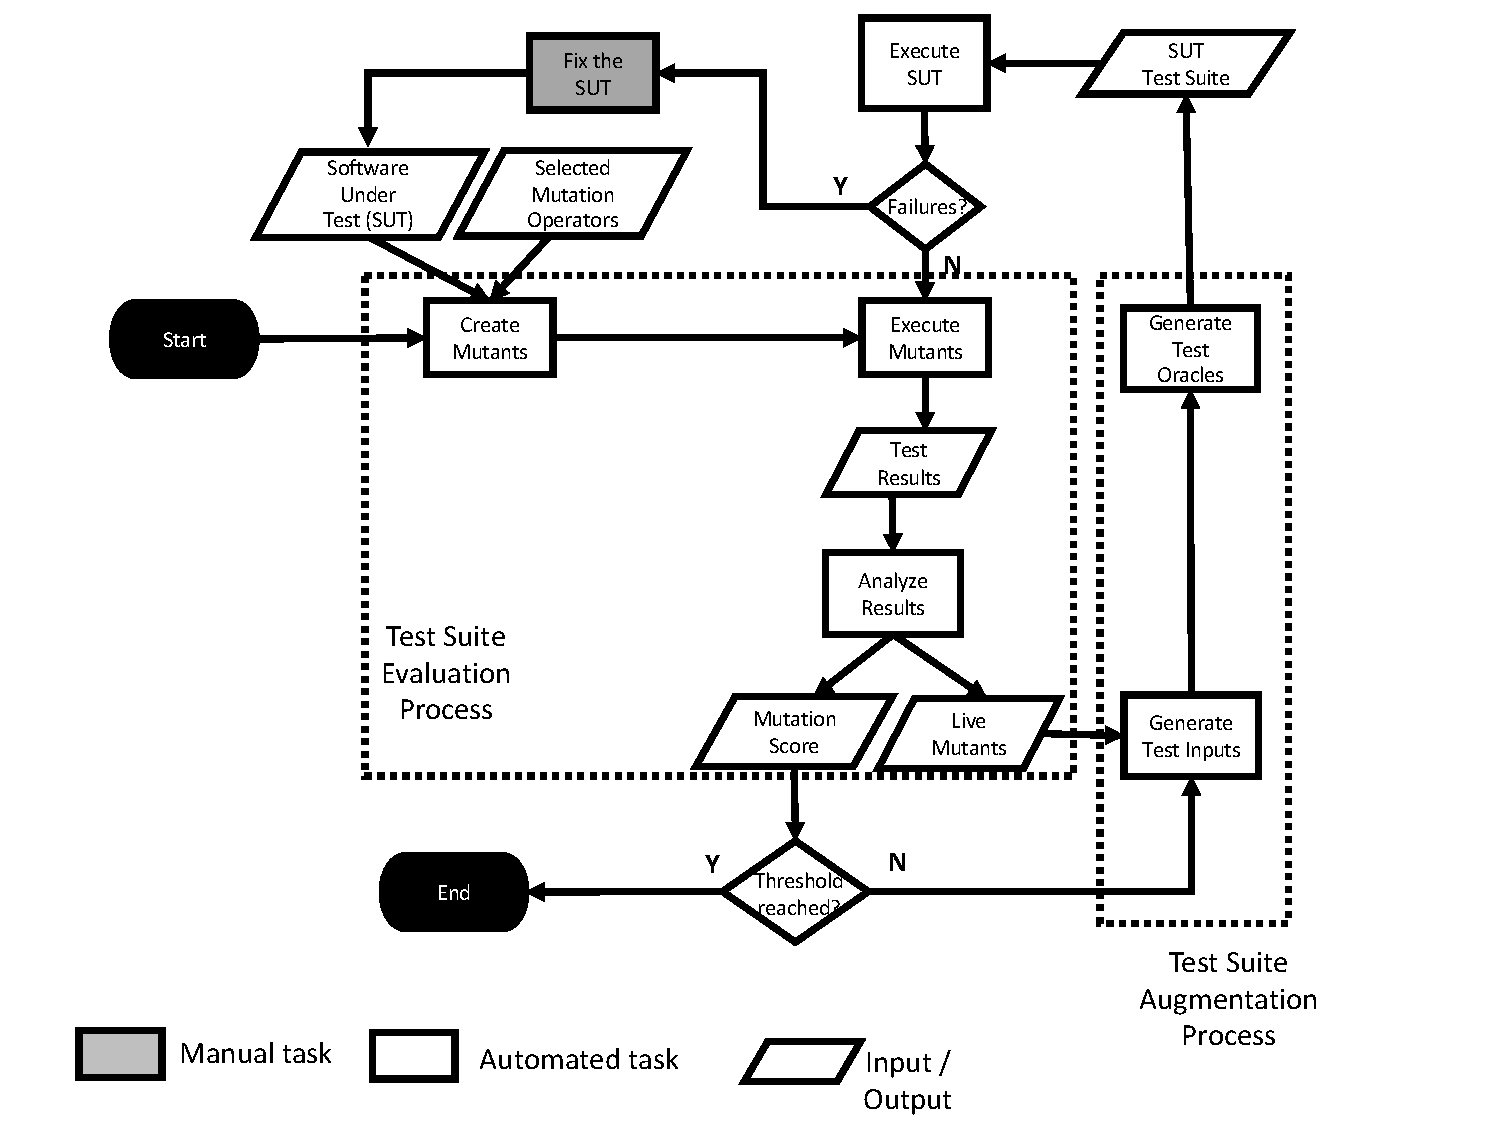
\includegraphics[width=\textwidth]{images/process}
		\caption{Mutation Testing Process.}
		\label{fig:code:process}
	\end{figure}

Figure \ref{fig:code:process} shows the reference code-driven mutation testing process that will be considered in this book. The process depicted in Figure \ref{fig:code:process} has been inspired by the mutation testing process described in related work \cite{offutt2001mutation,papadakis2019mutation}. The process is based on two main sub-processes, \emph{test suite evaluation} and \emph{test suite augmentation}, which are described in Sections~\ref{sub:test_suite_evaluation}~and~\ref{sub:test_suite_augmentation}, respectively.


\subsection{Test Suite Evaluation} % (fold)
\label{sub:test_suite_evaluation}

The Test Suite Evaluation process concerns the automatic generation of modified versions (i.e., the mutants) of the software under test (SUT) and the evaluation of the quality of the SUT test suite. It consists of three activities: \emph{create mutants}, \emph{execute mutants}, and \emph{analyze results}. 
These activities are typically automated by toolsets that often include strategies to address scalability issues. 

Figure~\ref{fig:code:process} provides an overview of the test suite evaluation process.
It starts with engineers providing the SUT and a set of mutation operators selected to be considered for creating modified versions of the software. 
The set of available mutation operators depends on the toolset implementing the test suite evaluation process. 
A set of mutation operators implemented by most of the existing toolsets consists of the relational (ROR), logical (LCR), arithmetic (AOR), absolute (ABS) and unary insertion (UOI) operators \cite{rothermel1996experimental}. 
%Several research paper target the definition of mutation operators; relevant for this ESA activity are works on the definition of mutants for floating point operators \cite{dan2012semantic}, operators synthesized by processing the revision history of C projects \cite{brown2017care}, mutation operators targeting memory operations \cite{wu2017memory}, deletion operators \cite{delamaro2014designing}, operators targeting components integration \cite{grechanik2016mutation}. Finally, recent attention has been put towards the development of higher-order mutation operators \cite{harman2010manifesto,ghiduk2017higher}. First order mutation seeds faults generated by a single syntactic change to the original program. Higher order mutation combines first order mutants to simulate more complex faults, motivated by a desire to capture subtle faults \cite{jia2009higher}. 
Section~\ref{sec:operators} provides an overview of the mutation operators defined in the literature that can be applied in the context of space and embedded systems.

In the test suite evaluation process, the activity \emph{create mutants} concerns the application of the mutation operators to the source code of the SUT; it leads to the generation of modified versions of the SUT (i.e., the mutants) that should be compiled and then executed against the test suite to evaluate the test suite quality. 
The \emph{execution of mutants} implies the execution of the test suite of the SUT against all the generated mutants. 
%Optimizations for the execution of mutants concern the scalability of the execution process and 
%the identification at run-time of equivalent and redundant mutants.

Unfortunately, the activity \emph{create mutants} leads to a high number of mutants to be generated, which, in turn, leads to scalability issues due to the compilation and execution of the different program versions generated. Recent surveys provide an overview of existing optimization techniques~\cite{ferrari2018systematic};
the most relevant optimization approaches target the reduction of the number of mutants to be compiled and executed, 
the reduction of the compilation iterations, the reduction of the execution time, and the identification of equivalent and redundant mutants.

To reduce the number of program versions that need to be compiled and executed, existing approaches automatically select subsets of the generated mutants. Two main mutant selection approaches have been defined: the selection of representative mutation operators and the random selection of mutants \cite{zhang2010operator}. The first approach consists of the empirical identification of a subset of mutation operators that is sufficient to predict the mutation score \cite{siami2008sufficient,barbosa2001toward}. The second approach consists of randomly selecting a certain percentage of mutants from the generated ones \cite{wong1995reducing}, possibly with a uniform distribution of the different mutation operators \cite{zhang2010operator}. Empirical results with academic case studies \cite{zhang2010operator} show that the first approach is not superior to random selection when selecting the same number of mutants. Other work \cite{zhang2013operator} show that the combination of operator-based selection and random sampling leads to better results since it leads to high mutation score (above 98\%) while reducing the average mutation testing time to 6.54\%. The use of higher-order mutants is another solution to reduce the overall number of mutants. 
Other optimizations are framework specific, for example, Mull limits mutations to reachable code \cite{hariri2018srciror}. Section~\ref{sec:opt:selection} provides an overview of mutant selection approaches.

To reduce the time spent in the compilation of the generated mutants, mutant schemata \cite{untch1993mutation} consist of encoding all the mutants in a single file and parametrize the mutant execution so that mutants are compiled in a single pass and selected at runtime. Section~\ref{sub:compileTime} provides an overview of compile-time optimization approaches.

Another optimization that speeds up the compilation of mutants concerns the identification of equivalent and redundant mutants. Equivalent mutants are mutants that behave as the original program, while redundant mutants are mutants that lead to the same test failures. 
To detect if a program and one of its mutants are
equivalent is undecidable~\cite{Budd:1982}; however, heuristics to partially address the problems have been defined in the literature.
Trivial compiler optimization might be adopted to detect both equivalent and redundant mutants; it relies on the idea that source code that leads to the same program behaviour often belongs to the same optimized compiled code \cite{papadakis2015trivial}. Other approaches concern the adoption of symbolic execution \cite{papadakis2012mutation,kurtz2015static} and the runtime monitoring of the SUT (e.g., mutants that lead to the same execution paths are likely equivalent \cite{schuler2013covering}). Finally, Shin et al. proposed the \emph{distinguishing mutation adequacy criterion}, which aims to ensure that the test suite includes enough different test inputs so that every mutant is distinguished by each other, if feasible~\cite{shin2017theoretical}. 
Solutions to address the problem of identifying equivalent and redundant mutants are detailed in Sections~\ref{sec:opt:equivalent} and~\ref{sec:opt:redundant}, respectively.






A well-known optimization to \emph{reduce execution time} is the split-stream optimization, which consists of generating a modified version of the SUT that creates multiple processes (one for each mutant) only when the mutated code is reached \cite{tokumoto2016muvm}. With split-stream, the code shared among multiple mutants is executed only once thus saving time and resources. Other execution optimizations consist of minimizing the number of processes being created by sharing one single process among mutants that bring the system into the same state \cite{wang2017faster}.
Section~\ref{sec:opt:execution} provides an overview of techniques to reduce execution time and, more generally, address run-time scalability issues.



The \emph{analysis of test results} concerns the identification of mutants that lead to the failure of at least one test case of the SUT test suite; these mutants are said to be \emph{killed}. Mutants that do not lead to the failure of any test case are said to be \emph{live mutants}. The identification of killed and live mutants enable the definition of a mutation adequacy criterion as follow, \emph{a test suite is mutation-adequate if all mutants are killed by at least one test of the test suite}. 
Also, the percentage of killed mutants is used to quantitatively measure the quality of a test suite. This measure is referred to as \emph{mutation score}.
Because of equivalent and redundant mutants, mutation-adequacy is difficult to achieve while the mutation score might not be representative of test suites quality~\cite{papadakis2016threats}. Section~\ref{sub:mutationscore} provides an overview of solutions addressing the problems related to the computation of the mutation score.



The capability of a test case to kill a mutant often depends on the observability of the system state. 
To overcome the limitations due to observability, different strategies for distinguishing program executions (i.e, to determine if the execution of two test cases led to different results) have been defined. These strategies are known as strong, weak, firm, and flexible mutation coverage.
\emph{Strong mutation coverage} indicates that the computation of the mutation score is based on the percentage of mutants identified by test failures, i.e., based on difference between the expected and the observed output of the system.  
\emph{Weak mutation coverage} consists of verifying if the state of the system has been altered, with respect to the original code, after the execution of the mutated statement. 
\emph{Firm mutation coverage} consists of verifying if the change in the state of the system propagates after the mutated code, e.g., at function boundaries. 
\emph{Flexible mutation coverage} consists of checking if the mutated code leads to object corruption \cite{mateo2012validating}. The main difference between these four coverage strategies is that only strong mutation coverage enables engineers to assess the quality of test cases in their entirety, i.e., by evaluating both the capability of triggering an erroneous behavior and the capability of reporting the erroneous behaviour thanks to complete test oracles. The other strategies only evaluate the capability of the test suites of triggering the erroneous behavior. 

% subsection test_suite_evaluation (end)

\subsection{Test Suite Augmentation} % (fold)
\label{sub:test_suite_augmentation}

The test suite augmentation process concerns the definition of test cases that kill live mutants.
It consists of four activities \emph{Identify Test Inputs}, \emph{Generate Test Oracles}, \emph{Execute the SUT}, \emph{Fix the SUT}. The first two activities concern the definition of new test cases.
The third activity, i.e., the execution of the SUT, enables engineers to determine if the newly defined test cases spot faults not identified by the original test suite. 
Finally, the repair of the SUT (i.e., activity \emph{Fix the SUT}) is performed in the case of test failures.
In this book we focus on the techniques that can be applied to automate the first two activities (i.e., \emph{Identify Test Inputs}, and \emph{Generate Test Oracles}).
 
The identification of test inputs has the objective of identifying inputs for the SUT that make the SUT produce an output that is different than the one produced by one of the mutants not killed by the existing test suite.
%To this end, mutants could be ranked according to their importance in order to ensure that, for a given test budget, the most relevant mutants are considered first. MuRanker \cite{namin2015muranker}, for example, ranks mutants according to their predicted difficulty and complexity in being detected. 
Existing work investigated the adoption of the KLEE symbolic execution engine \cite{holling2016nequivack} and the use of bounded model checking \cite{riener2011test}. Other work combines dynamic symbolic execution (DSE) with search-based software testing (SBST) to generate test inputs that lead to strong mutations \cite{harman2011strong}. 

The generation of test oracles, instead, should lead to the generation of executable code instructions (e.g., assertions) that verify if the output generated by the SUT is correct.
In the case of automated test generation approaches, a state-of-the-art approach consists of the generation of assertions that verify the value of variables that enable the killing of mutants \cite{fraser2011mutation}. 
In the case of test suite generation for mutation testing, the generation of test oracles could be driven by the comparison of the outputs generate by the SUT and by the specific mutants targeted during test generation~\cite{Staats2012}.

In all the cases, the generated oracles need to be validated, more precisely we need to ensure that the values expected by the oracles do not reflect a failure triggered by the test case (e.g, an erroneous value being returned). Such validation activity is typically performed manually by the engineers because it should be based on domain knowledge and system specifications. Indeed specifications are generally written in natural language because, to reduce development costs, only few components of the system are specified using formal languages.
Approaches that support engineers in the analysis of generated oracles exists and might be considered to speed up the process~\cite{PastoreICSE2015}.

Test failures observed after updating the test suites should be investigated by the engineers who are expected to fix the SUT.
If test failures are not observed, engineers evaluate the quality of the newly generated test suite by executing it against the mutants and by observing the mutation score achieved. 

Section~\ref{sec:testGeneration} provides an overview of approaches for the automated generation of test cases.

\subsection{Mutation Testing Example} 

In the following, we introduce an example of the application of a mutation operator to the isPalindrome function in Listing \ref{mutationtestingexample}. The mutation operator being applied is the \textit{SSDL}, in particular, this operator mutates the code by deleting one or more statements at the time.

% !TEX root =  ../MutationTestingSurvey.tex

\begin{lstlisting}[style=CStyle, caption=Function isPalindrome., label=mutationtestingexample]
#include <stdio.h> 
#include <string.h> 

int isPalindrome(char str[]) 
{ 
    int l = 0; 
    int h = strlen(str) - 1; 
    while (h > l) 
    { 
        if (str[l] != str[h]) 
        { 
            return 0;
        } 
        l++;
        h--;
    } 
    return 1; 
} 
\end{lstlisting}

\begin{table}[h]
	\begin{center}
		\begin{tabular}{|l|l|}
			\hline
			\textbf{ID}&\textbf{Lines removed}\\
			\hline
			M1 & 12\\
			M2 & 11 -- 13\\
			M3 & 10 -- 13\\
			M4 & 14\\
			M5 & 15\\
			M6 & 6 -- 16\\
			\hline
		\end{tabular}
	\end{center}
	\caption{Example of \textit{SSDL} \texttt{isPalindrome} mutants.}
	\label{table:mutants}
\end{table}%

\begin{lstlisting}[style=CStyle, caption=Example of a Test Suite for \texttt{isPalindrome} function., label=mutantts]
void test() { assertTrue(isPalindrome("abba")); }

void test() { assertTrue(isPalindrome("aba")); }

void test() { assertTrue(isPalindrome("a")); }

void test() { assertTrue(isPalindrome("")); }
\end{lstlisting}

\begin{lstlisting}[style=CStyle, caption=Example of an Improved Test Suite for \texttt{isPalindrome} function., label=mutantts_improved]
void test() { assertTrue(isPalindrome("abba")); }

void test() { assertTrue(isPalindrome("aba")); }

void test() { assertTrue(isPalindrome("a")); }

void test() { assertTrue(isPalindrome("")); }

void test() { assertFalse(isPalindrome("abbaa")); }
\end{lstlisting}


The mutants produced by the \textit{SSDL} operator can be seen in Table \ref{table:mutants}. In this case, it has been produced six mutants, for example, \textit{M1} deletes the line 12 from Listing \ref{mutationtestingexample}, that is, the \texttt{return 0;} statement. Also, \textit{M6} deletes the statements in Listing \ref{mutationtestingexample} from line 6 to 16.

Besides, in Listing \ref{mutantts} we introduce an example of a test suite for the \texttt{isPalindrome} function. The outcome of the execution of the test suite against the \texttt{isPalindrome} function is that all the four test cases are passing.
Instead, if now the same test suite is executed against the mutant \textit{M1}, we observe that again all the test cases are passing. This means that the existing test suite is not adequate, since a test suite should identify all the faults introduced, and in this particular case introduced by the mutation operator \textit{SSDL}.
The solution proposed by the mutation testing process would be to introduce a new test case that exercises the deleted statement by the operator. Particularly, we should introduce a test case that exercises a non-palindrome string. In Listing \ref{mutantts_improved}, we added a test case with the input \textit{abbaa}, this test case will fail against \textit{M1}. This process should be done iteratively for all the live mutants of Table \ref{table:mutants}. 



% !TEX root = MAIN.tex
\clearpage
\section{Test Suite Evaluation Process}
\label{sec:testSuiteEvaluation:codeDriven}



% !TEX root =  ../Main.tex

\subsection{Applicability of state-of-the-art solutions to space software}
\label{sec:background}

In this section, we discuss the applicability of state-of-the-art mutation testing optimizations in the context of space software. A detailed overview of mutation testing solutions and optimizations can be found in deliverable D1.

\subsubsection{Mutation adequacy and mutation score computation}

A mutant is said to be killed if at least one test case of the test suite fails when executed against the mutant.
Mutants that do not lead to the failure of any test case are said to be live.
Three conditions should hold for a test case to kill a mutant: reachability (i.e, the test case should execute the mutated statement), necessity (i.e., the test case should reach an incorrect intermediate state after executing the mutated statement), and sufficiency (i.e., the final state of the mutated program should differ from that of the original program)~\cite{offutt1997automatically}.

%The identification of killed and live mutants enables the definition of a mutation adequacy criterion as follow, a test suite is mutation-adequate if all mutants are killed by at least one test case of the test suite. Also, 
The mutation score, i.e., the percentage of killed mutants, measures the quality of a test suite quantitatively. Recent studies have shown that achieving a high mutation score improves significantly the fault detection capability of a test suite
~\cite{papadakis2018mutation}. 
%However, 
%to ensure better fault detection than a randomly selected subset of test cases, a test suite should achieve a very high mutation score~\cite{Chekam:17}.
%More precisely, they show that among randomly selected test suites, ranked based on mutation score and structural coverage, 
%only  the test suites in the top 5\% rank according to mutation score achieve a better fault detection rate than the ones ranked according to other criteria (e.g., branch coverage)~\cite{Chekam:17}. 
%The literature lacks studies on the identification of a mutation score threshold that guarantees achieving a fault detection rate higher than the one achieved by other adequacy criteria. 
However, a very high mutation score (i.e., above 0.75) is required to achieve a higher fault detection rate than the one obtained with other coverage criteria, such as statement and branch coverage~\cite{Chekam:17}.

The capability of a test case to kill a mutant also depends on the observability of the program state. To overcome the limitations due to observability, different strategies to identify killed mutants can be adopted; they are known as strong, weak, firm, and flexible mutation coverage~\cite{ammann2016introduction}. For space software, we suggest to rely on strong mutation because it is the only criterion that assesses the actual test suite's capability of detecting a fault; indeed, it relies on a mutation score that reflects the percentage of mutants identified by test failures. With the other mutation coverage criteria, a mutant is killed if the state of the mutant after the execution of the mutated statement differs from the one observed with the original code without any guarantee that either the erroneous values in state variables propagate or test oracles detect them. 




\subsubsection{Mutation Operators}
\label{sec:related:operators}

%\input{tables/operators}


Mutation testing introduces small syntactical changes into the code (source code or machine code) of a program through a set of mutation operators that simulate programming mistakes. 



The  \emph{sufficient set of operators} is widely used for conducting empirical evaluations ~\cite{offutt1996experimental,rothermel1996experimental,andrews2005mutation,kintis2017detecting}. 
%Initially defined by Offutt et al., the set has been extended to include newly defined operators.
The original sufficient set defined by Offutt et al. is composed of the following operators: absolute value insertion (ABS), arithmetic operator replacement (AOR), integer constraint replacement (ICR), logical connector replacement (LCR), relational operator replacement (ROR), and unary operator insertion (UOI)~\cite{offutt1996experimental}.
% operator and the \INDEX{statement deletion operator} (SDL).
Andrews et al.~\cite{andrews2005mutation} have included the 
\emph{statement deletion operator} (SSDL)~\cite{delamaro2014designing}, which ensures that every pointer-manipulation and field-assignment statement is properly tested. 
%Table~\ref{table:sufficient_operators} provides an overview of the operators belonging to the sufficient set.
%, thus targeting faults not simulated by the rest of the sufficient operators. In addition, recent research results show that the SDL operator is the most effective for fault detection~\cite{delamaro2014designing}. 
Deletion operators produce significantly less equivalent mutants~
\cite{delamaro2014designing,delamaro2014experimental}; also, 
test suites that kill mutants generated with OODL (deletion of arithmetic and relational operators) and SSDL (deletion of statements), kill a very high percentage of all mutants (e.g., 97\%)~\cite{delamaro2014experimental}. 
%However, since space software is different than other types of software systems (e.g., it includes functions to process signals, which are absent in Unix utilities), the pertinence of the mutation score generated with the SSDL operator should be evaluated.

%Operators used in other papers:
%
%Papadakis, M., Shin, D., Yoo, S., & Bae, D.-H. (2018). Are mutation scores correlated with real fault detection? a large scale empirical study on the relationship between mutants and real faults. 2018 IEEE/ACM 40th International Conference on Software Engineering (ICSE), 537?548.
%AOR (Arithmetic Operator Replacement), LOR (Logical Operator Replacement), COR (Conditional Operator Replacement), ROR (Relational Operator Replacement), ORU (Operator Replace- ment Unary), STD (STatement Deletion), and . Additional
%
%Chekam, T. T., Papadakis, M., Le Traon, Y., & Harman, M. (2017). An empirical study on mutation, statement and branch coverage fault revelation that avoids the unreliable clean program assumption. 2017 IEEE/ACM 39th International Conference on Software Engineering (ICSE), 597?608.
%The mutation tool includes the (large and varied) set of mutant operators used in previous research [4], [30], [49]. Specifically, we used mutants related to arithmetic, relational, conditional, logical, bitwise, shift, pointers and unary operators. We also used statement deletion, variable and constant replacement.



%(1) test suites that are mutation adequate (i.e., achieve 100\% mutation score) with respect to the sufficient set of operators also achieve a very high mutation score if we consider a larger set of mutation operators~\cite{offutt1996experimental}, 
The sufficient set of operators enables an accurate estimation of the mutation score of a test suite~\cite{siami2008sufficient}; furthermore, the mutation score computed with the sufficient set can estimate the fault detection rate (i.e., the portion of real faults discovered) of a test suite~\cite{andrews2005mutation}. 

Recent work has shown that, to maximize the detection of real faults, a set of operators to be used in addition to the sufficient set is the following: Conditional Operator Replacement (COR),
Literal Value Replacement (LVR), and Arithmetic Operator Deletion (AOD)~\cite{Kintis2018}. However, in C/C++ LVR is subsumed by 

An alternative to the sufficient set of operators is the generation of higher order mutants, which result from the application of multiple mutation operators for each mutation~\cite{jia2009higher,kintis2010evaluating,offutt1992investigations,papadakis2010empirical}. However, higher order mutants are of \emph{relatively lower strength than the first order ones}~\cite{papadakis2010mutation,papadakis2019mutation}, also there is \emph{lack of clear theory on which mutants are of some value}, and they may lead to redundant mutants~\cite{papadakis2019mutation}. For this reason, we focus our study on first order mutations.
% generated with the sufficient set.

%decreases consistently. 
%For instance, Papadakis and Malevris~\cite{papadakis2010empirical}, worked on a approach for higher order mutants for the C programming language that lead to a reduction of approximately 80-90\% of the generated equivalent mutants, with a fault detection ability loss only of 11-15\%. 
%
%
%that higher order mutants are of relatively lower strength than the first order ones
%
%Since modern space software is implemented in C and C++, thus sharing a degree of similarity with the case studies considered in the empirical evaluations for the sufficient set, we believe that the empirical findings concerning the sufficient set also hold for space software.

%rely on the sufficient set of operators.
%, to determine if results reported in the literature may generalize to the case of space software.
%For these reasons, we believe the sufficient set of operators to be necessary to be considered also for space software.

%\input{tables/operator_categories}
%
%In addition to the sufficient set of operators, we can group the mutation operators targeting space software (i.e., software implemented in C/C++) into XX categories. Table~\ref{} provides an overview of these additional categories of operators along with references and a discussion of the reasons why they should be selected or avoided when applying mutation testing to space software.

%\input{tables/operators.tex}

\subsubsection{Compile-time Scalability}
\label{sec:compile:time}

%The time spend in compiling mutants depend on the number of mutants to be compiled. 
%The time spent in compiling mutants depends on the number of invocations of the compiler.
%For this reason, \emph{mutant schemata} include all the mutations into a single executable~\cite{untch1993mutation} thus needing only a single  compiler pass. 

To reduce the number of invocations of the compiler to one, \emph{mutant schemata} include all the mutations into a single executable~\cite{untch1993mutation}. 
With mutant schemata, the mutations to be tested are selected at run-time through configuration parameters. They may lead to a compilation speed-up of 300\% \cite{papadakis2010automatic}. 


Another solution to address compile-time scalability issues consists of mutating machine code  (e.g., binary code~\cite{becker2012xemu}, assembly language~\cite{crouzet2006sesame},
Java~\cite{ma2006mujava}, 
 and
.NET~\cite{derezinska2011object} bytecode) thus avoiding the execution of the compilation process after creating a mutant. 
%Empirical results show that the generation of mutants for compiled code requires only 50\% of the time required by a traditional mutation testing process applied to source code~\cite{derezinska2011object,becker2012xemu}.
A common solution consists of mutating the
 LLVM Intermediate Representation (IR) \cite{hariri2016evaluating}, 
which enables the development of mutants that work with multiple programming languages~\cite{hariri2019comparing} and facilitates the integration of optimizations based on dynamic program analysis~\cite{denisov2018mull}.


Unfortunately, the mutation of machine code 
may lead to mutants that are not representative of real faults because impossible to generate with the source code~\cite{schuler2009efficient}.
In the case of IR mutation, a part of these mutants can be automatically identified~\cite{denisov2018mull}; however,
the number of generated mutants tend to be higher at the IR level than at the source code level, which may reduce scalability~\cite{hariri2019comparing}.
 In addition, we have encountered three problems that prevented the application of 
 mutation testing tools based on  LLVM IR to our case study systems.
First, space software relies on compiler pipelines (e.g., RTEMS~\cite{RTEMS}) that include architecture-specific optimizations not supported by LLVM. 
Second, there is no guarantee that the executables generated by LLVM are equivalent to those produced by other compilers.
%, which may 
%undermine the validity of mutation testing assessment 
% (e.g., mutants may fail because of errors introduced by the compiler). 
 Third, efficient toolsets based on LLVM often  perform mutations dynamically~\cite{denisov2018mull}, which is infeasible when the software under test needs to be executed within a dedicated simulator (this is the case of the ESAIL case study system).




\subsubsection{Runtime Scalability}
\label{sec:scalability}

A straightforward mutation testing process consists of executing the full test suite against every mutant, which may lead to scalability problems in the case of a large SUT.
Simple optimizations that can be applied to space software consist of (S1) stopping the execution of the test suite when the mutant has been killed, (S2) executing only those test cases that cover the mutated statements~\cite{delamaro1996proteum}, and (S3) rely on time thresholds to automatically detect infinite loops introduced by mutation~\cite{papadakis2019mutation}. 

\emph{Split-stream} execution consists of generating a modified version of the SUT that creates multiple processes (one for each mutant) only when the mutated code is reached \cite{king1991fortran,tokumoto2016muvm}, thus saving time and resources. Unfortunately, it cannot be applied in the case of space software that needs to be run on simulators because, in general, the hosting simulator cannot be forked by the hosted SUT.

A practical solution consists of  randomly selecting only a portion of the generated mutants~\cite{zhang2010operator,gopinath2015hard,zhang2013operator}. 
%
%Zhang et al. \cite{zhang2010operator} demonstrated that a test suite that is capable of killing 50\% of the mutants results in killing more than 99\% of all mutants.
%
%Gopinath et al \cite{gopinath2015hard} show that the mutation score obtained for a subset of the mutants is representative of the mutation score obtained by considering all the mutants. Best results were obtained by considering 1 000 mutants. The number of mutants to consider is independent of the total number of available mutants. With 1 000 mutants, the error in the prediction of the mutation score was 7\% with a probability of 95\%.
% 
Zhang et al. \cite{zhang2013operator} empirically demonstrated that a random selection of 5\% of the mutants is sufficient for 
%correctly predicting the mutation score. 
estimating, with high confidence, the mutation score obtained with the complete mutants set.
Also,
they show that sampling mutants uniformly across different program elements (e.g., functions) %i.e., to have a same percentage of mutants selected for every function/methods) 
leads to a more accurate mutation score prediction than sampling mutants globally in a random fashion. It also fares better than uniformly distributing the sampled mutants across different mutation operators. In the presence of large software systems that lead to hundred thousand mutants, random mutation testing is the only viable solution. However, for large systems, a percentage of mutants below 5\% might need to be selected.

Other solutions aim to sort test cases to augment the likelihood of executing first the ones that kill the mutants thus preventing the execution of most of the test suite and save time.
Solutions that simply prioritize faster test cases~\cite{just2012using}
 may not be useful with system-level test suites whose test cases have homogeneous execution time.
Approaches that rely on data-flow analysis to identify and prioritize the test cases that likely satisfy the killing conditions~\cite{papadakis2011automatically} may not scale with large space systems.
Solutions that combine multiple coverage measures need to be adapted in order 
to be feasible in the space context~\cite{zhang2013faster}.
Current work~\cite{zhang2013faster} combines three criteria: (1) the number of times the mutated statement is exercised by the test case (multiple iterations over a same statement are likely performed with a diverse set of variable values and thus have higher probability to kill the mutant), (2) the proximity of the mutated statement to the end of the test case (closer ones have higher chances of satisfying the sufficiency condition), and (3) the percentage of mutants belonging to the same class file of the mutated statement that were already killed by the test case (test cases that kill multiple mutants likely exercise the SUT with a diverse set of inputs). 
Criterion (3) is also used to reduce the test suite size (i.e., to select only the test cases above a given threshold). 
Unfortunately, only criterion (1) might be applicable for space software; indeed, criterion (2) might be ineffective with system test cases whose results are checked after long executions, while criterion (3) might be inefficient when only a random selection of mutants is executed. 






%For \INDEX{test case reduction}, the idea is to remove those test cases that are somehow redundant (e.g., test cases that when removed from the test suites do not change the mutation score).
%Usaola et al. \cite{usaola2012reduction} proposed a greedy algorithm that iteratively selects  the test cases that kill most of the mutants that were not killed by the previously selected test cases. 
%%\DONE{No change to do here. However please keep them in mind for the current work.}
%Shi et al. \cite{shi2014balancing} assessed the effects of reducing the size of test suites with an experiment on 18 projects with a total of 261\,235 test cases. Their results show that \emph{it is possible to maintain constant the mutation score and reduce test suite size without loss in the \emph{fault detection rate}}. 
%On the same line, Zhang et al. \cite{zhang2013faster} suggest to define a subset of tests of the original test suite and to run the mutants against the subset, their assumption is that if the mutants cannot be killed by the subset also the original test suite will not be able to kill the mutants.
%
%
%




\subsubsection{Detection of Equivalent Mutants}

Despite identifying equivalent mutants is an undecidable problem~\cite{madeyski2013overcoming,Bugg:Correctness:82}, several heuristics to partially address the problem had been developed. 

The simplest solution consists of relying on \emph{trivial compiler optimisations}~\cite{papadakis2015trivial, kintis2017detecting,papadakis2019mutation}, i.e., compile both the mutants and the original program with compiler optimisations enabled and determine that the mutant is equivalent when their executable code match. In the case of programs written in C, compiler optimisations can reduce the total number of mutants by 28\%~\cite{kintis2017detecting}.


Solutions that identify equivalent mutants based on symbolic execution~\cite{holling2016nequivack}, bounded model checking~\cite{riener2011test}, and program slicing ~\cite{harman2001relationship} are unlikely to scale with large systems because of the limitations of static analysis. Also, their implementation often relies on LLVM, which may prevent their applicability to space software (see Section~\ref{sec:compile:time}).

Alternative solutions rely on comparing the data collected at runtime when testing the original software and the mutants~\cite{grun2009impact,schuler2010covering,schuler2013covering}.
%A large number of program classes presenting different statement coverage in test suites executions with the original and the mutated code is an indicator for  mutants to be non-equivalent~\cite{grun2009impact}.
The most extensive empirical study on the topic shows that non-equivalent mutants can be detected by counting the number of methods (mutated method excluded) that, for at least one test case, either (1) have statements that are executed at a different frequency with the mutant, (2) generate at least one different return value, or (3) are invoked at a different frequency~\cite{schuler2013covering}. To determine if a mutant is non-equivalent, it is possible to define a threshold indicating the smallest number of methods with such characteristics. A threshold of one identifies non-equivalent mutants with an average precision above 70\% and an average recall above 60\%. It outperforms more sophisticated methods relying on dynamic invariants~\cite{schuler2009efficient}.
Values above one slightly improve precision but make recall drop (e.g., recall is below 50\% for a threshold of five); also, the proper threshold value may depend on the size of the test suite. 

Concerning the applicability of coverage-based methods to space software, it is worth noting that, because of real-time constraint, it might be feasible to collect only coverage frequency data, which, however, lead to results close to the ones achieved by including all the three criteria~\cite{schuler2013covering}.
Unfortunately, the  results reported in the literature concern a small number of mutants (i.e., 140) for Java software; further empirical evaluations might be needed to determine if these findings hold for C/C++ space software. 
In particular, the identification of coverage differences across the whole software might be ineffective when the SUT is exercised with system test cases that may lead to non-deterministic internal software behaviours (e.g., because of interrupt handlers). Finally, we notice that although coverage-based approaches might be an effective solutions to detect mutants that are not-equivalent (i.e., two executions showing different coverage are likely semantically different) they might be inappropriate to identify equivalent mutants. Indeed, not-equivalent mutants that are not exercised with an appropriate set of inputs may lead to the same coverage. For example, the condition $(x >= 0)$ leads to the same coverage of $(x > 0)$ if not tested with $(x=0)$. For this reason, a mutation score computed by including only such non-equivalent mutants might be higher than the real mutation score, which might be dangerous if mutation testing is used to assess the quality of test suites for safety critical software.

\subsubsection{Detection of Redundant Mutants}

Redundant mutants are either \emph{duplicate}, i.e., mutants that are equivalent with each other but not equivalent to the original program, or \emph{subsumed}, i.e., mutants that are not equivalent with each other but are killed by the same test cases. 

We observe that duplicate mutants can be detected by relying on the same approaches adopted for equivalent mutants. 

To identify subsumed mutants, Shin et al. suggest augmenting the test suite with additional test cases so that each mutant can trigger a test failure that cannot be observed with other mutants~\cite{Shin:TSE:DCriterion:2018}. 
The augmented test suites have a higher
 fault detection rate than test suites that simply satisfy mutation coverage; however, with large software systems the approach might be infeasible because of the lack of scalable test inputs generation approaches.


\subsubsection{Summary}

We aim to rely on the sufficient set of operators because it has been successfully used to generate a mutation score that accurately estimate the fault detection rate for software written in C and C++, typical languages of space software systems.
Based on recent results, we should extend the sufficient set with COR, and AOD.

To speed up mutation testing by reducing the number of mutants, the SSDL operator alone might be considered. However, the confidence of the results generated with the SSDL operator should be evaluated.

Among compile time optimizations, only mutant schemata appear to be feasible.
Simple runtime scalability optimizations (i.e., S1, S2, and S3 in Section~\ref{sec:scalability}) are feasible in the case of space software. Other feasible solutions are the ones relying on mutant sampling and coverage metrics. However, the confidence of the results generated for mutant sampling rates below 5\% should be evaluated. Furthermore, code coverage metrics that are feasible for space software need to be defined.

Equivalent mutants can be identified through trivial compiler optimizations and the analysis of coverage differences; however, coverage metrics that are robust with respect to non-deterministic internal software behaviours should be developed.





% !TEX root =  ../Main.tex
\subsection{Space Software Mutation Testing Process}
\label{sec:approach}

\begin{figure}[h!]
\begin{center}
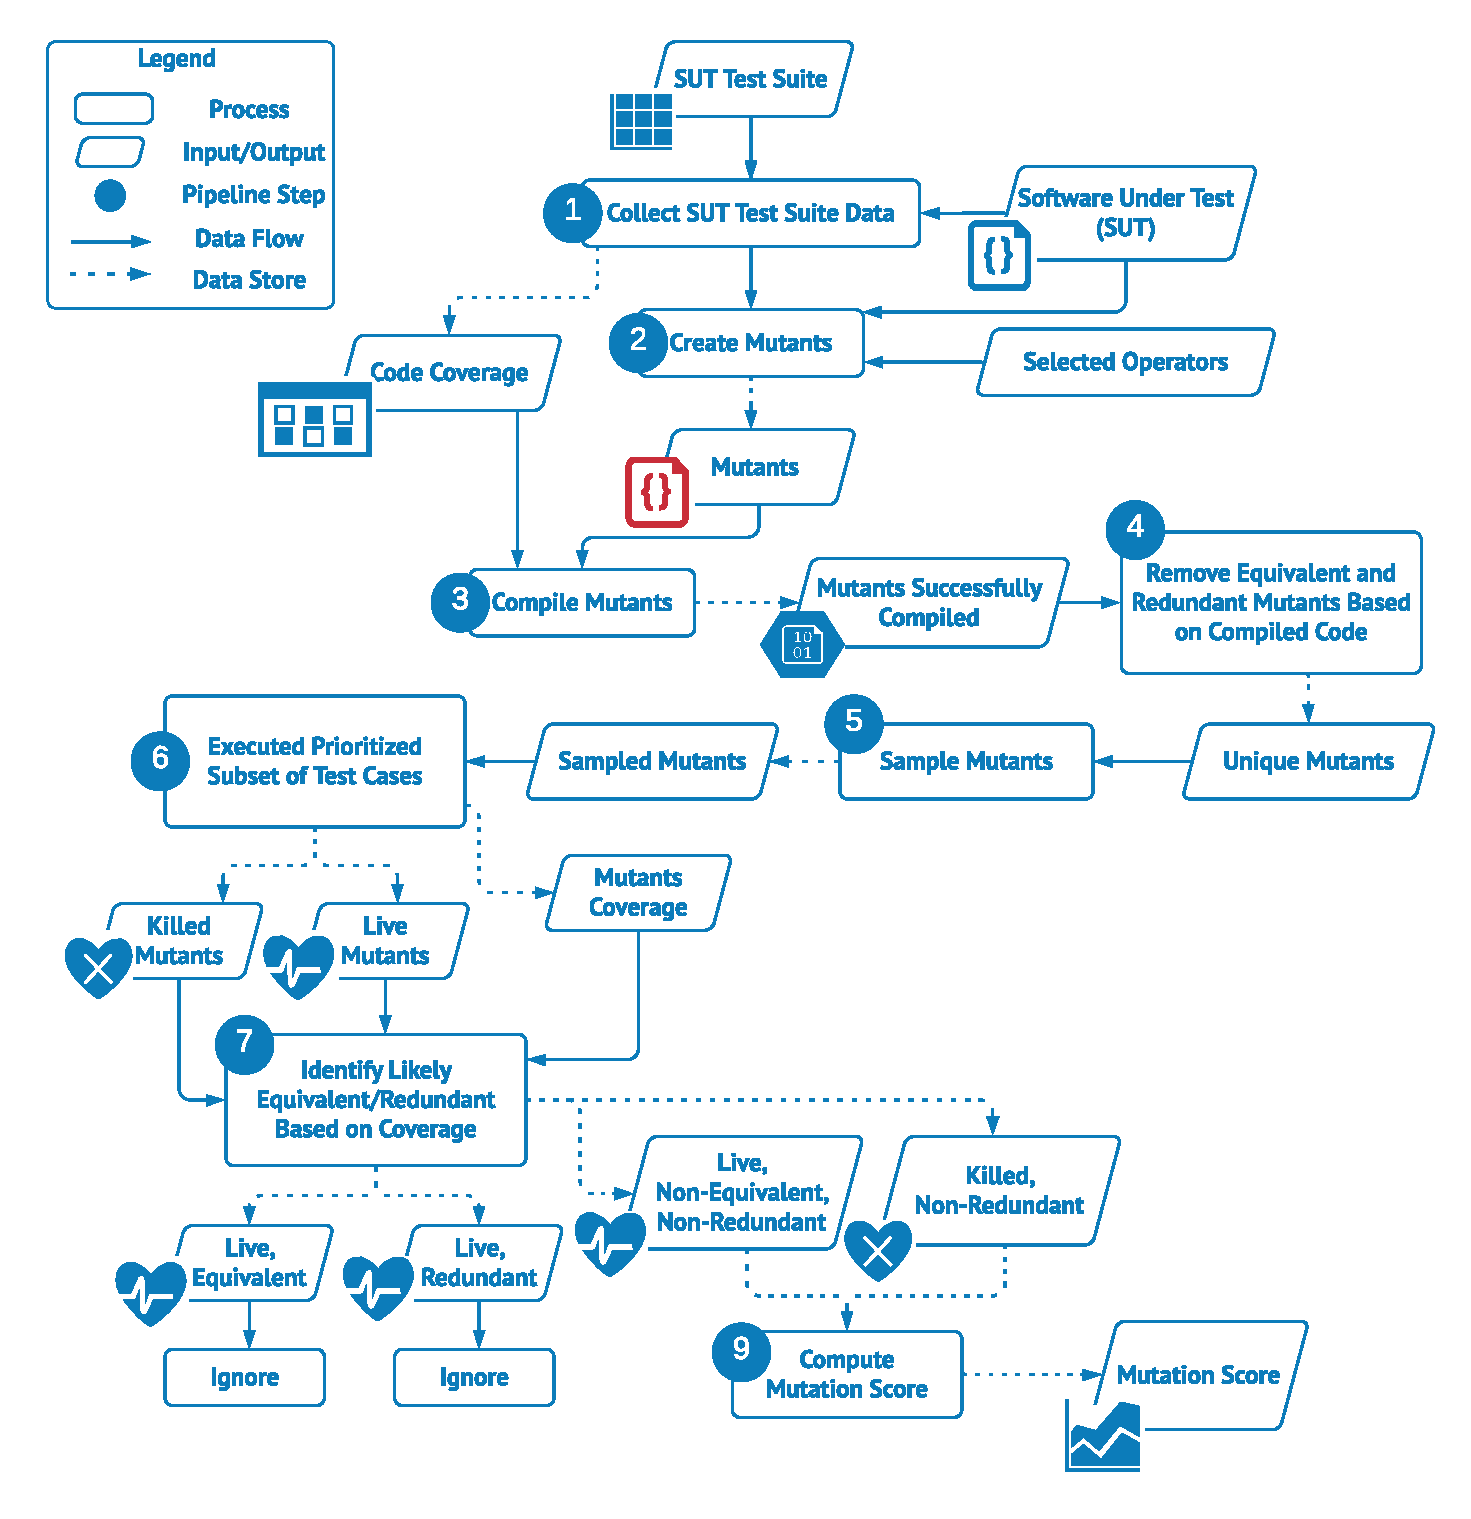
\includegraphics[width=\textwidth]{images/MT}
\caption{Overview of the proposed Mutation Testing Pipeline}
\label{fig:approach}
\end{center}
\end{figure}

Figure~\ref{fig:approach} provides an overview of the mutation testing process that we propose, namely Scalable Mutation Testing for Space Software  (\APPR). We describe each step in the following paragraphs. 

\subsubsection{Step 1}

In Step 1, the test suite is executed against the software under test (SUT) and code coverage information is collected. 
More precisely, we rely state-of-the art code coverage tools such as gcov~\cite{GCOV} and Vector CAST~\cite{VectorCAST} 
to record the number of times each line of code of the SUT has been exercised by a test case.

\subsubsection{Step 2}

In Step 2, we automatically generate mutants for the SUT by relying on a set of selected mutation operators.
In \APPR, based on the considerations provided in Section~\ref{sec:related:operators}, we rely on an extended sufficient set of mutation operators, which are listed in Table~\ref{table:sufficient_operators}.
In addition, in our experiments, we evaluate the feasibility of relying only on the SDL operators instead of the whole sufficient set of operators.

\input{tables/operators.tex}

To automatically generate mutants, we have extended SRCIRor~\cite{hariri2018srciror} to include all the mutation operators of the sufficient set. After mutating the original source file, our extension saves the mutated source file and keeps track of the mutation applied. 

\subsubsection{Step 3}
\label{codeDriven:stepThree}

In Step 3, we compile mutants by relying on the build system of the SUT. To this end, we have developed a toolset that, for each mutated source file: (1) backs-up the original source file, (2) renames the mutated source file as the original source file, (3) runs the build system (e.g., executes the command \texttt{make}), (4) copies the generated executable mutant in a dedicated folder, (5) restores the original source file. 

Build systems create one object file for each source file to be compiled and then link these object files together into the final executable. For this reason, since we modify at most two source files for each mutant (i.e., the mutated file and the file restored from previous mutation), we can reuse almost all the compiled object files in subsequent compilation runs, thus speeding up the compilation of multiple mutants. Some preliminary experiments conducted with our case study systems have shown that additional compile-time optimizations (e.g., mutant schemata) are not necessary to make the compilation of mutants feasible.

\MREVISION{C-P-24}{Mutants that lead to compilation errors are discarded. Concerning compilation warnings, we assume the build system of the SUT has been properly configured; more precisely, if the system should compile without warnings, the compiler is expected to be configured to treat warnings as errors otherwise mutants that lead to warning are retained.}

\subsubsection{Step 4}

In Step 4, we rely on trivial compiler optimizations to identify and remove equivalent and redundant mutants. 
\MREVISION{C-P-15}{We aim to enable all the available optimizations (e.g., \texttt{-O3} or \texttt{-Ofast} in GCC).}
If the SUT is already configured to be compiled with optimizations enabled, Step 4 consists of first computing the SHA-512 hash summary of all the mutant and original executables and then compare all the generated hash summaries. Hash comparison enables us to (1) determine the presence of equivalent mutants (i.e., mutants having the same hash of the original executable), and (2) identify duplicate mutants (i.e., mutants with the same hash). %Mutants that are identified as being either equivalent and redundant mutants are ignored in the following steps of \APPR. 
Equivalent and redundant mutants are discarded.
The outcome of Step 4 is a set of \emph{unique mutants}, i.e., mutants with compiled code that differs from the original software and any other mutant.

If the SUT should not be compiled with compiler optimizations enabled, we identify equivalent and redundant mutants by re-executing Step 3 with compiler optimizations enabled and then apply Step 4.
%The executables generated by this additional run of Step 3 are used only to identify equivalent mutants, not to evaluate the SUT test suite, which is based on executables compiled without optimizations (otherwise test cases may fail).

\subsubsection{Step 5}

In Step 5, we sample the mutants to be executed to compute the mutation score. This optimization is based on the results of Zhang et al.~\cite{zhang2013operator}, who compare eight strategies for sampling mutants. In our work, we consider two strategies. The first is the \emph{baseline sampling} strategy, which consists of randomly selecting $r\%$ mutants from the complete mutants set. The second is the \emph{method-based sampling} strategy, which is the best performing strategy in \cite{zhang2013operator} and consists of sampling mutants evenly across all functions of the SUT, i.e., sampling $r\%$ mutants from each set of mutants generated inside a same function.

%In Section~\ref{}, we evaluate which of these sampling strategies lead to mutation score


\subsubsection{Step 6}

In Step 6, we execute a prioritized subset of test cases. 
We execute test cases in sequence, and we select only the ones that satisfy 
the reachability condition (i.e., cover the mutated statement).
Similarly to the approach of Zhang et al. \cite{zhang2013faster}, we define the order of execution of test cases based on their likelihood of killing a mutant. However, we redefined the criteria for the selection of test cases because of the inapplicability of the ones proposed by Zhang et al. (see Section~\ref{sec:scalability}).


\MREVISION{C-P-46}{We execute only covered statements assuming that the test suite is optimal with respect to code coverage. More precisely, we addume that if a statement is not covered there is a good reason for it (e.g., it depends on hardware). 
If a statement is not covered by the test suite, there is no chance that a mutant generated in the non-covered statement can be possibly detected by any test case. 
If the test suite does not reach the required coverage there is no reason to perform mutation testing, because is already known that the test suite is not good.}
%\EMPH{When computing the mutation score, is it fare to not count those not-covered lines?}
%Yes, is it fare because mutation testing assess the quality of existing test suites, and considering non-covered statements would be out of the scope of the technique. Also, including non-covered statements into the mutation score, would not let us to assess correctly the quality of the existing test suite.
%\EMPH{Maybe the approach would be to run the test augmentation process to provide test cases for the missing statements?}
%Yes, the same tools used for test augmentation can be used. We can run them. The main difference is that oracles  for the generated test cases should be manually specified (in the case of test augmentation we may derive the oracle based on the values generated by KLEE/CBMC). However, the evaluation of these generated test suites through mutation testing address a different research question than the one of the project; i.e., we would evaluate test automation tools instead of manual test suites.




%However, we notice that such optimization may not be sufficient when test suites are particularly large; indeed, prioritizing test cases may not be sufficient to reduce execution time. For example, live mutants may lead to the execution of a large number of test cases when almost all the test cases of the test suite exercise the mutated statement. 


To reduce the number of test cases to be executed with a mutant, 
we should first execute the ones that more likely satisfy the necessity condition. 
More precisely, the next test case to be executed in a sequence should be the one that exercises the mutated statement with variable values not observed before. 
Unfortunately, in our context, the size of the SUT and its real-time constraints prevent us from recording all the variable values processed during testing. 

To determine if two test case executions exercise the mutated statement with diverse variable values, we rely on code coverage.
% as a surrogate indicator of  variable values diversity.
%diversity in values assigned to the variables used in a statement. 
Indeed, a difference in the set of instructions being covered by two test cases that exercise the mutated statement may depend on the values used in the mutated statement. 
However, since the behaviour of the whole software depends on all the executed software instructions, we reduce the scope of our code coverage analysis 
%to the file containing the source code of the mutated function. 
to the mutated function, its callers, and its callees.
%to maximize the chances that a change in the behaviour of the software depends on the values used in a mutated statement, we determine that two executions likely exercise a mutated statement with diverse values by focussing on the coverage of 
%the mutated function, its callers, and its callees.
A reduced scope is effective in determining behavioural differences based on the analysis of variable valuations~\cite{Pastore:VART:2014}.

%Since related work focuses on either statement coverage or the frequency of execution of a statement, 
Following related work, we have identified two possible criteria to characterize test case executions based on code coverage:
\begin{itemize}
\item[C1] Identify the set $C_t$ of source code statements being covered by the test case.
%\item[C2] Identify the set of unique pairs $\langle\mathit{statement},\mathit{arity}\rangle$, where $\mathit{statement}$ is a unique identifier for the source code statement, and $\mathit{arity}$ is a symbol (i.e., $1$ or $*$) indicating if the statement has been covered one or more times.
\item[C2] Derive a vector whose values capture the number of times each monitored statement had been covered.
\end{itemize}

We have identified distance metrics that determine how dissimilar two test cases are, and, consequently how likely they exercise the mutated statement with different values. In the case of C1 we rely on the Jaccard and Ochiai index, which are two similarity indexes for binary data successfully used to compare program executions based on code coverage~\cite{Zou:Ochiai:2019,Keller:Jaccard:2017,Briand:2019}. Given two test cases $T_A$ and $T_B$, the Jaccard  ($D_J$) and the Ochiai ($D_O$) distance are computed as follows:

$D_J(T_a,T_b)=\frac{|C_a \cap C_b|}{|C_a \cup C_b|}$ \hspace{5mm} $D_O(T_a,T_b)=1-\frac{|C_a \cap C_b|}{\sqrt{|C_a| * |C_b|}}$, 
$C_a$ and $C_b$ are the set of coverage items exercised by the test cases $T_a$ and $T_b$, respectively.

In the case of C2, we compute the distance between two test cases by relying on the euclidean distance ($D_E$) and the cosine similarity distance ($D_C$), two popular distance metrics used in machine learning. Given two vectors $V_A$ and $V_B$ that capture the number of times each statement has been covered by test cases $T_A$ and $T_B$, the distances $D_E$ and $D_C$ can be computed as follows:

$D_E=\sqrt{\sum_{i=1}^{n}(A_i-B_i)^2}$ 
$D_C= \frac{\sum_{i=1}^{n}A_i*B_i}{\sqrt{\sum_{i=1}^{n}{A_i}^2}*\sqrt{\sum_{i=1}^{n}{B_i}^2}}$,
%Their main difference is that cosine similarity is used when the magnitude of the vectors should not matter.
$A_i$ and $B_i$ refer to the number of times the i-th statement had been covered by test cases $T_A$ and $T_B$, respectively.

Figure~\ref{alg:prioritize} shows the pseudocode of our algorithm for selecting and prioritizing test cases. It generates as output
a prioritized test suite (i.e., \emph{PTS}) that consists of a subset of the test cases that exercise the mutated statement (Line~\ref{alg:prioritize:select}).
Based on the findings of Zhang et al. \cite{zhang2013faster}, we first select the test case that exercises the mutated statement more times (Line~\ref{alg:prioritize:first}) \MREVISION{C-P-17}{ and add it to the prioritized test suite (Line~\ref{alg:prioritize:add}).}
Then, the next selected test case is the one with the largest distance from the closest test case belonging to the set of test cases already selected (Lines~\ref{alg:prioritize:selectStart} to~\ref{alg:prioritize:selectEnd}). 
%is most different than any other test case already included in the prioritized test suite.

%Then, since we aim to maximize test cases diversity, the next selected test case should be the one that is most different than any other test case already included in the prioritized test suite.
%For this reason, for each test case $n$ not selected yet (Line~\ref{alg:prioritize:notSel}), we identify the test case $t$ showing the most similar coverage (i.e., the one with the minimal distance $d$, Line~\ref{alg:prioritize:minD}). We then select the test case $n$ with the highest distance from its closest test case (Lines~\ref{alg:prioritize:selectStart} to~\ref{alg:prioritize:selectEnd}). 

The algorithm iterates as long as it identifies a test case that exercises 
the program instructions differently than the test cases already selected (Line~\ref{alg:prioritize:until}).

Test cases are then executed in the selected order. During the execution we collect code coverage information and identify killed and live mutants.

\input{algos/selection.tex}

\subsubsection{Step 7}


In Step 7, we identify likely equivalent and likely redundant mutants by relying on code coverage information.

Differently from related work~\cite{schuler2013covering}, since the size of a program may impact on the number of statement that present coverage differences because of non-determinism, 
to identify equivalent and redundant mutants through a threshold, instead of relying on the absolute number of methods/statements presenting differences in code coverage, we compute normalized distances based on the distance metrics $D_J$, $D_O$, $D_E$, and $D_C$. 

%To identify equivalent mutants, we select the
A mutant is considered non-equivalent when the distance from the original program is above the threshold $T_E$, for at least one test case.
Similarly, a mutant is considered non-redundant when the distance from every other mutants is above the threshold $T_R$, for at least one test case.

\MREVISION{C-P-19}{Figure~\ref{alg:nonEquivalent:nonRedeundat} shows the algorithm for detecting non-equivalent and non-redundant mutants.
It first identify among the list of killed mutants all the non-redundant ones (Line~\ref{alg:equivalent:KNR}).
Then it identifies the non-equivalent mutants among the list of live mutants (Line~\ref{alg:equivalent:LNE}).
Finally, it further filters the list of non-equivalent mutants to keep only the ones that appear to be non-redundant (Line~\ref{alg:equivalent:LNENR}).}

\input{algos/equivalentRedundant.tex}

\subsubsection{Step 8}

The mutation score is computed as the ratio between the number of live, non-equivalent and non-redundant mutants  and the overall number of non-equivalent, non-redundant mutants identified in Step 7:

$\mathit{mutation}\ \mathit{score} = \frac{|\mathit{LNENR}|}{|\mathit{LNENR}|+|\mathit{KNR}|}$,
$\mathit{LNE}$ is the number of live, non-equivalent, non-redundant mutants,
$\mathit{KNR}$ is the number of killed non-redundant mutants.

%Similarly,
%
%obof at lest one test case with respect
%
%
%The code coverage difference between the mutant and the original program is represented by a \textit{threshold T\%}, a difference of code coverage over a certain T\% indicates that both versions are not equivalent.


% !TEX root =  ../MAIN.tex
\subsection{Overview}

We address the following research questions:

%    \item RQ1 Is data-driven mutation cost affordable within the space context? This research question aims to determine if data-driven mutation testing is feasible in terms of costs related to the set-up of the system.
%    What to measure? Size of fault models. Lines of code added to inject probes.
%    
%    %% oscar notes:
%    % - the first question is, we need a definition of feasible in terms of cost related to the setup of the system
%    %   - what is the baseline? 
%    %   - how do we measure the cost of setting up data-driven (implementation complexity)?
%    %.    - human cost of setting up the fault model?
%    %     - size of the SUT in memory?
%    %     - SUT execution time per introduced fault, which is the fastest? \cite{winter2011impact}
%    %.      - given that a system may behave differently depending on the effect of the fault, the faults could be classified as no effect, test failure, application hang
%    %     - LoC (SLoCCount)
%    %     - cyclomatic complexity (SourceMonitor)?
%    % - injecting defects in every location of complex software leads to a dramatic increase of the cost of the campaign \cite{natella2012fault}
%    
%    %  - fault latency: addresses the duration of an injection in terms of repeated fault activation. Transient faults are activated exactly once, intermittent faults are activated a finite number of times, and permanent faults are activated every time.
%    % - injection trigger: when the probe is activated \cite{winter2011impact}
%
%    \item RQ2 Does data-driven mutation scale in space context? Given the large quantity of data exchanged by space software components, there is a risk that data-driven mutation require the execution of a large number of test cases. This research question aims to determine if data-driven mutation testing can scale up.
%
%    \item RQ3 How does data-driven mutation compare to code-driven mutation in terms of effectiveness and test execution time? This research question aims to compare the results obtained with code-driven and data-driven test suite assessment. We are interested in answering the following subquestions: 
%    \begin{itemize}
%    \item (RQ3.a) Do test cases that kill code-driven mutants tend kill also data-driven mutants? 
%    
%    %For each data-driven mutant we remove all the test cases (or, better, the oracles) that kill the mutant, then we verify if the code-driven mutation score changes. If the code-driven mutation score does not change it means that data-driven is complementary.
%    
%    %For each code-driven mutant we remove all the test cases that kill the mutant, then we verify if the data-driven mutation score changes
%    
%    %We shall consider only  code-driven mutants affecting the functionalities affected  by data-driven mutation.
%    
%    \item (RQ3.b) What type of mutants generated by data-driven mutation are not detected by means of code-driven mutants? 
%    
%    %We keep a minimal set of test cases to kill all the data driven mutants
%    %We look for test cases that if removed do not change the code-driven mutation score
%    %If such test cases exists, it means that the data driven mutant that they kill, cannot be replaced through a code-driven mutant
%    
%    \item  (RQ3.c) Is it possible to find a relation between the mutation scored computed with data-driven and code-driven mutation?
%    Measurements. Simple solution: (1) collect mutation score for code-driven and data-driven for all the subjects (2)  compute some correlation coefficient. Problem: too few subjects, not sure if correlation coefficient works with 3 subjects only. What does literature says on this matter?
%    
%    \item (RQ3.d) Is data-driven mutation better than code-driven mutation in detecting test suites not capable of identifying problems in the implementation of requirements?
%    
%    We assume that data-driven simulates fault in the implementation of requirements. Is it really the case?
%    Does it improve over code-driven?
%    
%    To this end we inject faults in the software (e.g., faults manually derived after modifying the requirements) and compare how well data-driven/code-driven discover them.
%    
%    We identify test suites with mutation score of 70\%, 60\%, 50\%
%    or we identify test suites achieving >90\% of the subject mutation score, >80\%, >70\%.. 
%    With "identify" I mean we select a subset of test cases  in the original test suite, to achieve the desired mutation score.
%    We compute the percentage of faults detected by the test cases killing at least one data-driven mutant.
%    We compute the percentage of faults detected by the test cases killing at least one code-driven mutant.
%    \end{itemize}
%    
%
%    \item RQ4 To what extent equivalent and redundant mutants affect data-driven mutation? We aim to investigate how likely data-driven mutants are affected by the presence of equivalent and redundant mutants.
%
%    \item RQ5 Does mutants sampling lead to accurate results in the case of data-driven mutation testing? This re- search question investigates if mutants sampling is accurate also in the case of data-driven mutation testing.
%
%
%    \item RQ6 How do mutants sampling approaches compare in terms of performance? We aim to determine which mutants sampling strategy reduces most the data-driven mutation testing execution time.
%


\emph{RQ1. What are the types of test suite shortcomings identified by \APPR?}
    We aim to assess the effectiveness of \APPR in identifying various test suite shortcomings.  In other words, we want to know if mutation analysis based on \APPR can provide clear guidance in terms of what to improve in a test suite. 
   % Further, we will discuss with engineers the reasons why mutants are not killed by the test suite and categorize  such shortcomings, e.g., lack of oracles verifying warning messages.
    %This research question aims to determine the test suite weaknesses by identifying the shortcomings of the test suites (e.g., lack of oracles).
    % This research questions aims to identify the type of faults that are harder to kill among CPSs test suites.

%FABRIZIO: the following has been removed for space reasons...
%\emph{RQ2. How are killed and live mutants distributed among mutation operators?}
%We study the distribution of killed mutants across mutation operators to determine if it is feasible to identify a subset of operators that is more effective than others in detecting test suite shortcomings.
  



    
\emph{RQ2. 
What is the impact of equivalent and redundant data-driven mutants on the mutation analysis process?}
    In general, mutation analysis may lead to the generation of equivalent and redundant mutants.  
    In the specific context of \APPR, we analyze the extent of their impact on mutation scores.
    %by re-calculating the mutation execution time and mutation score when removing such mutants from the analysis.}

\emph{RQ3.  Is data-driven mutation feasible?}
    To assess its feasibility in practice, we evaluate the cost of setting up data-driven mutation analysis (i.e., defining fault models and instrumenting the CPS with probes), {the duration of the mutation analysis process, and the} runtime overhead introduced during test case execution.    

\subsection{Subjects of the study}

%\input{DDMA/tables/subjects}

%To assess our research questions, we considered five software artifacts, developed by two of our industry partners for different satellites:  Attitude Determination And Control System (\ADCS), \GPS, Payload Data Handling Unit (\PDHU), the three subsystems developed by \LuxSpace for the \ESAIL satellite, and the Parameter system (\PARAM), CSP networking (\CSP) libraries developed by \GomSpace.

To assess our research questions, we consider \PARAM, which is a client-server component to manage configuration parameters in cubesats.
Also, we examine three \ESAIL software sub-systems (1) the Attitude Determination And Control System (\ADCS), the Global Positioning System (\GPS), and the Payload Data Handling Unit (\PDHU). {These are representative examples of control and utility software, as well as sensor and actuator drivers.} Detailed information about the fault models is provided in Appendix~\ref{appendix:FMS}.

We rely on \APPR to evaluate the \PARAM integration test suite by  mutating the data exchanged between the client and server components of \PARAM.
Similarly, \APPR is used to evaluate how well the 
\ESAIL test suite covers interoperability problems affecting the integration between the control software of \ESAIL (hereafter, CSW) and the \ADCS, \PDHU, and \GPS components. We thus
mutate the data exchanged between \ESAIL CSW and these three components.
Since each of these sub-systems have a  different purpose (i.e., their data is processed by distinct CSW functions and affect distinct \ESAIL features) we treat them as distinct case study subjects although they are tested using the same test suite. We focus on the \ESAIL test suite that makes use of an SVF to simulate the \ADCS, \PDHU, and \GPS components. 
The main reason is that these three components can only be executed on the target hardware and thus most of the scenarios involving them are tested in a simulated environment first.
\CHANGED{We do not mutate messages or data items that are tested only with HIL.}

In the case of \PARAM, we inject mutation probes into the \PARAM server to mutate both received and generated messages. For \ESAIL, we insert mutation probes into the SVF that mutate the messages it generates; we avoid mutating the messages received by the SVF because such mutations may lead to input data it does not support. 
%Table~\ref{table:summary} provides further information about our case study subjects.
\ESAIL features 74 kLoC and its SVF 65 kLoC. 
The \ESAIL test suite includes 384 test cases, takes approximately 10 hours to execute, and relies on three simulated
\SVF sub-systems (i.e., \ADCS, \GPS, and \PDHU).
Instead, \PARAM contains 3 kLoC and is tested through an integration test suite which is composed by 170 test cases. 
The \PARAM integration test suite takes approximately 1 minute to execute.
By considering both a quick integration test suite and an extensive system test suite, we aim to cover the diversity of scenarios in which our approach can be applied.


%\GomSpace subject is compiled with the Gnu Compiler Collection (GCC) for Linux x86 version 6.3.
%Instead, \LuxSpace subjects rely on Clang++ Compiler for Linux x86\_64 version 5.0.0.


\subsection{Experimental Setup}


With the support of our industry partners, we relied on  
 the systems' specification documents 
 %(i.e., the Interface Control Document and the Software User Manual, based on the ECSS standard) 
 to define the fault models for each subject.
 

%Note that we did not target every data item being exchanged between components, since input partitions for certain data items (e.g., nominal and non-nominal cases) are covered only by test suites with hardware in-the-loop.

% we based on the specifications of the systems, provided the type of ECSS document, and selected only operators that cover a fault that shall be discovered by the test suite 

% (i.e., the rest of faults are covered by test suites with hardware in-the-loop). 
%We used this information as an input for \APPR and consequently applied the six steps of the approach.

\input{DDMA/tables/operators_summary.tex}


{Table~\ref{table:summary} provides information about the fault models.}
The fault models (FMs) for the \ADCS include multiple configurations (\emph{Configured operators}) of eight mutation operators: BF, VAT, VBT, VOR, IV, FVOR, FVBT, and FVAT.
The \PDHU fault models include four operators: BF, IV, VAT and FVAT.
Even though the \GPS fault model concerns only one data type, it makes use of six operators: ASA, HV, IV, SS, VAT, and FVAT.
For \PARAM, we relied on the operators BF, HV, IV, SS, VAT, and FVAT.
All the mutation operators provided by \APPR have been used in at least one fault model, which shows their usefulness.
{They have led to 172 mutation operations for \ADCS, 23 for \GPS, 29 for \PDHU, and 80 for \PARAM; the number of configured operators and mutation operations match except when we rely on VOR and FVOR.}

%Table~\ref{table:summary} provides information about the different fault models that were specified, which consist of 119 mutation operations for \ADCS, 26 for \GPS, 59 for \PDHU, and 35 for  \PARAM.
%, and \TODO{ZZ} for the \CSP.
%After considering all the mutation operators specified in Table~\ref{table:operators}, for \ADCS, this led to five mutation operators: BF, VAT, VBT, VOR, and IV. 
%Similarly, in the case of \PDHU, 
%we considered four mutation operators: BF, IV, VAT and FVAT.
%Even though the \GPS fault model concerns only one data type, it makes use of five mutation operators: ASA, HV, IV, SS, and VAT.
%For \PARAM, we made use of the mutation operators BF, HV, IV, SS, and VAT. 
%Since all the mutation operators have been used in at least one fault model, we can consider all of them to be useful.

%In general, our subjects include \TODO{the same} ratio of operators per fault model specification,%type,
 %thus showing that all operators are useful.

We performed our experiments using an HPC cluster with Intel Xeon E5-2680 v4 (2.4 GHz) nodes.

%To perform our empirical evaluation, 
%We implemented \APPR in a toolset that is available under the ESA Software Community Licence Permissive, at the following URL \textbf{https://blind/}.


\subsection{RQ1 - Approach effectiveness}

% \subsubsection*{Design and measurements}

We analyzed the extent to which \APPR helps identify limitations in test suites.
For each subject, we inspected uncovered fault models, uncovered mutation operations, and live mutants. We then analyzed how they could potentially be explained by the types of possible shortcomings:
untested message types (UMT), uncovered input partitions (UIP), poor oracle quality (POQ), and lack of test inputs (LTI).
To achieve the above, we proceeded as follows.
For each uncovered fault model, we discussed with developers if the functionality triggering the exchange of the targeted message was tested by the test suite.
For uncovered mutation operations, we discussed with engineers if they match an uncovered input partition.
For live mutants, we determined if they could be killed by improving test oracles (see how equivalent mutants are detected for RQ2).
%(e.g., lack of oracles concerning internal state variables, lack of inputs triggering exceptional scenarios).

To address RQ1, based on the above analysis, we discuss below how our metrics (i.e., \emph{fault model coverage - FMC}, \emph{mutation operation coverage - MOC}, and \emph{mutation score - MS}) relate to the predefined shortcoming categories {(e.g., a low mutation score may indicate missing test oracles)}.
%For example, a low mutation score may indicate missing test oracles, or a low fault model coverage level may suggest a lack of test cases for certain functionalities.
\CHANGED{Further, to understand how variations in test effectiveness could be explained, we investigate how our metrics relate to the number of functionalities under test (i.e., the number of fault models - $\mathit{FM}$), the number of mutation operations ($MO$), and the number of covered mutation operations ($CMO$), respectively. 
To get an idea of observable trends, we compute the Spearman's correlation coefficients between them, hereafter denoted $\rho_{FM}$, $\rho_{MO}$, $\rho_{CMO}$.}

%Concerning UIP and POQ we distinguish between nominal and non-nominal scenarios. 
%\emph{UIP for non-nominal (nominal) scenarios} indicate that the test suite triggers the exchange of data items targeted in the fault model but it does not exercise the non-nominal (nominal) cases. For example, the test suite may cause the retrieval of the board voltage only in the case of voltage within range.
%\emph{POQ for non-nominal (nominal) scenarios} indicate that the test suite triggers the exchange of data item instances that are representative for the non-nominal (nominal) case (e.g., error messages are exchanged by components) however the oracles do not appropriately verify outputs. For example, the test suite may not verify if error messages had been actually exchanged.



%Furthermore, for each subject, we report the mutation analysis results in terms of the metrics defined in Section~\ref{sec:mutantsExecution}: \emph{fault model coverage}, \emph{mutation operation coverage}, and \emph{mutation score}.



%A description of the possible shortcomings that can be identified by \APPR follows.
%The possible shortcomings that can be identified by \APPR had been introduced in Section~\ref{}:
%untested message types (UMT), uncovered input partitions (UIP), poor oracle quality (POQ), and lack of test inputs (LTI).
%To better characterize our results we have refined UMT, UIP, and POQ into subclasses that are reported in the following.
%
%\emph{UMT - Functionality not tested:} the test suite does not exercise the exchange of the messages targeted by the given fault model because engineers mistakenly forget to test one functionality. 
%%This type of shortcoming can be reflected on the \emph{fault model coverage} metric.
%
%%\emph{Lack of input partitions for a functionality} means the test suite includes a testing scenario, but it does not include configurations for a component related to the targeted data item.
%
%\emph{UIP - Lack of simulations for nominal scenarios:} the test suite triggers the exchange of the targeted data items but it does not exercise the nominal case (e.g., it tests the retrieval of the board voltage only in the case of voltage out of range).
%\emph{UNIP - Lack of simulations for non-nominal scenarios:} the test suite triggers the exchange of the targeted data items but it does not exercise the nominal case (e.g., it tests the retrieval of the board voltage only in the case of voltage within range).
% 
%%Lack of simulated configurations and input partitions are reflected on the \emph{mutation operation coverage} metric.
%
%\emph{Lack of oracles concerning log-files from hardware} means that the test suite covers a testing scenario for the targeted data item, and includes test cases for a specific input partition, but it does not verify possible warnings coming from hardware components.
%\emph{Lack of oracles for return codes} means that the test suite covers the testing scenario and input partition, but it does not verify the return codes coming from a certain component.
%\emph{Lack of oracles concerning non-nominal scenarios} means that the test suite covers the exceptional testing scenarios and input partitions, but it does not verify if warnings are produced, but simply check that redundancy mechanisms work.
%\emph{Lack of oracles concerning internal state variables} means the test suite covers a testing scenario and a specific input partition, but it does not verify internal or intermediate state variables.
%Lack of oracles reflects directly on the \emph{mutation score} metric.


\subsubsection*{Results}

\input{DDMA/tables/results_ms}

\input{DDMA/tables/shortcomings}

Table~\ref{table:mutationresults} reports the mutation analysis results according to our metrics (see D2).
In Table~\ref{table:shortcomings}, we report how uncovered fault models, uncovered mutation operations, and live mutants are distributed with respect to the different shortcomings we noticed on each subject.

Concerning \emph{fault model coverage}, \ADCS reached a coverage of 90.00\%, while \GPS, \PDHU, and \PARAM all achieved 100\%.  
%$\rho_{FM}$ = -0.90, 
%$\rho_{FM}$ = -0.77, 
%we see that, 
As expected, the much higher number of messages to test for \ADCS leads to incomplete testing. 

\ADCS reached 74\% \emph{mutation operation coverage}. \GPS, \PDHU, and \PARAM  achieved even higher coverage with 95.65\%, 82.76\%, and 91.25\%,  respectively. Since 
%$\rho_{FM}$ = -0.97 and $\rho_{MO}$ = -0.98, 
%$\rho_{FM}$ = -1 and 
$\rho_{MO}$ = -0.8, results suggest that lower mutation operation coverage is more likely when systems are more complex (i.e., there are many mutation operations, whose numbers depend on the number of input partitions). 

Regarding \emph{mutation scores}, we report 45.00\% for \ADCS,  95.45\% for \GPS,  and 100.00\% for \PDHU. These results indicate a varying performance of the \SVF test suite across sub-systems.
\PARAM obtained a mutation score of 38.36\%, indicating that only slightly more than a third of mutants are killed by the test suite.
Given that 
%$\rho_{FM}$ = -0.80, $\rho_{MO}$ = -0.80, and $\rho_{CMO}$ = -0.86, 
%$\rho_{FM}$ = -0.6, $\rho_{MO}$ = -0.6, and 
$\rho_{CMO}$ = -0.6, 
we conclude that the mutation score tends to be lower for complex systems with a large number of covered mutation operations.
%Different from the other metrics,  mutation scores do not appear dependent on the size of the fault model.

Table~\ref{table:shortcomings} provides the shortcomings identified for all our subjects. 
Our analysis confirms that (1) uncovered fault models (i.e., low \emph{FMC}) indicate lack of coverage for certain message types (\emph{UMT}) and, in turn, the lack of coverage of a specific functionality (i.e., setting the pulse-width modulation in \ADCS); (2) uncovered mutation operations (i.e., low \emph{MOC}) highlight the lack of testing of input partitions (\emph{UIP}); (3) live mutants (i.e., low \emph{MS}) suggest poor oracle quality (\emph{POQ}). In our case study systems the presence of live mutants was not explained by the lack of test inputs in the original test suite. Moreover, we have not uncovered latent faults, which is unsurprising given that all these systems went through all testing stages, including HIL, and are on orbit. 

%\subsection{RQ2 - Operators effectiveness}
%
%% \subsubsection*{Design and measurements}
%%RQ2 aims to investigate differences in results across \APPR operators. 
%A mutation operator is effective if it leads to mutants that enable detecting uncovered input partitions, poor oracle quality, or lack of test inputs. For each subject, we thus report the proportion of mutation operators that lead to such cases (i.e., mutants that are hard to kill).
%In general, hard to kill mutants indicate to practitioners how to prioritize the execution of mutants during the data-driven mutation analysis process (hard to kill mutants shall be executed first).
%
%
%
%We identify the type of faults that are harder to kill by analyzing the mutation scores across operators.%distribution of killed mutants across operators.
%In general, faults that are harder to kill may indicate to practitioners which fault types to prioritize during the data-driven mutation analysis process.%, since they may hide subtle problems of the test suite.
%
%%We measure the proportion of shortcomings detected by prioritizing the execution of operators.
%
%% For each subject, we report the coverage metrics defined in  Section~\ref{sec:mutantsExecution}: \emph{fault model coverage},  \emph{mutation operation coverage}, and \emph{mutation score}.
%
%\subsubsection*{Results}
%
%%Operators that are killed most are the ones that concern data provided by sensors, which is often the one verified by test cases.
%%The operator that is less killed is the BF, which is used for configuration options or state information that is usually not verified by the oracles.
%%
%%
%%
%%\TODO{TBD}
%
%\input{DDMA/tables/killed_fault_classes}
%
%Table~\ref{table:killed_fault_classes} presents the distribution of hard to kill mutants across the types of mutation operators implemented by \APPR. In general, it is not feasible to identify a subset of operators that is more effective than others; indeed all the operators show a varying proportion of hard to kill mutants across subjects. Such result may be due to our set of operators being representative and reduced. 
%



\subsection{RQ2 - Equivalent and redundant mutants}

% \subsubsection*{Design and measurements}

As they potentially have significant impact on the applicability of any mutation analysis approach, we assess the impact of equivalent and redundant mutants generated by \APPR.  
%Equivalent and redundant mutants inflate the mutation score and thus prevent the correct assessment of the test suite. This question aims to determine whether this is a significant problem with \APPR.

%Equivalent mutants are modified versions of the SUT that have the same visible output as the original SUT. 
%Instead, redundant mutants are modified versions of the SUT that have the same visible output as other mutants (e.g., two mutants causing the same failures in the test suite).

% consist of modified data (i.e., data altered by means of mutation operators) that do not lead to any noticeable difference in the output of the SUT with respect to the original version of the data.
%Instead, redundant mutants cause the same failures in the test suite.%, and consequently inflating the mutation score.%preventing the correct assessment of the test suite. 
%Two are the reasons for redundant mutants. First, 
%The reason for redundant mutants is that 
%mutations alter different instances of a same data structure in the same way (e.g., delete a message in a sequence). 

%Second, the mutations alter data chunks that are ignored by the oracles of the test suite. 

%For every subject, we report the number of equivalent and redundant mutants. 
We determined if a live mutant is nonequivalent by verifying, with the support of our industry partners, 
if there existed a test case that, after performing the mutation operation, would generate one observable output (e.g., log entry, state variable, or data sent in response to test inputs) that differs from the one generated by the original program. Otherwise a mutant was considered equivalent.

According to related work, two mutants should be considered redundant if they produce the same observable output for every possible input~\cite{Shin:TSE:DCriterion:2018}.
%Recent research work has shown that two mutants shall be considered redundant only if it is not possible to identify inputs that distinguish them~\cite{Shin:TSE:DCriterion:2018}; in turn, two mutants are redundant when they produce the same observable output for every possible input. 
Since, with large software systems, it is not possible to automatically determine if such condition holds (e.g., differential symbolic execution may not scale and is hardly applicable when components communicate through a network), we rely on manual inspection. To make such such analysis feasible, we first need to select a subset of mutant pairs that are likely to be redundant (e.g., mutants that produce the same output for every executed test case). 
However, the size of the software systems under analysis prevents the collection of all the observable outputs produced by the system. 
%(e.g., only the filtering of nondeterministic data such as timestamps requires a great deal of effort and domain knowledge); for this reason we focus on the data processed by assertions. 
%Unfortunately, it is not feasible to simply collect the data processed by assertions because assertions often process aggregated results generated by test utility functions (e.g., to determine if loss of  communication between \ESAIL-CSW and \ADCS has been detected, reported, and recovered it is necessary to inspect log files for the presence of corresponding log entries in appropriate order). 
We thus select as likely to be redundant all the pairs of killed mutants that (1) are exercised by the same test cases and (2) present the same failing assertions for every test case. We then manually inspect the test cases to determine if an additional assertion or a different test input might lead to different results for the two mutants. Similar to related work, we exclude live mutants from this analysis~\cite{papadakis2016threats}.

%Since, with large CPSs, it is not possible to automatically determine if such condition holds (e.g., differential symbolic execution is not applicable when components rely on floating point arithmetic or communicate through means different than method calls), we shall rely on manual inspection. To make such analysis feasible, we first need to select a subset of mutant pairs that are likely redundant, that is, mutant pairs that produce the same output for every executed test case. 
%However, the size of the CPSs under analysis prevents the collection of all the observable outputs produced by the system (e.g., only the filtering of nondeterministic data such as timestamps requires a great deal of effort and domain knowledge); for this reason we focus on the data processed by assertions. Unfortunately, collecting the data processed by assertions is not straightforward because assertions often process aggregated results generated by test utility functions, e.g., to determine if loss of  communication between \ESAIL-CSW and \ADCS has been detected, reported, and recovered it is necessary to inspect log files for the presence of corresponding log entries in appropriate order. 
%We thus select as likely redundant all the pairs of killed mutants that (1) are exercised by the same test cases and (2) present the same failing assertions for every test case. We then manually inspect the test cases to determine if an additional assertion or a different test input (e.g., different simulator configuration) may distinguish the two mutants. Similarly to related work, we exclude live mutants~\cite{papadakis2016threats}.




%\input{DDMA/tables/eq_red}

%\input{DDMA/tables/oraclesShortcomings}

%Table~\ref{table:eq_red} provides the results. 

\subsubsection*{Results.} 
All live mutants (i.e., 55 mutants for \ADCS, 1 mutant for \GPS, and 45 mutants for \PARAM) generate outputs that differ from the original software system and, therefore, we did not detect any equivalent mutant. Though it needed to be confirmed, such result was expected since our methodology, if correctly applied, suggests, for every data item, a set of mutation operators that, by construction, should not lead to mutated data that is equivalent to the original data.
Live mutants can be killed by introducing oracles that (1) verify additional entries in the log files (39 instances for \ADCS, 1 instance for \GPS), (2) verify additional observable state variables (14 instances for \ADCS, 45 instances for \PARAM), and (3) verify not only the presence of error messages but also their content (2 instances for \ADCS).


We did not find redundant mutants either, which was expected since (1) mutations concerning different data items, by definition, are expected to lead to different outputs, (2) the set of operators applied to a same data item, if selected according to our methodology, cannot lead to mutated data that is redundant.
All the pairs of likely redundant mutants were due to five situations: (1) the test case does not distinguish failures across data items (e.g., temperature values collected by different sensors), 
(2) the test case does not distinguish errors across different messages (e.g., in \ADCS, the IfHK message reporting a broken sensor or the message sent by a sensor reporting malfunction), (3) the test case does not distinguish between errors in nominal and non-nominal data (e.g., it does not distinguish between VOR and FVOR), (4) the test case does not distinguish between upper and lower bounds (e.g., the mutants for VOR lead to the same assertion failures), and {(5) the test case does not distinguish between different error codes (i.e, it simply verifies that an error code is generated)}. Addressing such shortcomings make test cases more useful for root cause analysis.

\subsection{RQ3 - Feasibility}

% \subsubsection*{Design and measurements}
The feasibility of data-driven mutation analysis depends on the required manual effort, which includes defining fault model specifications and injecting probes into the SUT source code. Also, the overhead introduced at runtime by the execution of the mutation operations may introduce delays in real-time systems and consequently cause failures. Finally, feasibility also depends on the overall duration of the mutation analysis process. 

To discuss manual effort, we measured, for each subject, (1) the number of {rows in the fault model specifications, as they match the number of operators manually 
identified and configured
by an engineer}, and
(2) the number of lines of code (LoC) added to the source code of our subjects. The latter includes invocations to function \emph{mutate} and additional utility code such as exit handlers used to clear the fault models loaded into memory. Since the number of added lines of code depends on the number of fault models per case study, we report the ratio of LoC per fault model.

%(2) the number of lines of code added to the source code of the case study subjects. The latter includes the invocation of the function \emph{mutate} (see Section~\ref{}) and additional utility code such as exit handlers used when the system terminates to clear the fault models loaded into memory. Since the number of added lines of code depends on the number of fault models per case study, we report the ratio of lines of code per fault model.


To address the overhead, we measured the execution time taken by every passing test case when executed with the original software and with any of the mutants generated by the approach. We exclude failing test cases because they may bias the results (e.g., failing assertions may terminate a test case earlier, while test timeout failures are detected when a test case execution takes too long). To account for performance variations due to the varying load of our HPC, we executed every test case three times. For every test case, we then computed the overhead of every mutant as the difference between the average execution time obtained with the mutants and that with the original software. Since different subjects are characterized by different types of messages being exchanged, we discuss the distribution of such overhead among our subjects.

Last, to discuss the overall duration of the mutation analysis process, we report the average time taken to execute {the test cases selected by the approach for every mutant, across three runs.}

%Based on this, we discuss the feasibility of applying \APPR in CPS contexts. 
% , and (3) the cyclomatic complexity of the probes.

\subsubsection*{Results}

\input{DDMA/tables/costsMerge}

The left part of Table~\ref{table:costs} reports the measures related to manual effort. The number of operators configured per subject varies from 23 to 142, with an average between 9.66 and 23 operators per fault model. {In our experiments, on average, it took between five and ten minutes to configure an operator.}
Given that the definition of test cases for safety-critical components, such our case study subjects, takes days to complete, our industry partners found the required effort acceptable.
The same considerations hold for the number of LoC per fault model, whose average across subjects varied between 2.72 and 7.64\footnote{The exit handler includes one call for each fault model and thus subjects with less fault models show a lower average. For \PARAM, the larger number of lines of code is due to the need for recomputing a message checksum after the invocation of function \emph{mutate}.}

% components which is considered feasible by our industry partners.
%For \PARAM the larger number of lines of code is due to the necessity of adding invocations to a checksum function, for every fault model is due to the need for copying the content of the custom data structure used by \PARAM into a buffer, which is however simple to implement (i.e., assign a struct item to a buffer item). 
%In general the number of lines of code per fault model is limited between 3 and 7.

{
%The median execution time overhead obtained for \ADCS, \GPS, \PDHU, and \PARAM is \FIXME{0\%, 1\%, 1\%, and TT}, respectively.
Excluding outliers (i.e., values above $90^{th}$ percentile), the maximum execution overhead for 
%case study subjects above
\ADCS, \GPS, \PDHU, and \PARAM is 1.47\%, 3.16\%, 1.7\%, and 7.59\%, respectively.
We did not observe any failure due to violated timing constraints. 
The larger overhead for \PARAM is due to the short execution time of its test cases (6 seconds, on average) and is not practically significant.
The small overhead introduced by \APPR on the three other subjects is acceptable and does not prevent its application to real-time software systems.}

%The boxplot in Figure~\ref{fig:appr:overhead} shows the distribution of the overhead introduced by \APPR for all passing test cases. 
%Excluding outliers, such overhead is below 10\% in the worst case (see \PDHU's top whisker\footnote{It is computed as 3rd quartile + 1.5 * inter-quartile range.});
%it clearly shows that such overhead is small and unlikely to be practically significant.
%The median is slightly below zero and reflects a slightly higher load in our HPC during the execution of the original SUT.
%reflects fluctuations in our HPC load. 
%It is much smaller for the \PARAM test suite because it has a small execution times and is thus more affected by load variations. 
%Also, we did not observe any failure due to violated timing constraints. From the above, we thus conclude that the overhead introduced by \APPR is acceptable and does not prevent its application to real-time CPSs. 

The right part of Table~\ref{table:costs} shows the \APPR analysis time. Although it is much larger than the execution times of test suites for the original SUTs, it is practically feasible. Indeed, in the worst case (i.e., \ADCS), mutation analysis can be performed in 12 hours with 100 parallel computation nodes; in safety-critical contexts, where development entails large costs, buying computation time on the Cloud is affordable. {Code-driven mutation analysis for systems with similar characteristics lasts considerably more~\cite{Ramler2017,Oscar:MASS:TSE}.}


%\begin{figure}
%    \centering
%        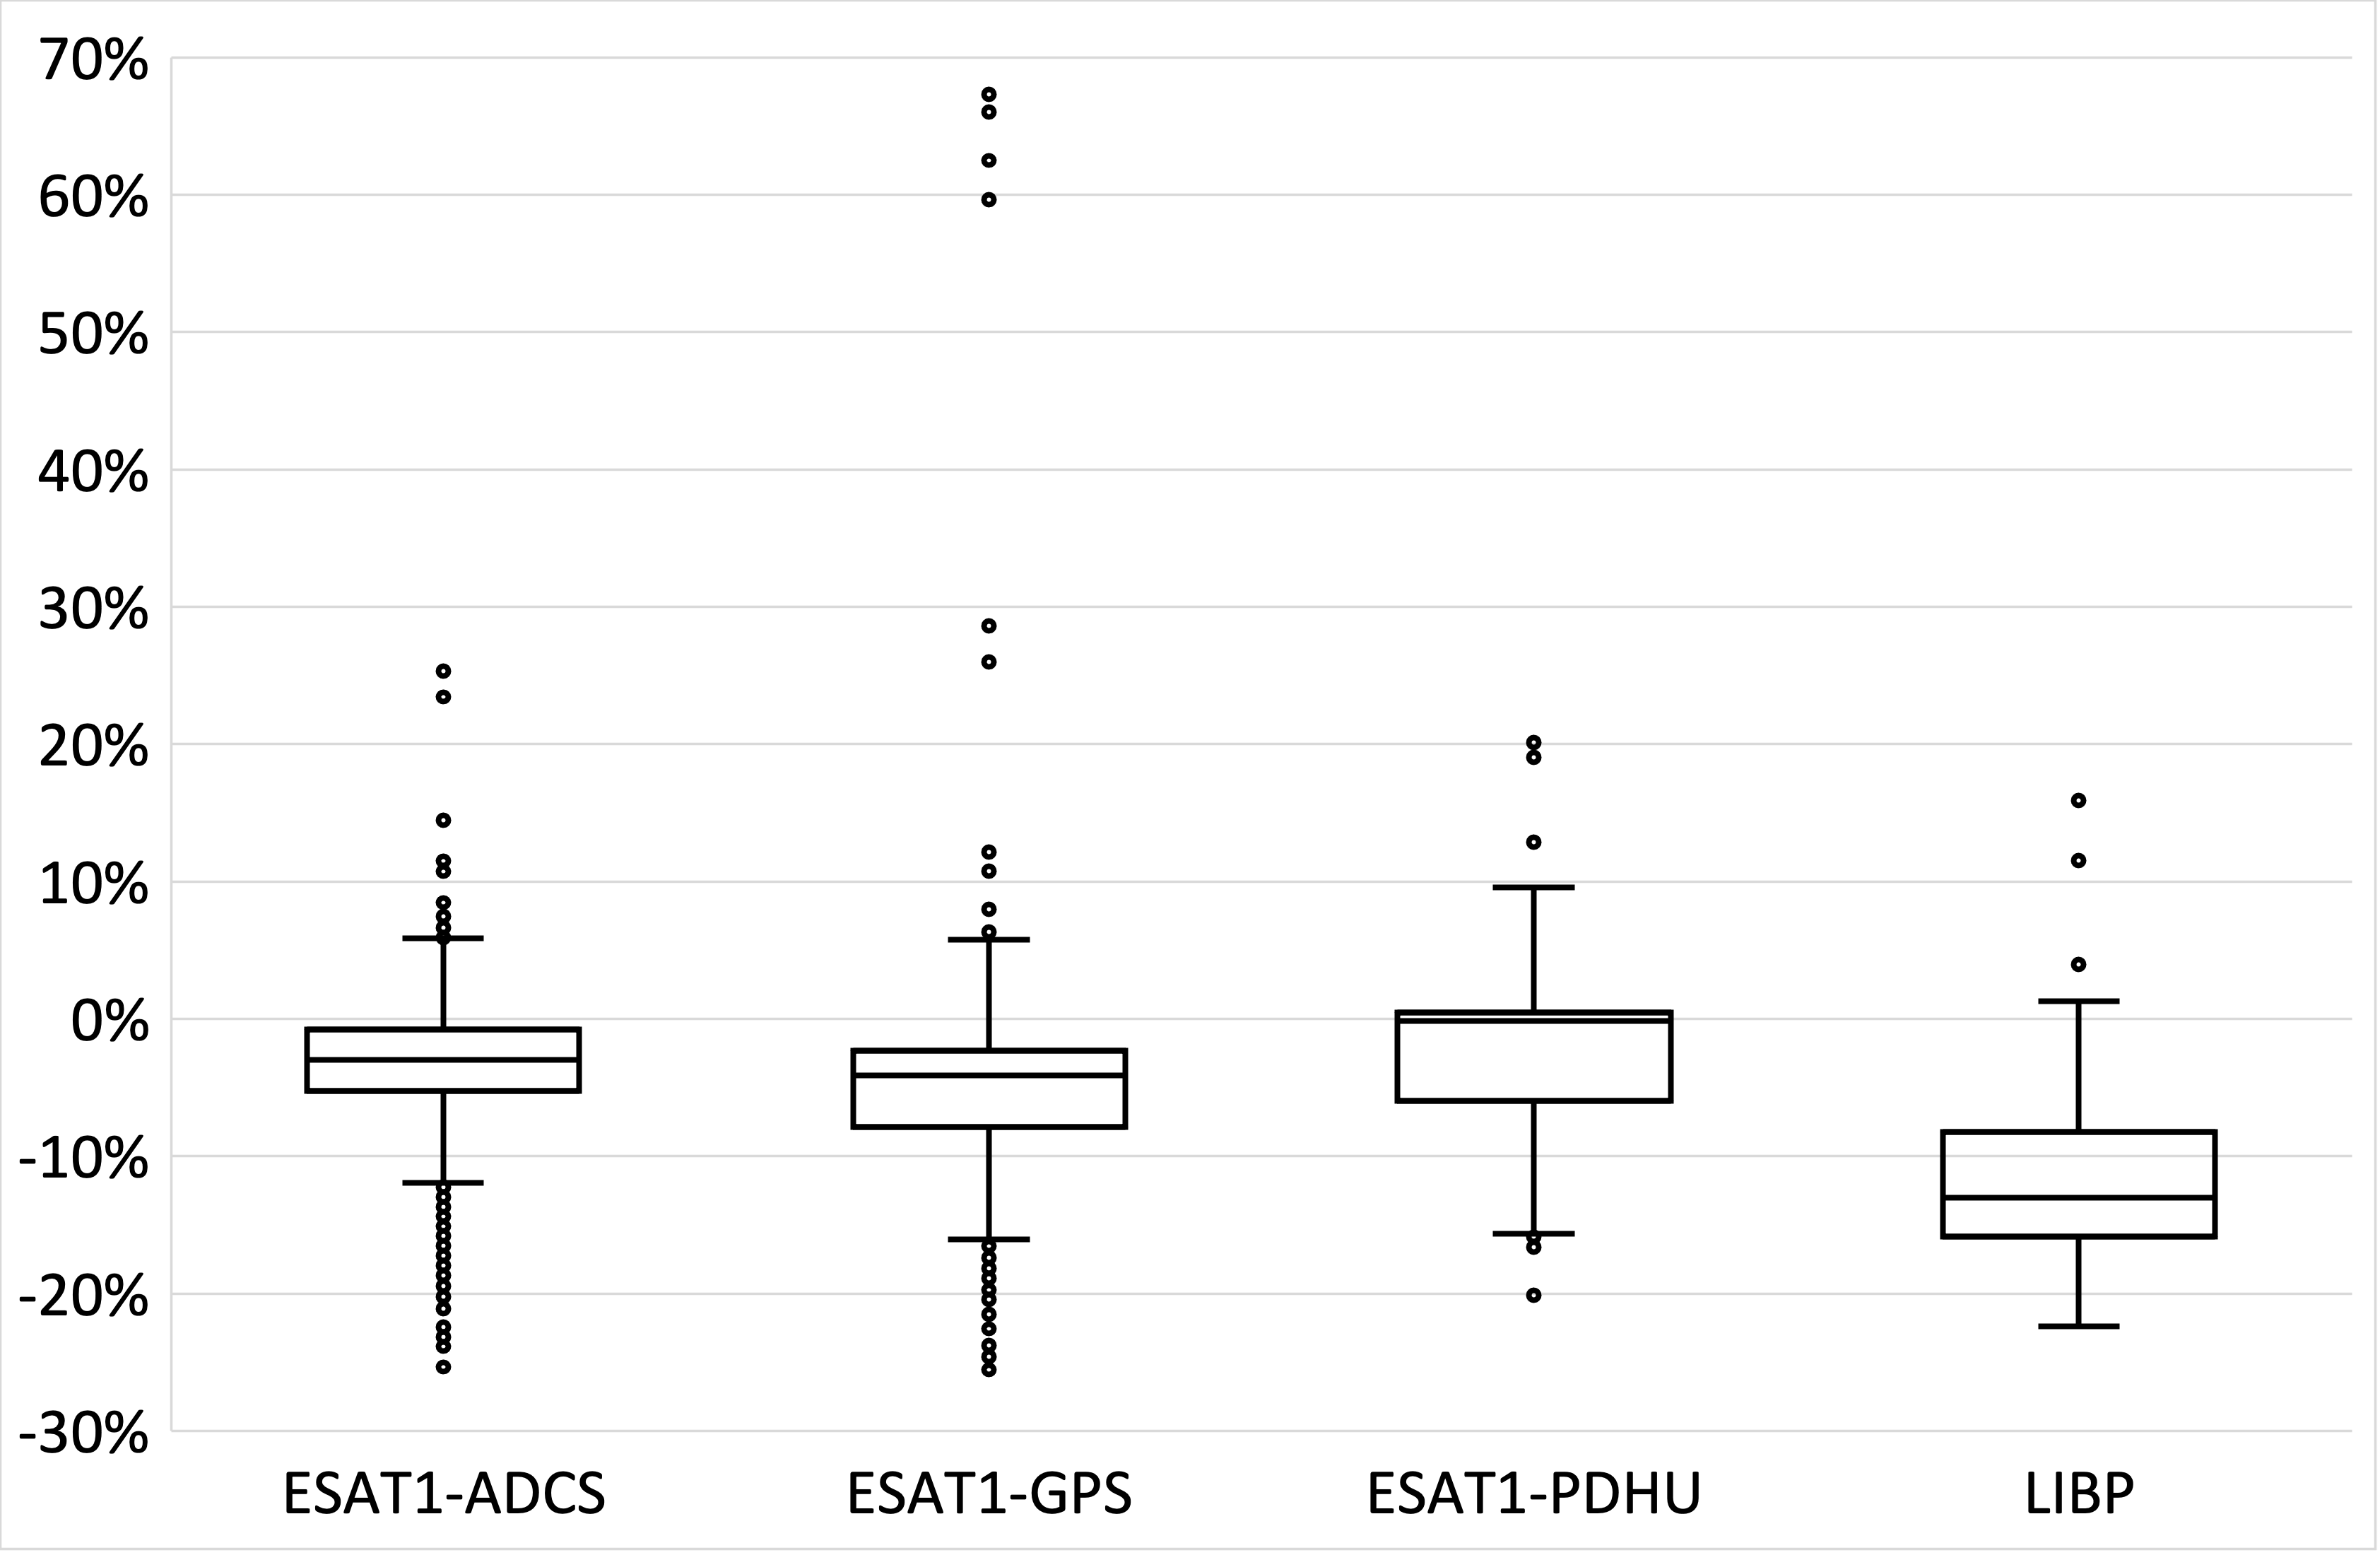
\includegraphics[width=0.8\columnwidth]{DDMA/images/overhead}
%        \caption{\APPR execution overhead per mutant.}
%        \label{fig:appr:overhead}
%    \end{figure}


% \subsection{RQ5 - Relation between data-driven and code-driven mutation analysis}

% \subsubsection*{Design and measurements}

% RQ5 aims to evaluate if data-driven mutation analysis is an alternative to code-driven analysis for a same execution cost (i.e., same number of mutants).
% Particularly, we aim to determine if data-driven mutation analysis subsumes the code-driven one when a same number of mutants is considered. Data-driven mutation analysis subsumes code-driven mutation analysis if
% the set of test cases that achieve maximal mutation analysis results for data-driven mutation analysis achieves the maximal mutation analysis results also for code-driven mutation analysis.
% %every test case that kills a data-driven mutant is guaranteed to also kill a code-driven mutant.

% Since in our context it is not possible to automatically generate 100\% mutation score we assume that the mutation analysis results achieved by the existing test suites are the maximal achievable.

% In practice, we perform an experiment in which we remove all the test cases that kill data-driven mutants and evaluate the effect on the mutation score for the code-driven mutants (hereafter, code-driven mutation score).
% More specifically, (1) we randomly select $N$ code-driven mutants (being $N$ equal to the number of data-driven mutation operations for a specific subject) generated with an extended version of SRCIRor~\cite{hariri2018srciror} from a set of source files targeting the system or sub-system under analysis. 
% (2) We execute the code-driven mutants against the test suite without the test cases killing all data-driven mutants, 
% and (3) we compute the mutation score of such set. 
% If data-driven mutation analysis subsumes code-driven mutation analysis the 
% code-driven mutation score
% shall be close to zero.
% To account for randomness we repeat the experiment 5 times.

% Similarly, we study if code-driven subsumes data-driven mutation analysis by removing all the test cases that kill code-driven mutants and evaluate the effect on the data-driven mutation analysis result. %mutation score for the data-driven mutants.

% On one hand, the nature of code-driven mutation analysis causes the technique to generate a large number of mutants (e.g., hundreds of thousands of mutants~\cite{papadakis2019mutation,zhang2013operator} can be generated for a 70K LoC system), scenario that can be worsened when considering the complexity and size of CPS software, combined with its high test execution cost. 
% On the other hand, data-driven mutation analysis simulates high level faults on interoperability of integrated components, which generates by its nature, a smaller set of mutants (i.e., between 20 and 120 mutants in our subjects).
% Consequently, a reasonable idea would be to consider data-driven mutation analysis rather than code-driven mutation analysis, because of its lower cost.

% To verify the subsumption relation, 

% for each data-driven mutant, we measure the overall number of code-driven mutants non detected when removing the test set killing such data-driven mutant.
% If the resulting distribution of non detected code-driven mutant has an average/median close ($\pm 5\%$) to the total number of originally killed code-driven mutants, means that code-driven mutation was subsumed by data-driven mutation analysis.


% we measure the overall number of code-driven mutants not detected when removing a test case killing a data-driven mutant. If the number is high, it means that data-driven mutation enable to detect more limitations than code-driven mutation.


% To do so, for every subject, and for each data-driven mutant, we remove the test cases that kill the mutant and measure how many code-driven mutants are no longer detected. Then, in a similar way, for each code-driven mutant, we remove the test cases that kill the mutant and measure how many data-driven mutants are no longer detected. 
% When comparing data-driven and code-driven approaches for a specific subject, we consider the same number of mutants (e.g., for the \ADCS subjects we generate 119 data-driven mutants, and 119 code-driven mutants).

% For the assessment of code-driven mutants on our subjects %we use MASS~\cite{}
% we performed the following steps: (1) we used a extended version of SRCIRor~\cite{hariri2018srciror} for the generation of mutants based on the test suite's code coverage, (2) we disregarded equivalent and redundant mutants based on trivial compiler optimizations~\cite{kintis2017detecting}, (3) we randomly sampled $N$ mutants from the whole set and (4) we executed the test suite against the sampled mutants. 

% We study the distribution of the code-driven mutants not detected when removing a test case killing a data-driven mutant. 
% We also study the distribution of the data-driven mutants not detected when removing a test case that kills a code-driven mutant.
% To analyze the distributions we use a t-test that enables the comparison of two distributions. 
% If both distributions have similar means, it indicates that each technique kill a set of mutants that is different from the other approach. In the case that both distribution have different means, it means that one technique kills a set of mutant that includes the set of killed mutants of the other technique.




% \subsubsection*{Results}
% \TODO{TBD}



\subsection{Threats to validity} 


%To ensure the same conditions to all mutant executions, we run each test suite in a clean instance of a virtualized environment.}

\emph{Generalizability}. We have selected industrial software systems of diverse size, tested with different types of test suites. They are developed according to space safety standards and are thus  representative of software system software adhering to safety regulations. Also, \ESAIL is larger than any other industrial system considered in the mutation analysis literature to date~\cite{Ramler2017,delgado2018evaluation,Baker2013,denisov2018mull}.
{\emph{Internal}. To minimize implementation errors, we have extensively tested our toolset; we provide both the test cases and the \APPR source code.}
{\emph{Construct}. The indicators selected for cost estimation (configured operators and LoC) are directly linked to the activities of the end-user and are thus appropriate. We leave empirical studies with human subjects to future work. To discuss overhead, we rely on test execution time, which may be affected by other factors than mutation overhead (e.g., the system behaves differently with mutated data). Dedicated benchmarks might be an alternative.}
{\emph{Conclusion}. To ensure reliability, for RQ1 and RQ2, we confirmed our findings with engineers.}

%However, we realize that the procedure we followed for the selection of pairs of mutants, only showed additional ways to improve and augment a test suite.
%For example, for the \ADCS subject, the procedure showed that two mutants from the same fault model (i.e., SunSensorTM), but targeting different data items, data item 0 and 28 respectively, are failing in the same way. This is not a sign of mutant redundancy, but an evidence that test suite should distinguish the two mutants independently, through two different test cases.
%
%This is in line with related work~\cite{}, showing that test suites should be augmented with additional test cases to make a single mutant fail.


% \subsection{RQ6 - Mutation operation coverage}

% % \subsubsection*{Design and measurements}

% % Given that CPSs are usually constrained by very %strict time limits
% % hard real-time requirements, it may make sense to limit the number of times a mutation probe is activated, to avoid interfering with real-time tasks. 

% % Depending on how often test checks (e.g., test assertions) are performed, it may make sense to reduce the number of times a mutation is performed. For example, short test cases (e.g., unit test cases) often verify every value under test, so even mutating a portion of them might lead to a test fail. 
% % Surely, by reducing the number of times a mutation is performed, we might decrease the chances of a mutant being killed.

% Because of the complexity and size of CPSs, combined with its high test execution cost, we are interested in limiting the number of times a mutation probe is activated.
% To this end, we aim to study how mutation analysis results vary when changing the proportion of data item instances to mutate. 

% % Our goal is to determine the quality of CPS test suites in terms of how often test checks are performed during test suite execution. For instance, a high quality test suite shall detect every mutated data, so in the case that a mutation is applied once, there should be a failing test case.

% Our goal is to provide guidelines for mutants sampling (i.e., the probability of executing a mutant) to determine if there exists a threshold for the sampling rate that makes it likely to detect all the limitations of a test suite.

% To do so, for each subject, we consider the three cases described in Section~\ref{sec:mutantsExecution}:

% \begin{enumerate}
%     \item The mutation is applied only once,
%     for every test case, on the first data item instance processed by the mutation probe.
%     %the mutation occurs the first time the mutant is executed.
%     \item The mutation is applied on every data item instance processed by the mutation probe.
%     \item The mutation is applied with a probability $p$, ranging from 10\% to 90\%, in steps of 10\%.
% \end{enumerate}


% %For each probability $p$ of setup (2), 
% To account for randomness, we repeat the experiment 5 times.
% %, i.e., we compute the mutation score 5 times, based on 5 executions of all mutants against the subject test suite.

% %We discuss the setup that provides the closest mutation score with respect to the mutation score obtained when mutating all the times. 

% We identify the differences between the mutation analysis results obtained across the configurations specified above and assess the significance of such differences.

% \subsubsection*{Results}
% \TODO{TBD}


%% !TEX root = MutationTestingSurvey.tex

\subsection{Run-time Scalability}
\label{sec:opt:execution}

\endinput



If we have $n$ mutants and a test suite of $m$ tests, we have to perform $n \times m$ program executions at maximum.
The main issue remains the scalability of the amount of runnings needed to cover all mutants.

\begin{itemize}
	\item execute only mutants that are reachable by test cases
	\todoinline{easy to reimplement}
	\item is possible to record with one execution all the mutants that can be infected by a test
	\item instead of executing every mutant with every test, it is possible to execute all mutants at once, by monitoring the coverage of the infection conditions
	\item When mutation testing targets strong mutation and the case of test suites take a long execution time, we can reduce the execution time by checking if every mutant achieve weak mutation.
	\todoinline{How easy it is to determine if we have weak mutation in C programs? I think that one of the solutions is linked to split stream.} 
	If weak mutation is not achieved, i.e., if the program state is not infected, there is no point to execute the test case till the end. We can simply report it as not killed and save time.
	\item criticality: since determining whether a test execution can terminate or not is an undecidable problem, heuristic solutions are needed. Such as establishing time thresholds for running executions.
	\todoinline{but if we face this problem, isn't it enough to check if a test execution is taking twice the expected time? I mean, if the test case does not fail in 3 times the original execution time we can report the mutant as not killed. But the solution to this problem might be to add a timeout inside the test suite.}
	\item take advantage of common executions parts (between the original program and mutants). Called as Split-Stream execution
\end{itemize} 

Strong, weak and firm mutation
\begin{itemize}
	\item Strong mutation:
	\item Weak mutation: the mutant is killed if any mutated component changes its state (variable reference, variable assignment, arithmetic expression, relational expression, boolean expression). Advantages: weak mutation does not need a complete execution. Cons: sacrifices test effectiveness with test effort.
	\item Firm mutation: the killing process occurs between weak and strong mutation
\end{itemize} 

Runtime optimization techniques
\begin{itemize}
	\item Interpreter based technique: results are analysed from the source code
	\item Compiler based technique: results are analysed from the execution of binary code 
	\todoinline{how much gain can it give?}
	\item Mutant Schema Generation: creates a metaprogram, there is research on mutating bytecode
	\todoinline{Does MUSIC implement it? We can implement it as a postprocessing. We compare files generated by MUSIC. We identify the changed lines (mutants). Then we generate a single file where we have options for each changed line.}
\end{itemize}

\input{reduceprioritise}


%
%% !TEX root = MutationTestingSurvey.tex

\subsection{Solutions to Improve Compile-time Scalability}
\label{sub:compileTime}
\label{sec:opt:selection}

Another source of \INDEX{scalability issues} is the compilation of mutants;
indeed, because of the large number of mutation operators available in the literature, the number of mutants to be compiled is not negligible. In this section we report the main research results aiming at reducing the time required to compile mutants.
%has worked on approaches based on optimising the compilation process.

Untch et al. \cite{untch1993mutation} proposed a technique called \INDEX{mutant schemata}; the technique introduces the concept of meta-program, which stands for including and compiling all the mutants in a single executable file, instead of compiling one executable per mutation generated. The mutations are then managed at run-time through parameters that enable software engineers to choose the mutation to be executed, results show speed improvements over 300\% \cite{untch1993mutation,papadakis2010automatic}. Modern mutation testing tools such as Accmut \cite{wang2017faster} and Milu \cite{jia2008milu} include this type of optimisation.

Another solution consists of mutating directly the compiled code so that mutants can be executed without compiling each of them.
This optimisation has been applied on 
Assembly languages \cite{crouzet2006sesame},
Java bytecode \cite{ma2006mujava}, 
binary code for embedded software \cite{becker2012xemu},
Common Intermediate Language (.NET) \cite{derezinska2011object} 
and LLVM IR \cite{hariri2016evaluating}. 
Results obtained by Derezinska and Kowalski \cite{derezinska2011object} show that, on average, the mutation testing process mutating compiled code requires only 50\% of the time required by a traditional mutation testing process applied to source code. 
Additionally, the mutations performed on compiled code can be applied directly to multiple source languages (e.g., LLVM IR supports C, C++, Objective-C, Objective-C++, OpenMP, OpenCL and CUDA) \cite{hariri2019comparing}.
However, there are some drawbacks when mutating compiled code, for example many of the mutations generated cannot be represented at the source code level \cite{jia2010analysis}, creating not relevant mutations. 
In the case of mutation of binary code, the mutation process can become very expensive since it is necessary to translate the code into machine readable instructions \cite{becker2012xemu}.




%
%% !TEX root = MutationTestingSurvey.tex

\subsection{Equivalent Mutants}
\label{sec:opt:equivalent}

Equivalent mutants are mutants that behave as the original program, they are semantically equivalent to the original version despite being syntactically different. Equivalent mutants are an actual problem that can lead mutation testing to be infeasible, Schuler and Zeller \cite{schuler2013covering} showed that 45\% of not killed mutants are equivalent, and that manually checking if a mutant is equivalent can take on average up to 15 minutes. Even though, the process of identifying equivalent mutants has been defined as an undecidable problem \cite{madeyski2013overcoming}, the research has cope with heuristics to tackle this issue.

According to the literature \cite{madeyski2013overcoming}, the equivalent mutant heuristics can be classified in two different groups: (1) detecting equivalent mutant techniques, and (2) reducing equivalent mutant techniques.

\subsubsection{Detecting Equivalent Mutant Techniques}

The first group aims to detect and discard the equivalent mutants during the mutation process. In this direction, Papadakis et al. \cite{papadakis2015trivial, kintis2017detecting,papadakis2019mutation} has developed the Trivial Compiler Optimisation technique, the approach relies on the idea that compiler optimisations transforms mutants to the optimised version, thus when the original program can be transformed by an optimisation to one of its mutants, then the mutant is defined equivalent.
Recent studies \cite{papadakis2015trivial} show that the Trivial Compiler Optimisation is able to detect approximately up to 30\% of the equivalent mutants.

A different approach for detecting equivalent mutants is to formulate the problem as a constraint satisfaction problem. The main idea is to analyze the path condition of a mutant, in which the mutant is defined equivalent if and only if the input constraint is unsatisfiable. Offutt et al. \cite{offutt1996detecting,offutt1997automatically} carried out an experimental evaluation on 11 Fortran subject programs and detected 47\% of the existing equivalent mutants by applying this heuristic.
Similarly, Holling et al. \cite{holling2016nequivack,papadakis2012mutation} presented an approach for identifying non-equivalent mutants and improving the confidence of the mutation score. By using static analysis and symbolic execution they defined a six-steps procedure to determine which mutants are \textit{non-equivalent}. \textit{Non-equivalent} mutants are identified every time they find a counter-example input for which the outputs of a pair of functions (the original function and the mutant one) is different. In the case no counter-example is found, then the mutant is classified as \textit{unknown}. 
In like manner, Riener et al. \cite{riener2011test} proposed the Symbolic Bounded Model Checking (SymBMC) procedure for the automated generation of test cases from a set of mutants. The approach examines the original program and its mutants on the same input and seeks for executions resulting in different observable output for the program and mutants, if the procedure finds a failing execution, the input data is saved as an effective new test case. Every time a new test case is found, the mutant is defined as non-equivalent, in a similar way to Holling's approach \cite{holling2016nequivack}.

Other approaches consider the use of software clones (i.e., similar code fragments) to detect equivalent mutants \cite{kintis2013identifying}, in this work Kintis proposed that mirrored mutants (i.e., mutants that belong to the same software clone) present the same behavior with respect to each other. So, for a set of mirrored mutants, is enough to prove equivalence of one mutant, instead of trying to detect equivalence for the whole set.

With a different approach, Adamopoulos et al. \cite{adamopoulos2004overcome} introduced a co-evolutionary technique for detecting equivalent mutants. The technique defines a fitness function that sets a poor fitness value to an equivalent mutant. Through the fitness function equivalent mutants are removed during the co-evolutionary process, and only mutants that are hard to kill and test cases that are good at detecting mutants are kept for future iterations of the algorithm. On the other hand, Maldonado et al. \cite{maldonado2005bayesian} developed a Bayesian Learning-Based technique for helping tester to detect equivalent mutants using an inference algorithm.

% 	\item Margrave's change-impact analysis \cite{martin2007fault} (READ)
% 	\item Using Lesar model-checker for eliminating equivalent mutants \cite{du2008towards} (READ)

% \textbf{Avoiding equivalent mutant generation techniques}

% \begin{itemize}
% 	\item \textbf{Selective mutation} \cite{mresa1999efficiency}:
% 	Randomly selecting 10\%, 20\%, 30\%, 40\%, 50\% and 60\% of the mutants results in a fault loss of approximately 26\%, 16\%, 13\%, 10\%, 7\% and 6\% respectively \cite{papadakis2010empirical}.

\subsubsection{Reducing Equivalent Mutant Techniques}

The second group of techniques aims to reduce the amount equivalent mutants produced during mutation process.
In this direction, Gr\"{u}n et al. \cite{grun2009impact} proposed that mutants that do not alter the dynamic control-flow with respect to the original program, should be avoided since they have a greater chance of being equivalent. To measure the dynamic control-flow difference (i.e., the impact), they defined the impact as the number of classes with different statement coverage. On the empirical evaluation performed on JAXEN (12,449 LOC), by analyzing the mutants that were covered by the test bench but not killed, they performed several experiments with two main results. 
The first result was about the relation between impact on control-flow and likelihood of the mutant of being non-equivalent, the experimental results were obtained by randomly selecting 20 mutants, they discovered that the 60\% of the mutants with control-flow impact were classified as non-equivalent, and that the 60\% of the mutants without control-flow impact were classified as equivalent. 
The second result was about the relation between the impact on control-flow degree and likelihood of the mutant of being non-equivalent, the results were obtained by analyzing two specific subsets (e.g., (a) subset with the 20 mutants with highest impact, and (b) subset with the 20 mutants with lower impact), from the first subset with higher impact, 90\% of the mutants were non-equivalent, while on the second subset 55\% were equivalent mutants. The conclusion is that testers can effectively focus on mutations with higher impact, at the expense of loosing mutations that could reveal another type of faults.

In the same research line, Schuler et al. \cite{schuler2009efficient} demonstrated that mutants that violate dynamic invariants (i.e., invariants derived from data collected using dynamic analysis) are less likely to be equivalent and should be preferred over those that do not alter invariants with respect to the original program version. In an empirical evaluation performed on JAXEN, they analyzed two subset of mutants (e.g., (a) 12 random mutants that do not violate invariants, and (b) 12 mutants with highest score of invariants violated during execution), the results indicate that from the violating mutants 83\% were non-equivalent, while from the non-violating mutants only 33\% were non-equivalent.

A different perspective is to focus in code coverage of mutants, for example, Schuler et al. \cite{schuler2010covering,schuler2013covering} discovered that mutants that change code and data coverage with respect to the original program, has a likelihood of 68\%-79\% to be non-equivalent.
On an empirical evaluation performed on 140 mutations from seven open-source projects, the authors discovered (1) that operators that modify the control-flow such as \textit{negate jump condition} or \textit{omit method call} produce less equivalent mutants (30\%) than operators that only change data (57\%), and (2) that from several metrics based on differences in statement (i.e., number of methods that have at least one statement that is executed at a different frequency between mutated and original program) and data (i.e., number of methods that have at least one different return value between mutated and original program) coverage, the authors discovered that by measuring both impact on data and code coverage is possible to obtain few false negative results (61\%) when assessing if a mutant is equivalent or not, in comparison with measuring data and code coverage independently (56\% and 67\% ,respectively).

Program slicing has been presented as a possible mechanism for reducing equivalent mutants \cite{voas1997software, hierons1999using, harman2001relationship}: in particular, Harman et al. \cite{harman2001relationship} presented a technique for reducing equivalent mutation generation using program dependence analysis. The idea is to avoid mutants that fail to propagate corrupted data into the inspection set at the probe point, a mutant that fails to propagate specific data means that no semantic change is being introduced on the software behavior. To carry on this analysis, the authors used a method called \textit{JR-dependence}, the method allows to relate variable and node pairs rather than simply considering nodes. With \textit{JR-dependence} is possible to know the set of variables that can and cannot be used to kill a mutant, which is beneficial for mutation testing. 
Consequently, Offutt et al. \cite{offutt2006class} used the guidelines by Harman et al. \cite{harman2001relationship} to eliminate equivalent mutants by applying the optimizations directly in the implementation of object oriented operators developed on the MuJava mutation testing tool. 

On the other hand, Kintis et al. \cite{kintis2014using,kintis2015medic} discovered that through static data-flow analysis is possible to reveal code locations that are sensitive to produce equivalent mutants together with the mutation operators being applied. The first pattern is called \textit{Use-Def} Problematic Pattern and seeks for uses of variables that reach a definition and can be mutated by a mutation operator that produces in-place changes (e.g., $\{x = (m + x)/2\}$ mutate to $\{x = (m + x++)/2\}$), specifically this pattern can be applied on definitions at the same line, basic block and between different basic blocks. The second pattern is called \textit{Def-Def} Problematic Pattern and seeks for subsequent definitions of a certain variable, in other words, if a definition reach another definition of the same variable without a prior use of the variable, then any mutation to the first definition cannot be revealed since its being redefined. On the experimental evaluation guided on 6 real-world programs, the technique was able to automatically detect 58 out of 84 equivalent mutants, leaving only a 30\% of mutants to be analyzed manually.

Research has proved that higher order mutation testing can be helpful in reducing equivalent mutants \cite{jia2009higher,kintis2010evaluating,offutt1992investigations,papadakis2010empirical}, since two or more mutations are applied simultaneously, the chances of producing equivalent mutants decreases consistently. For instance, Papadakis and Malevris \cite{papadakis2010empirical}, worked on a approach for higher order mutants for the C programming language that lead to a reduction of approximately 80-90\% of the generated equivalent mutants, with a fault detection ability loss only of 11-15\%. 
% For instance, Offutt demonstrated that the set of test data developed for first order mutants (FOMs) actually killed a higher percentage of mutants when applied to second order mutants (SOMs) \cite{offutt1992investigations}. 
% Jia and Harman identified six different types of HOMs \cite{jia2009higher} and presented a categorization of HOMs. They introduced the concept of subsuming and strongly subsuming HOMs.
% Polo et al. \cite{polo2009decreasing} studied three strategies to combine FOMs and generate mutants, and found that they can achieve significant cost reductions without losing any effectiveness (they reduced the number of mutants in a approximately 50\%, without much decrease in the quality of the test suite).
%Instead, Kintis et al. \cite{kintis2010evaluating} developed a solution for the Java language, they state that SOMs achieve higher collateral coverage for strong mutation as compared with third or higher order mutants. With their approach they obtained a mutant reduction of between 65-87\% and a loss of test effectiveness from 1.75-4.2\%.
% Mateo et al. \cite{mateo2012validating,madeyski2013overcoming} found that second order mutants (SOM) are significantly more efficient that first order mutants (FOM).

\endinput

\begin{table*}[ht]
\centering
\scriptsize
\begin{tabular}{lllllllp{4cm}}
\toprule
Author(s)          & Year   & Language & \begin{tabular}[c]{@{}l@{}}Largest\\Subject\end{tabular} & \begin{tabular}[c]{@{}l@{}}\#Eq. \\ Mutants\end{tabular} & \begin{tabular}[c]{@{}l@{}}Available \\ Tool\end{tabular} & Category                                                 & Findings                                                                                      \\
\midrule
Baldwin \& Sayward \cite{baldwin1979heuristics} & 1979   &          &                                                           &                                                          &                                                           & Detect                                                   & Compiler optimization can be used to detect equivalent mutants                                \\
Acree  \cite{acree1980mutation}       & 1980   & Fortran  &                                                           & 25                                                       &                                                           & Detect                                                   & Human make mistakes when they identify equivalent mutants                                     \\
Offutt \& Craft \cite{offutt1994using}   & 1994   & Fortran  & 52                                                        & 255                                                      &                                                           & Detect                                                   & Compiler optimisation can detect on average 45\% of equivalent mutants                        \\
Offutt \& Pan \cite{offutt1996detecting,offutt1997automatically}     & 1996-7 & Fortran  & 29                                                        & 695                                                      & Yes                                                       & Detect                                                   & Constraint-based testing can detect on average 47\% of equivalent mutants                     \\
Voas \& McGraw \cite{voas1997software}    & 1997   &          &                                                           &                                                          &                                                           & Detect                                                   & Slicing may be helpful in detecting equivalent mutants                                        \\
Hierons et al. \cite{hierons1999using}      & 1999   &          &                                                           &                                                          &                                                           & \begin{tabular}[c]{@{}l@{}}Detect/\\ Reduce\end{tabular} & Program slicing can be used to detect and assist the identification of equivalent mutants     \\
Harman et al.  \cite{harman2001relationship}    & 2001   &          &                                                           &                                                          &                                                           & \begin{tabular}[c]{@{}l@{}}Detect/\\ Reduce\end{tabular} & Dependence analysis can be used to detect and assist the identification of equivalent mutants \\
Adamopoulos et al  & 2004 \cite{adamopoulos2004overcome}  &          &                                                           &                                                          &                                                           & Reduce                                                   & Co-evolution can help in reducing the effects of equivalent mutants                           \\
Grun et al. \cite{grun2009impact}       & 2009   & Java     & 12,449                                                     & 8                                                        & Yes                                                       & Reduce                                                   & Coverage Impact can be used to classify killable mutants                                      \\
Schuler et al. \cite{schuler2009efficient}    & 2009   & Java     & 94,902                                                     & 10                                                       & Yes                                                       & Reduce                                                   & Invariants violations can be used to classify killable mutants                                \\
Schuler \& Zeller \cite{schuler2010covering,schuler2013covering} & 2010-2 & Java     & 94,902                                                     & 63                                                       & Yes                                                       & Reduce                                                   & Coverage impact can be used to classify killable mutants                                      \\
Nica \& Wotawa \cite{nica2012using}    & 2012   & Java     & 380                                                       & 1,424                                                     &                                                           & Detect                                                   & Constraint-based testing can detect equivalent mutants                                        \\
Kintis et al. \cite{kintis2012isolating,kintis2015employing}     & 2012-4 & Java     & 94,902                                                     & 89                                                       &                                                           & Reduce                                                   & Higher order mutants can be used to classify killable mutants                                 \\
Kintis \& Malevris \cite{kintis2014using} & 2014   & Java     & 25,909                                                     & 84                                                       &                                                           & Detect                                                   & Data-flow patterns can detect 69\% of the equivalent mutants introduced by the AOIS operator  \\
Papadakis et al. \cite{papadakis2014mitigating}    & 2014   & C        & 513                                                       & 5,589                                                     &                                                           & Reduce                                                   & Coverage impact can be used to classify killable mutants                                      \\
Papadakis et al. \cite{papadakis2015trivial}    & 2014   & C        & 362,769                                                    & 9,551                                                     & Yes                                                       & Detect                                                   & Compilers can be used to effectively automate the mutant equivalence detection               \\
\bottomrule
\end{tabular}
\end{table*}


%
%% !TEX root = MutationTestingSurvey.tex

\subsection{Solutions to Minimize Redundant Mutants}
\label{sec:opt:redundant}

The term \INDEX{redundant mutant} is used to refer to mutants that show the same behaviour of other mutants, i.e., they
are killed every time other mutants are also being killed. 
%Redundant mutants are another particular category of mutants, these mutants do not contribute to the testing process, since they are killed every time other mutants are also being killed. 
\emph{The main drawback of redundant mutants is that they can artificially inflate the apparent ability of a test technique to detect faults, in other words they tend to skew the mutation score measurement leading to serious threats to the validity of empirical research}~\cite{papadakis2016threats}.

%\DONE{Is it possible to add an example?}

\input{listings/redundants}

In Section~\ref{sec:process} we introduced a mutation testing example for the function \texttt{isPalindrome}. 
Listing~\ref{redudantexample1} and~\ref{redudantexample2} show excerpts from mutants \textit{M4} and \textit{M5} obtained with the \textit{SSDL} operator. In this case, both mutants are considered not equivalent with respect to the original program, but they are redundant between each other, because they are being killed by the same test cases, that is, the test cases exercising the inputs \texttt{abba} and \texttt{aba}.
\REVTWO{C32}{In this case, the solution to the problem is dual. The first solution accounts for introducing one new test case that should produce different outputs for both mutants, which in this case is infeasible since there is no test case able to produce different output for mutants in Listing~\ref{redudantexample1} and~\ref{redudantexample2}. The second solution consists of excluding randomly one of the two mutants.}

%\DONE{The following sentence is not good. Can we say something more, for example how many SUT they considered, which mutation operators they considered?}

To highlight that redundant mutants are a recurrent problem, Kintis et al.~\cite{kintis2010evaluating} showed in an experiment that 9\% of mutants were redundant. For the experimental evaluation the authors considered 15 SUT, on a total of 372 LOC, and 6\,127 test cases, and applied the sufficient set of operators for generating the mutants. 

\MREVISION{C15}{Identifying all the redundant mutants is equal to finding the minimal set of mutants. \textit{A minimal set of mutants has no redundancy, that is, every test set that kills these mutants will also kill all remaining mutants}~\cite{kurtz2015static}.} 
%Similar to the case of equivalent mutants, finding the minimal set of mutants is an undecidable problem, and it can be only approximated.}

%\DONE{The definition below is not clear. I cannot understand teh difference between them}
In the literature, redundant mutants are divided into two categories. The first is the category of \INDEX{duplicated mutants}, that is, mutants that are equivalent with each other but not equivalent to the original program. The second category concerns \INDEX{subsumed mutants}, that is, mutants that are not equivalent with each other but are killed by the same test cases. 
\MREVISION{C15}{Only duplicate mutants are a problem for test suite evaluation; indeed, subsumed mutants are mutants that capture different faults. Unfortunately, automatically distinguishing the two cases is not feasible since it reduces to the problem of automatically identifying duplicated mutants, which, in turn, coincides with the problem of identifying equivalent mutants. Often, automated techniques simply identify mutants that lead to the same test failures, i.e., both duplicated and subsumed mutants.}

Previous studies showed redundancies between mutation operators and proved that a certain subset of operators is sufficient to measure test effectiveness. For instance, Rothermel et al.~\cite{rothermel1996experimental} and then Andrews et al.~\cite{andrews2005mutation} proposed a small set of operators that is lead to a sufficiently accurate approximation of the results obtained by using all possible operators (e.g., replace numerical constant, negate jump condition, replace arithmetic operator, omit method calls). In the same direction, Namin et al.~\cite{siami2008sufficient} proposed a statistical analysis procedure for identifying a subset of operators that could predict mutation score, their approach reduced mutants in a 93\% on C programs. 

More recently, Delamaro et al.~\cite{delamaro2014designing} designed deletion operators, and found that they form a cost-effective alternative to other operators, i.e., they produce less redundant mutants. The deletion operator by itself has been proven to be the most effective for fault detection~\cite{delamaro2014designing}.

%With a different perspective, 
Papadakis and Malevris~\cite{papadakis2012mutation} and then Kurtz et al.~\cite{kurtz2015static} proposed a path selection strategy (i.e., they generate new test inputs) for selecting the test cases able to effectively kill mutants using \INDEX{symbolic execution}, and to consequently decrease the number of redundant mutants. 
The authors suggest constrained versions of the logical, relational and unary operators for generating less redundant mutants. 
In a similar manner, Just et al.~\cite{just2012redundant,just2015higher} proved that these three operators are better at detecting faults that the rest of mutation operators.

Delgado et al.~\cite{delgado2017assessment} show that some operators naturally produce more redundant mutants than others and
developed a selective approach for reducing the number of mutants without loss of effectiveness for C++ programs. 

The approach introduces a degree of redundancy for every mutation operator that helps developers to choosing the mutation operators with a lower degree of redundancy, based on the test cases defined in the project.

Another solution to reduce the number of redundant mutants is the application of trivial \INDEX{compiler optimisations}~\cite{papadakis2015trivial, kintis2017detecting,papadakis2019mutation}. 
It can identify duplicate mutants by comparing the optimised object code of each mutant. The empirical study guided by Kintis et al.~\cite{kintis2017detecting} showed that by using compiler optimisations it is possible to reveal 21\% and 5.4\% of C and Java mutants, respectively.


Finally, Shin et al. suggest to avoid discarding redundant mutants but, instead, augment the test suite with additional test cases so that 
each mutant can trigger a test failure that cannot be observed with other mutants~\cite{Shin:TSE:DCriterion:2018}. 
They introduce the \INDEX{distinguishing mutation adequacy criterion} to characterize test suites in which every mutant triggers a test failure that is not observed with other mutants.
Empirical results show that test suites that satisfy the distinguishing mutation adequacy criterion have a higher
 fault detection effectiveness than test suites that simply satisfy mutation coverage.





%% !TEX root = MutationTestingSurvey.tex

\subsection{Mutation Score Calculation}
\label{sub:mutationscore}

%\DONE{Is there anything we can add here?}

\MREVISION{C6}{The \INDEX{mutation score} captures, in percentage points, the quality of a test suite. It measures the percentage of mutants that had been killed by the test suites.} 
The mutation testing process is driven by the mutation score; the process iterates multiple times until the mutation score reaches a certain threshold. 

According to recent studies, there is a relation between the mutation score and the fault revelation ability of mutation testing.
\MREVISION{C7}{A recent empirical evaluation, for example, has shown that \textit{achieving high mutation scores improves significantly the fault detection capability of a test suite}
~\cite{papadakis2018mutation}. 
\DONE{The following sentence is incomplete. You cannot say "similar fault detection ability that statement and branch coverage". Do you mean 100\% branch coverage (i.e., branch adequate)? Also putting together branch and statement is tricky, because branch is a stronger criterion. }
This evaluation shows that a test suite that reaches a mutation score of 80\% has a similar  similar fault detection capability of one that achieves 80\% branch coverage. 
\DONE{Why do we have to put both 90 and 95?}
Instead, a test suite that reaches a mutation score of 90\% outperforms this code coverage criterion. The drawback of this result, is, however, that the fault detection ability of mutation testing is high only with a high mutation score.}

%To reliably compute the mutation score it is necessary to identify equivalent and redundant mutants. 
As seen in Section~\ref{sec:opt:equivalent} and~\ref{sec:opt:redundant}, equivalent and redundant mutants can affect (i.e., cause an overestimation or underestimation) the mutation score~\cite{papadakis2016threats,kintis2017detecting}.
Hence, it is desirable to identify the presence of such mutants before estimating the fault revelation ability of a test suite.


% !TEX root = MAIN.tex
\clearpage
\section{Code-driven Mutation Testing (Test Suite Augmentation)}
\label{sec:testGeneration:codeDriven}

\subsection{Overview}

We address the following research questions:

\emph{RQ1. Does SEMuS scale in the context of space software?}

\emph{RQ2. Does SEMuS improve the mutation score of test suites?}

\subsection{Subjects of the Study}

To perform our experiments, we considered two software artifacts, both of them provided by the European Space Agency (ESA): ASN1SCC (or ASN.1) and MLFS.
In the case of ASN.1, the test suite is automatically generated with an approach that aims to maximize the boundary conditions of the input domain being covered. 
The Mathematical Library for Flight Software (MLFS) implements mathematical functions qualified for flight software (it complies with ECSS criticality category B).
Both test suites considered in this study characterize by high statement coverage as required by space software standards (e.g., category C software requires statement adequacy according to ECSS). MLFS test suite achieves MC/DC coverage (i.e., 100\% coverage), while ASN.1 case study achieves 99\% statement coverage.

% \TODO{to be fixed}
% \REVOCT{C-P-19}{We did not considered ESAIL in our empirical evaluation, because of the known incompatibility of clang (i.e., the compiler required by SEMuS) and ESAIL specific compilation libraries (i.e., RTEMS). More details can be found in Section~\ref{}.}

\subsection{Setup}

To address our research questions, we consider mutation analysis a precondition for our subjects; this is necessary since test generation only requires the list of live mutants (i.e., generating test inputs for all possible mutants would be far too expensive). Table~\ref{table:results:semus:ms} reports the mutation analysis results (i.e., MASS output) for the ASN.1 and MLFS subjects.

\begin{table}[htb]
\caption{Mutation scores for artifacts.}
\label{table:results:semus:ms} 
\centering
\begin{tabular}{|
@{\hspace{1pt}}p{20mm}|
@{\hspace{1pt}}>{\raggedleft\arraybackslash}p{20mm}@{\hspace{1pt}}|
>{\raggedleft\arraybackslash}p{15mm}@{\hspace{1pt}}|
>{\raggedleft\arraybackslash}p{15mm}@{\hspace{1pt}}|
 >{\raggedleft\arraybackslash}p{35mm}@{\hspace{1pt}}|
}
\hline
\textbf{Subject}&\textbf{Mutants}&\textbf{Killed}&\textbf{Live}&\textbf{Mutation Score (\%)}\\ 
\hline
$\mathit{MLFS}$&21\,375&17\,484&3\,891&81.80 \\
$\mathit{ASN.1}$&5\,323&3\,104&2\,219&58.31 \\
\hline
\end{tabular}

\end{table}

As shown in Table~\ref{table:results:semus:ms}, we apply test generation for the 3\,891 live mutants of MLFS, and for the 2\,219 live mutants of the ASN.1 subject.
For every subject, we applied the SEMuS toolset on Linux OS running on the HPC cluster of the University of Luxembourg. The HPC cluster consists of Intel Xeon E5-2680 v4 (2.4 GHz) nodes. To make our experiments feasible we executed 14 SEMuS parallel instances running on a dedicated node.

\subsection{RQ1 - Approach scalability}
\label{sec:rq1:semus}

To assess \INDEX{SEMuS} scalability we measure the execution time of each SEMuS instance. Table~\ref{table:results:semus:times} shows statistics about execution times for MLFS and the ASN.1 subjects.
Firstly, we notice is that median time taken by SEMuS to generate test inputs is the same for both case studies (i.e., 0.4 minutes). While, the mean differs for both case studies, 8.5 minutes for MLFS, and 33.4 for ASN.1 case study. Secondly, we notice that the maximum execution time is limited by the configuration we imposed in SEMuS for the symbolic search, that is, two hours.
Lastly, we notice that the total execution time of MLFS is approximately 556 hours, which can be executed on only 5.5 hours if executed with 100 HPC nodes. Similarly, the ASN.1 subject can be executed in approximately 1\,161 hours, or 11.6 hours if executed with 100 HPC nodes. In this context, even paying for the computational power of 100 HPC nodes for making test generation feasible in half a day is economically justifiable in the space software context.

    \begin{figure}[tb]
    \centering
        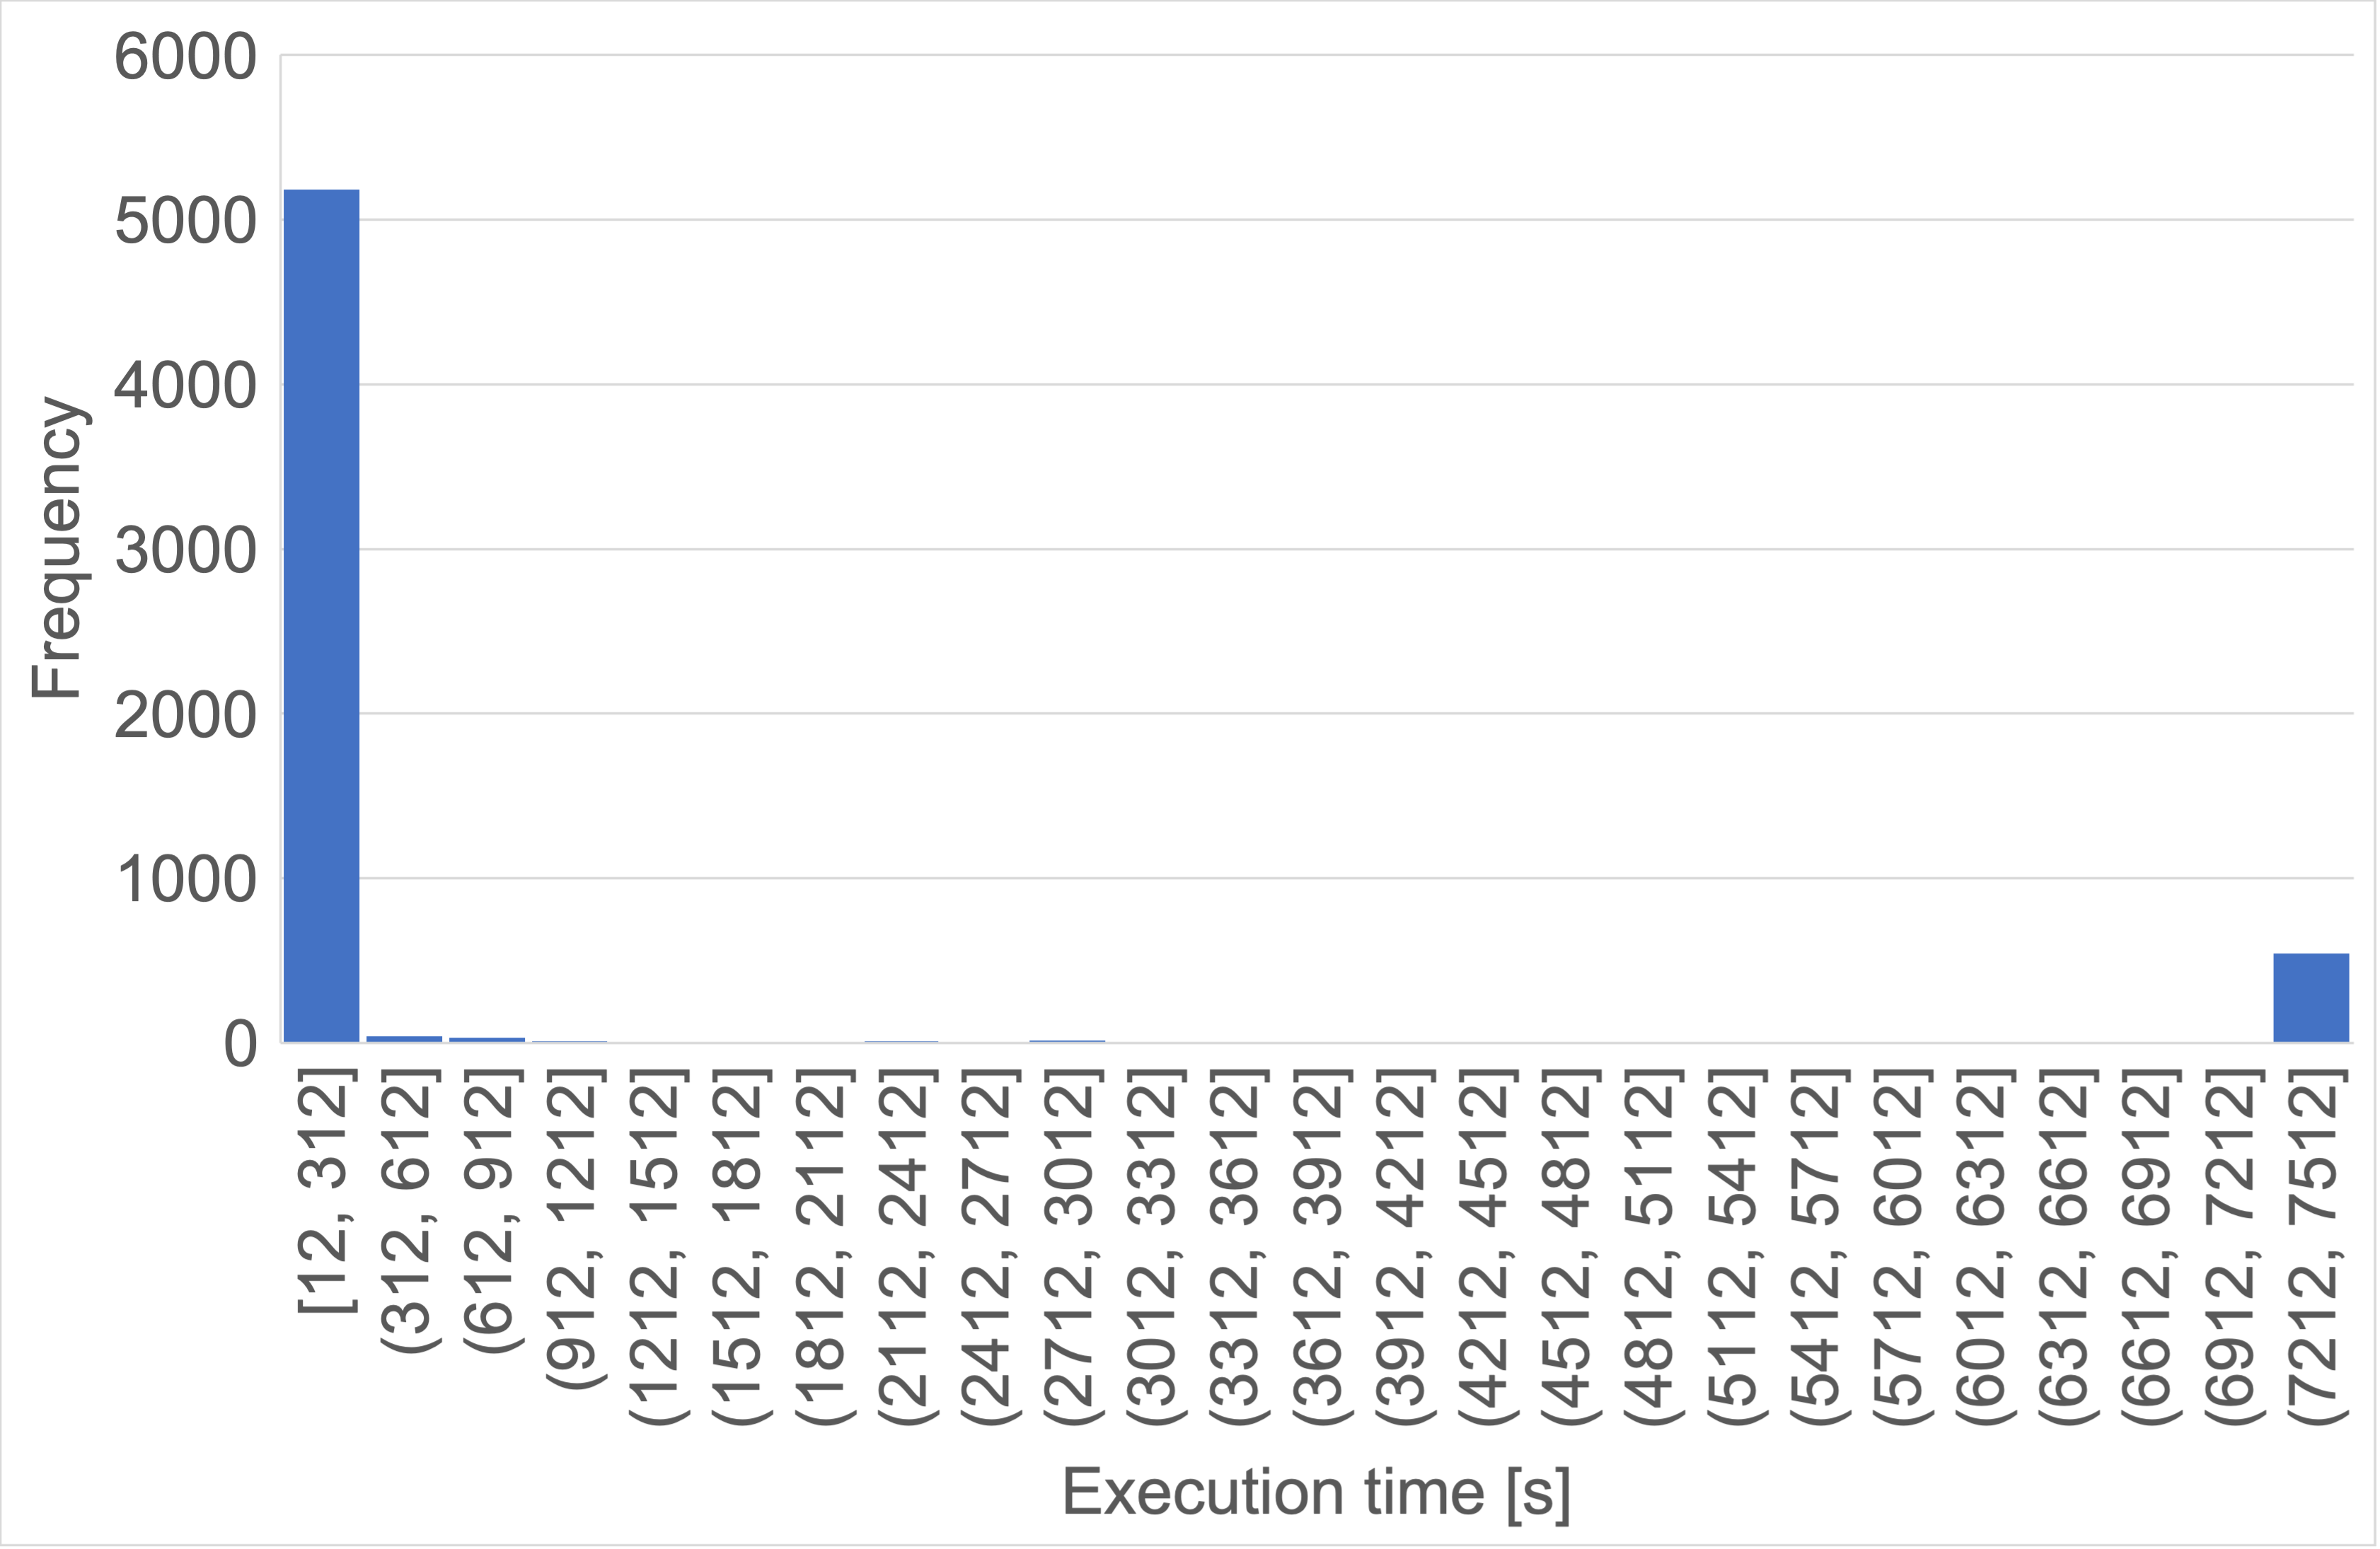
\includegraphics[width=0.7\textwidth]{images/execution_time}
        \caption{SEMuS execution time histogram.}
        \label{fig:semus:histogram_time}
    \end{figure}

\REVOCT{TDR-SUM-PABG-01}{Furthermore, we report in Figure~\ref{fig:semus:histogram_time} the histogram of the execution time of all test cases generated for both ASN.1 and MLFS. Particularly, we can see that for 5\,068 mutants (89.11\%) the test case generation time was approximately 5 minutes, and that only 545 mutants took 2 hours approximately (the maximum time configured for our experiments, which leads to test cases not being generated). In line with these results, we conclude that test generation with SEMuS scale.}


\begin{table}[htb]
\caption{SEMuS execution times.}
\label{table:results:semus:times} 
\centering
\footnotesize
\begin{tabular}{|
@{\hspace{1pt}}p{10mm}|
@{\hspace{1pt}}>{\raggedleft\arraybackslash}p{10mm}@{\hspace{1pt}}|
>{\raggedleft\arraybackslash}p{15mm}@{\hspace{1pt}}|
>{\raggedleft\arraybackslash}p{20mm}@{\hspace{1pt}}|
 >{\raggedleft\arraybackslash}p{15mm}@{\hspace{1pt}}|
 >{\raggedleft\arraybackslash}p{25mm}@{\hspace{1pt}}|
 >{\raggedleft\arraybackslash}p{15mm}@{\hspace{1pt}}|
}
\hline
\textbf{Subject}&\textbf{Min [m]}&\textbf{Max [m]}&\textbf{Median [m]}&\textbf{Mean [m]}&\textbf{Std. Deviation [m]}&\textbf{Total [m]}\\ 
\hline
$\mathit{MLFS}$&0.2&122.5&0.4&8.5&30.2&33\,348.4\\
$\mathit{ASN.1}$&0.2&121.3&0.4&33.4&54.6&69\,696.2\\
\hline
\end{tabular}

\end{table}


\subsection{RQ2 - Approach effectiveness}


To assess the approach effectiveness, we verify whether SEMuS succeeds to generate test inputs that kills non detected mutants from our subjects. We consider SEMuS effective, if the approach improves the subject mutation score.

Table~\ref{table:results:semus:testgen} shows the variations we observed in the subjects' mutation scores, the table presents the number of live mutants, the additionally killed mutants by SEMuS, the original mutation score, and the updated mutation score.
Particularly, we observe that SEMuS kills additional 1\,729 mutants for the ASN.1 subject, increasing the mutation score from 58.31\% to 90.79\%, an impressive improvement of 32,48\%.
Instead, we observe that SEMuS kills additional 697 mutants for the MLFS subject, increasing the mutation score from 81.80\% to 85.06\%, an improvement of 3,26\%.

The lower improvement observed on the MLFS could be explained by the following reasons: (1) possible presence of many equivalent mutants, (2) bugs in SEMuS fixed recently, and (3) known limitations of KLEE (i.e., the underlying test generation tool) concerning floating-point analysis. These limitations can be assessed in a follow up project.

\REVTOOL{C-P-20}{Concering ASN.1CC, SEMuS enabled us to identify a fault in the software; precisely, the ASN.1 test cases did not verify the value of the variable \emph{pErrCode} for functions \emph{\_IsConstraintValid}. The bug was fixed in commit 0917424187be2288c59ac04c804e991aed11a3fe\footnote{{https://github.com/ttsiodras/asn1scc/commit/0917424187be2288c59ac04c804e991aed11a3fe}} ). We also identified another limitation in the test suite; more precisely, the test cases for the function\emph{\_Encode} did not verify that, for the higher-level structure, the return code is zero when the parameter  \emph{bCheckConstraints} is set \emph{false} (basically, an input partition was not covered).}


\REVTOOL{C-P-20}{By definition the quality of the test cases generated by SEMuS shall be high because they kill mutants not killed by the test suite. However, such quality might be diminished by two factors (1) SEMuS erroneously determine that a mutant is killed (this shall be a sort of implementation errors that we never encountered), (2) the mutants are not representative of realistic problems. Concerning (2) we refer the reader to literature indicating that (A) achieving a high mutation score improves significantly the fault detection capability of a test suite~\cite{papadakis2018mutation}, and (B) a very high mutation score (i.e., above 0.75) ensures a higher fault detection rate than the one obtained with other coverage criteria, such as statement and branch coverage~\cite{Chekam:17}.
Based on our observations, we can claim that the generated test cases are of high quality because they (1) cover input partitions not covered by the test suite of the SUT (i.e., the second ASN.1CC case above), (2) enables us to determine  the lack of oracles in the test suite, and (3) enabled the detection of defects (i.e., the ASN.1CC bug reported above).}

For the reasons discussed above, we consider SEMuS an effective solution for test suite improvement in the context of space software.

\begin{table}[htb]
\caption{Subjects' mutation scores after test generation.}
\label{table:results:semus:testgen} 
\centering
\footnotesize
\begin{tabular}{|
@{\hspace{1pt}}p{10mm}|
@{\hspace{1pt}}>{\raggedleft\arraybackslash}p{18mm}@{\hspace{1pt}}|
>{\raggedleft\arraybackslash}p{35mm}@{\hspace{1pt}}|
>{\raggedleft\arraybackslash}p{25mm}@{\hspace{1pt}}|
 >{\raggedleft\arraybackslash}p{25mm}@{\hspace{1pt}}|
}
\hline
\textbf{Subject}&\textbf{Live Mutants}&\textbf{Additionally Killed Mutants}&\textbf{Original MS (\%)}&\textbf{Updated MS (\%)}\\ 
\hline
$\mathit{MLFS}$&3\,891&697&81.80&85.06\\
$\mathit{ASN.1}$&2\,219&1\,729&58.31&90.79\\
\hline
\end{tabular}

\end{table}


\subsubsection{Identifying test suite shortcomings with SEMuS}
\label{sec:shortcoming:semus}

To further analyze SEMuS results, we inspected manually some of the test inputs generated for the ASN.1 case study.
In particular, for the mutant \texttt{test.mut.1298.2\_1\_23.ICR.T\_INT\_IsConstraintValid} we discovered one shortcoming of the ASN.1 test suite. We introduce below detailed information about the mutant under analysis.

The original code of the mutated function, \texttt{T\_INT\_IsConstraintValid}, is shown in Listing~\ref{original_asn_code}.

\begin{lstlisting}[style=CStyle, float=t, caption=Original code., label=original_asn_code]
flag T_INT_IsConstraintValid(const T_INT* pVal, int* pErrCode) {
    flag ret = TRUE;
    (void)pVal;

    ret = ((*(pVal)) <= 50UL);
    *pErrCode = ret ? 0 : ERR_T_INT; 

    return ret;
}
\end{lstlisting}

Listing~\ref{mutant_asn_code} shows the mutated version of the function \texttt{T\_INT\_IsConstraintValid}. Particularly, the mutation operator ICR has replaced the $0$ value on line 6 with a $-1$ value.

\begin{lstlisting}[style=CStyle, float=t, caption=Mutant code., label=mutant_asn_code]
flag T_INT_IsConstraintValid(const T_INT* pVal, int* pErrCode) {
    flag ret = TRUE;
    (void)pVal;

    ret = ((*(pVal)) <= 50UL);
    *pErrCode = ret ? -1 : ERR_T_INT;

    return ret;
}
\end{lstlisting}


Listing~\ref{ktest} shows the KLEE test produced by SEMuS; we observe that SEMuS generated an input for the \texttt{pVal} argument of the function (i.e., an integer of 8 bytes).

\begin{lstlisting}[language={}, float=t, caption=Klee-test output, label=ktest]
ktest file : 'test000001.ktest'
args       : ['/MakeSym-TestGen-Input/direct/T_INT_IsConstraintValid/test.MetaMu.bc']
num objects: 2
object    0: name: b'model_version'
object    0: size: 4
object    0: data: b'\x01\x00\x00\x00'
object    1: name: b'pVal'
object    1: size: 8
object    1: data: b'\x00\x00\x00\x00\x00\x00\x00\x00'
\end{lstlisting}

SEMuS output shows that a \texttt{pVal} value equal to 0 kills the mutant. 
However, we noticed that the ASN.1 test suite already contains test cases with invocations to the \texttt{T\_INT\_IsConstraintValid} function with \texttt{pVal = 0}, in addition to \texttt{pVal = 50}.

Listing~\ref{test_code} shows an excerpt of the ASN.1 test suite, and in particular, the function that verifies the output of \texttt{T\_INT\_IsConstraintValid}. 
We manually verified the reason of \texttt{pVal=0} not being detected by the test suite. Particularly, we notice that after the invocation of the function under test, the value of \texttt{pErrCode} is never checked and it is further re-written on line 10. 

\begin{lstlisting}[style=CStyle, caption=ASN.1 test code., label=test_code]
flag T_INT_enc_dec(const T_INT* pVal, int* pErrCode, const char* filename)
{
    static T_INT decodedPDU;
    flag ret = TRUE;
    ...
            // validate decoded data
            ret = T_INT_IsConstraintValid(&decodedPDU, pErrCode); 
            if (ret) {
                ret = T_INT_Equal(pVal, &decodedPDU);
                *pErrCode = ret ? 0 : 4;
                if (ret) {
                    char buf[1024];
                    strcpy(buf, filename);
                    FILE* fp = fopen(strcat(buf,".dat"), "wb");
                    fwrite(bitStrm.buf, 1, bitStrm.count, fp);
                    fclose(fp);
                }
            }
    ...
}
\end{lstlisting}

We confirmed this shortcoming with ASN.1 engineers, who provided a solution to fix this issue.

% !TEX root = MAIN.tex
\clearpage
\section{Evaluation of Code-driven Mutation Testing Toolsets}
\label{sec:toolsComparison}

This section describes a preliminary evaluation conducted to identify mutation testing tools that are applicable in space context, based on the case study systems of the project. More precisely, for this preliminary evaluation we considered the case study system provided by LuxSpace.

To carry out this preliminary evaluation of mutation testing tools, we selected from the list of mutation testing tools provided in Table 1.1 of deliverable D1, a subset of tools based on the following criteria:

\begin{itemize}
	\item \textbf{Availability of source code.} To enable optimizations, the tool under analysis should be provided along with source code.
	\item \textbf{Applicability to C/C++ code.} The tool under analysis should be able to process C and C++ code.
	\item \textbf{Licence compatible with ESA Software Community Licence Permissive (ESA SCLP).} The licence of the tool under analysis, should enable redistributing the tool itself within the FAQAS framework, which is released under ESA SCLP.
	\item \textbf{Age.} To avoid problems due to support for recent libraries, we should prioritize tools that are recent and actively developed.
\end{itemize}

% !TEX root =  ../MAIN.tex


\setlength\LTleft{0pt}
\setlength\LTright{0pt}
\scriptsize 
\begin{longtable}{@{\extracolsep{\fill}}|p{3.4cm}|p{2.7cm}|p{7cm}|@{}}
\caption{\normalsize Summary of Data-Driven Mutation Testing Benchmarks.}
\label{table:mutationtools} \\
\hline
\textbf{Reference}                   & \textbf{Approach/Tool Name}      & \textbf{Evaluation} \\
\hline
Hariri \& Shi 2018          & SRCIRor                 &
\begin{minipage}[t]{6.5cm}
\textbf{Source code availability.} Yes, https://github.com/TestingResearchIllinois/srciror.\\
\textbf{Applicability to C/C++ code.} Yes.\\
\textbf{ESA SCLP Compatible.} Yes, released under NCSA, https://opensource.org/licenses/NCSA, which allows redistribution and relicensing.\\
\textbf{Age.} Aged, last update in September 2018.\\
\textbf{Outcome. The tool is applicable in space context.} 
\end{minipage}\\
\hline
Wang et al. 2017            & Accmut                  &
\begin{minipage}[t]{6.5cm}
\textbf{Source code availability.} Yes, https://github.com/wangbo15/accmut/\\
\textbf{Applicability to C/C++ code.} Yes.\\
\textbf{ESA SCLP Compatible.} Yes, released under NCSA, https://opensource.org/licenses/NCSA, which allows redistribution and relicensing.\\
\textbf{Age.} Aged, last update in January 2018.\\
\textbf{Outcome. Depends on CLANG/LLVM, which prevents compilations for some sysems.} 
\end{minipage}\\
\hline
Phan et al. 2018            & MUSIC                   &
\begin{minipage}[t]{6.5cm}
\textbf{Source code availability.} Yes, https://github.com/swtv-kaist/MUSIC/\\
\textbf{Applicability to C/C++ code.} Yes.\\
\textbf{ESA SCLP Compatible.} No. The software is licensed with proprietary licence. In private communication via e-mail, authors have shown to be available to relicensing, however this might not fit the budget of the project.\\
\textbf{Age.} Recent, last update in July 2019.\\
\end{minipage}\\
\hline
Denisov \& Pankevich 2018   & Mull                    &
\begin{minipage}[t]{6.5cm}
\textbf{Source code availability.} Yes, https://github.com/mull-project/Mull\\
\textbf{Applicability to C/C++ code.} Yes.\\
\textbf{ESA SCLP Compatible.} Yes. Apache Licence 2.0, https://opensource.org/licenses/Apache-2.0.\\
\textbf{Age.} Ongoing, last update in June 2020.\\
\textbf{Outcome. The tool requires compilation with CLANG/LLVM, which leads to compilation errors with systems depending on RTEMS. Also, natively, Mull performs mutations on the fly through just-in-time compilation features, which is inapplicable if the SUT is executed within a simulator.} 
\end{minipage}\\
\hline
Delgado et al. 2018         & MuCPP                   &
\begin{minipage}[t]{6.5cm}
\textbf{Source code availability.} No, only executables are available https://ucase.uca.es/mucpp/\\
\end{minipage}\\
\hline
Jia \& Harman 2008          & Milu                    &
\begin{minipage}[t]{6.5cm}
\textbf{Source code availability.} Yes, https://github.com/yuejia/Milu/\\
\textbf{Applicability to C/C++ code.} Yes.\\
\textbf{ESA SCLP Compatible.} Yes, released under NCSA licence, https://opensource.org/licenses/NCSA.\\
\textbf{Age.} Aged, last update in April 2018.\\
\textbf{Outcome. The tool generates a preprocessed source code that does not compile.} 
\end{minipage}\\
\hline
Brannstrom et al. 2015      & Dextool                 &
\begin{minipage}[t]{6.5cm}
\textbf{Source code availability.} Yes, https://github.com/joakim- brannstrom/dextool\\
\textbf{Applicability to C/C++ code.} Yes.\\
\textbf{ESA SCLP Compatible.} Yes, released under Mozilla public Licence 2.0, https://opensource.org/licenses/MPL-2.0.\\
\textbf{Age.} Ongoing, last update in June 2020.\\
\textbf{Outcome. Depends on CLANG/LLVM, which prevents compilations for some sysems.} 
\end{minipage}\\
\hline
Delamaro et al. 2001        & Proteum                 &
\begin{minipage}[t]{6.5cm}
\textbf{Source code availability.} Yes, https://github.com/magsilva/proteum.\\
\textbf{Applicability to C/C++ code.} Yes.\\
\textbf{Age.} Aged, last update December 2015.\\
\end{minipage}\\
\hline
Shariar and Zulkernine 2008 & Function Calls Mutation &
\begin{minipage}[t]{6.5cm}
\textbf{Source code availability.} No.\\
\end{minipage}\\
\hline
Dans \& Hierons 2001        & Floating-point Mutation &
\begin{minipage}[t]{6.5cm}
\textbf{Source code availability.} No.\\
\end{minipage}\\  

\hline                                                           
\end{longtable}


\normalsize


The first three criteria mentioned above constitute mandatory requirements. 
Tools not meeting these requirements are not selected for evaluation in our context because they cannot be integrated into the FAQAS framework.
Table~\ref{table:mutationtools} provides the list of tools appearing in Table~1.1 of deliverable D1 along with the evaluation based on the criteria specified above. We do not evaluate all the criteria when one of the mandatory requirements is not met.
For what it concerns the compatibility with the ESA Software Community Licence Permissive, we consider the licenses NCSA and Apache Licence 2.0 compatible. 
Indeed, both the two licences allow for redistribution of the software, a condition that is sufficient to release a mutation testing tool as component of the FAQAS framework.

For our preliminary evaluation we selected the five most recent tools that fulfill our mandatory requirements: SRCIRor, Mull, Dextool, Accmut, and Milu. Proteum has been discarded because its latest stable version dates back to December 2015; on May 2020 a few changes had been made on Proteum GitHub repository, however, the up to date version is indicated by its developer as not usable.

Section~\ref{subsec:experiment_design} provides an overview of the experiment design and the case study considered. 
Section~\ref{subsec:background} provides a brief introduction to the static analysis framework used by all the tools assessed in our study.
Section~\ref{subsec:srciror} to Section~\ref{subsec:dextool} describe the results achieved for each mutation testing tool considered in our study.

As detailed in the following Sections, the only mutation testing tool that is applicable to space software is SRCIRor.

\subsection{Experiment Design and Case Studies}
\label{subsec:experiment_design}




To evaluate the applicability of existing mutation testing tools to space software, we evaluated each mutation testing tool considered in our study against the same case study system of the project, i.e., the System Test Suite for ESAIL provided by LXS. We selected this case study system, because, based on inspection of its specification documents and source code, appears to be the most complicate to process by mutation testing tools. This is mostly due to three criticalities:

\begin{itemize}
	\item ESAIL is the largest case study system of FAQAS in terms of lines of code;
	\item the ESAIL system test suite requires that the full software is compiled and all the required libraries linked (this may complicate the use of tools that cannot parse all the source code);
	\item the software under test (SUT) is executed within a system emulator (SVF) that requires the SUT to respect its real-time constraints.
\end{itemize}

In the following, we provide an overview of ESAIL and the ESAIL System Test Suite. ESAIL consists of 924 source files (719 files with extension ``.c'' and 205 with extension ``.h''). In total, it consists of 74,161 LOC. ESAIL is compiled with sparc-rtems4.8-gcc, a tailored version of the gcc compiler for sparc systems, the compiler is provided by Cobham Gaisler\footnote{https://www.gaisler.com/index.php/products/operating-systems/rtems}.

\begin{figure}[h]
	\centering
    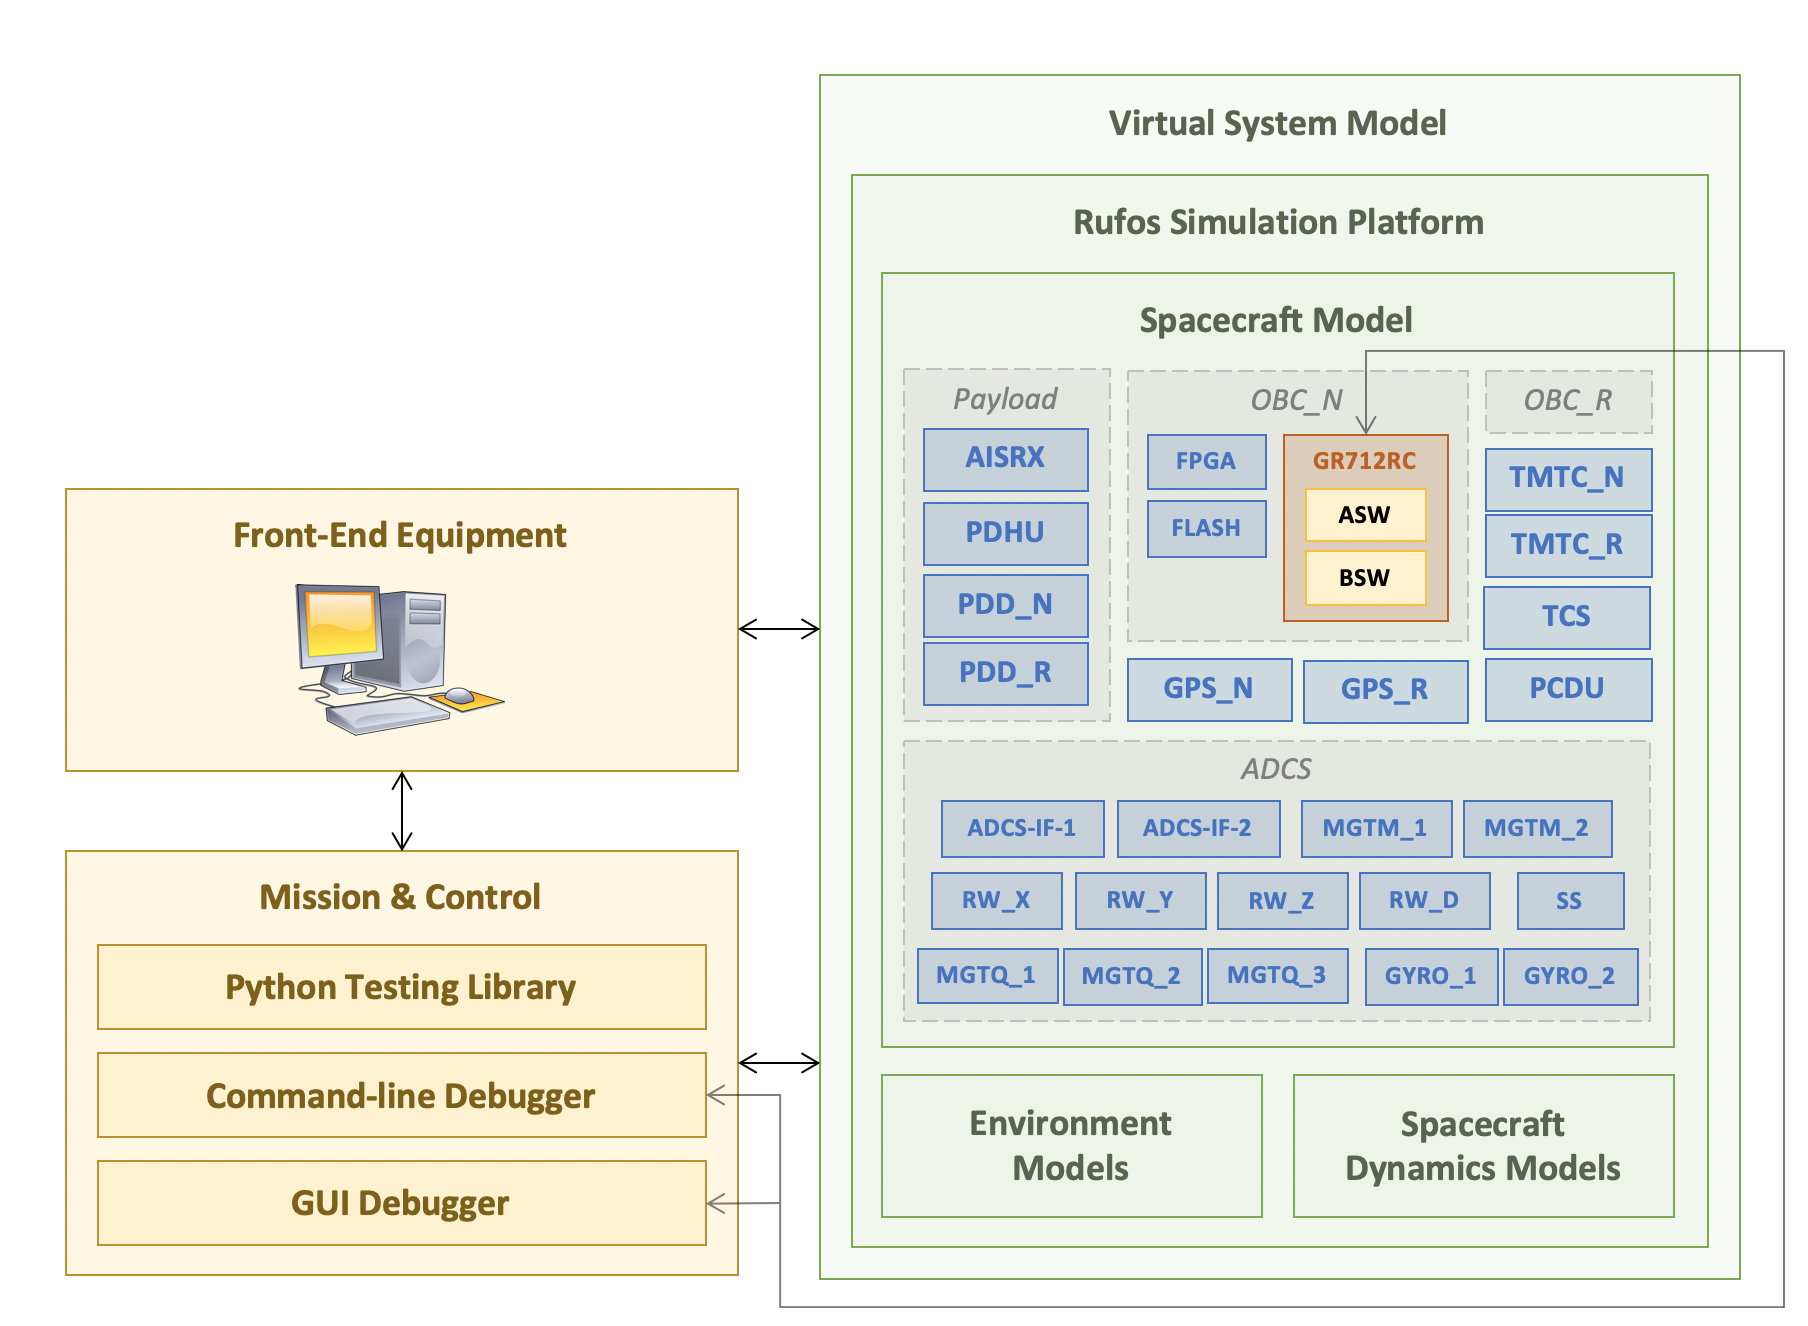
\includegraphics[width=0.7\textwidth]{images/esail}
    \caption{ESAIL system testing environment.}
    \label{fig:esail}
\end{figure}

The architecture of the ESAIL System Testing environment is shown in Figure \ref{fig:esail}. The python testing library is used to execute system test cases that send commands to ESAIL. ESAIL is executed in a simulator based on Rufos. The ESAIL system test suite consists of 121 python programs and it executes in 10 hours, depending on the running environment.

The objective of this preliminary evaluation is to determine if the mutation testing tools considered in our study can process the case study system and automatically generate mutated versions of the case study system that can be successfully compiled and tested. More precisely, we aim to verify if the mutation testing tools considered in our study can successfully create mutated version of ESAIL that can be compiled and executed within the SVF.

\subsection{Background on Clang/LLVM}
\label{subsec:background}

In this section we provide background information on the components that are used by most of the tools considered in our evaluation, i.e., Clang/LLVM.


\begin{figure}[h]
	\centering
    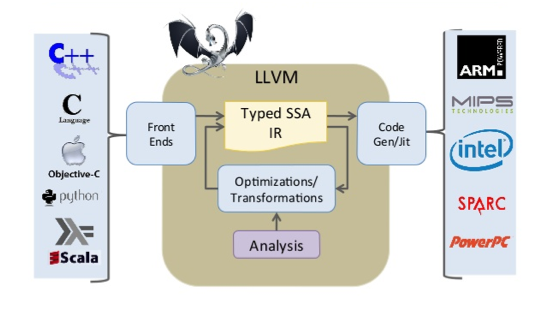
\includegraphics[width=0.5\textwidth]{images/llvm}
    \caption{LLVM compiler infrastructure.}
    \label{fig:llvm}
\end{figure}

The LLVM project is a set of compiler and toolchain technologies. LLVM is designed around an intermediate representation (i.e., LLVM IR) that serves as a portable, high-level assembly language useful for code optimizations. LLVM was originally implemented for C and C++, but now currently it also supports Ada, D, Delphi, Fortran, Haskell, Julia, Objective-C, Rust and Swift. It can be used for performing static analysis on code (e.g., uninitialized memory uses), optimization or code parsing.

Clang is a front-end for LLVM that processes C-family languages: C, C++, Objective C, Objective C++. Clang converts C/C++ to LLVM IR, LLVM performs optimizations on the IR, and the LLVM x86 backend writes out x86 machine code for execution.

\subsection{Evaluation of SRCIRor}
\label{subsec:srciror}

\subsubsection{Overview of the mutation testing tool}

SRCIRor is LLVM-based mutation testing tool that works at the level of source code (SRC), and the LLVM compiler intermediate representation (IR). 
At a source code level SRCIRor performs mutations by using the clang compiler to parse the input files and build the abstract syntax trees (AST). 
At the IR level SRCIRor finds and directly mutates the instructions of interest, which might be all the instructions of the SUT or a subset of them. 
SRCIRor implements six types of operators, it implements Arithmetic Operators (e.g., $+, -, *, /, \%$), Relational Operators (e.g., $<, <=, >, >=, ==, !=$), Logical Operators (e.g., $\&\&, ||$), Bitwise Operators (e.g., $\&, |, \wedge$), Arithmetic Assignment Operators (e.g., $+=, -=, *=, /=, \%=$) and Bitwise Assignment Operators (e.g., $\&=, |=, \wedge=$).

\begin{figure}[h]
	\centering
    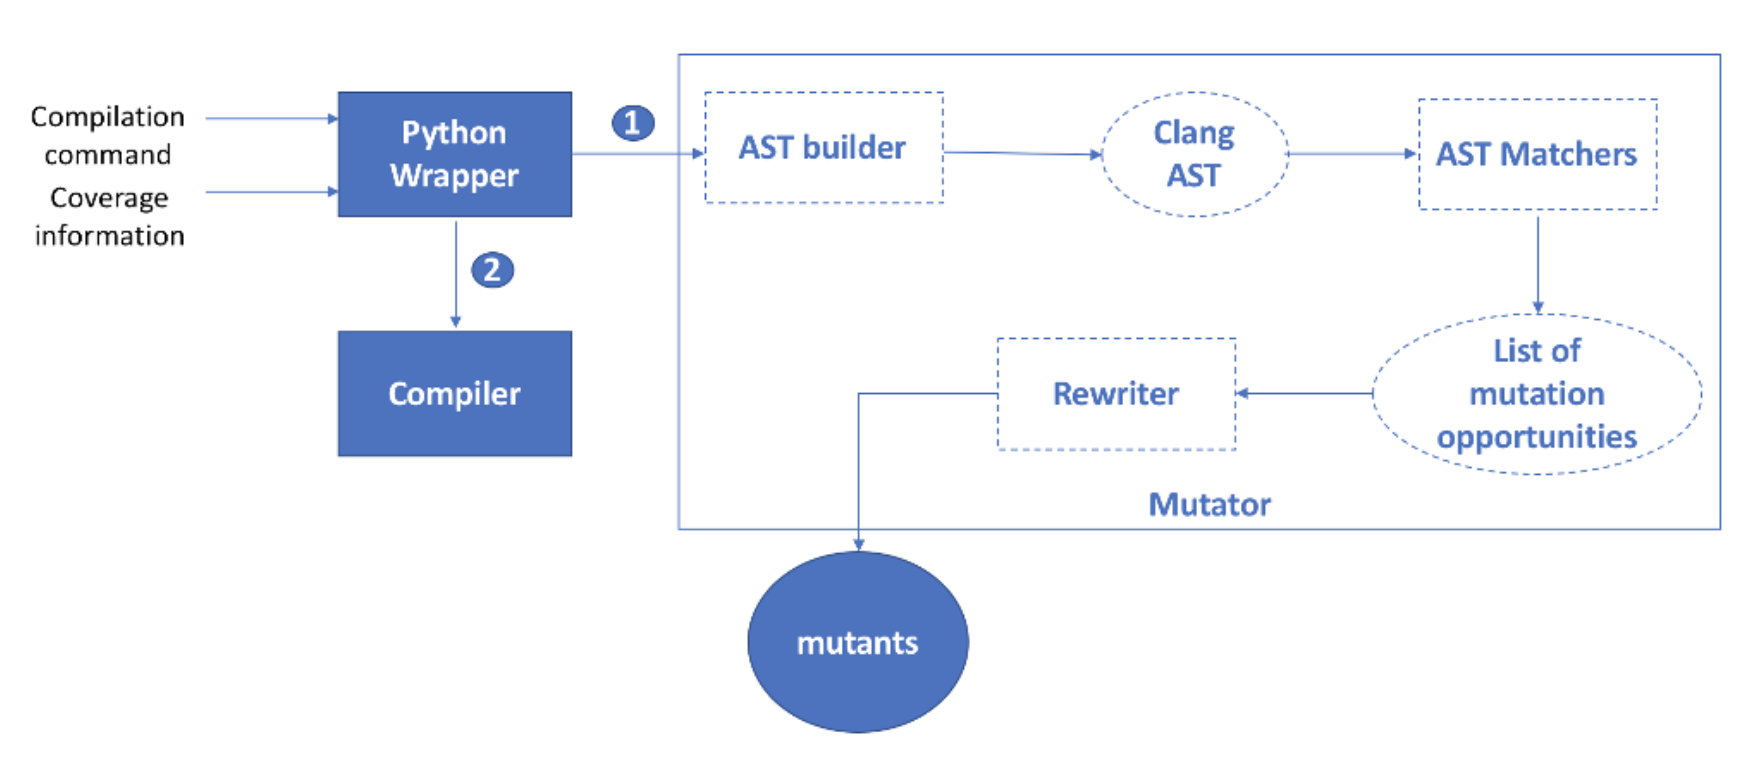
\includegraphics[width=0.75\textwidth]{images/srciror_arch}
    \caption{SRCIRor architecture. Source Hariri et al.~\cite{hariri2018srciror}.}
    \label{fig:srciror_arch}
\end{figure}

\MREVISION{C-P-23}{Figure~\ref{fig:srciror_arch} shows the architecture of SRCIRor. The mutations are done in three steps: in (1) the clang parser with the help of a Python wrapper, processes the input files and builds the abstract syntax tree (AST). Then, in (2), SRCIRor implements ASTMatchers to identify the mutation points along the AST. ASTMatchers are a domain specific language for querying the AST in a simple manner, for example, to implement the ICR mutation operator is enough to make a call to the ASTMatcher \texttt{integerLiteral()} to obtain all the integer literals present in the AST. Finally, in (3), SRCIRor uses again clang to perform the source to source transformation by directly modifying the source code, the transformation is then applied iteratively for all the mutation points identified in (2).}

\subsubsection{Results}

%The main objective of FAQAS of this project is being able to apply mutation testing techniques to space software. To assess the compatibility of SRCIRor with FAQAS we applied the tool to one of our case studies, in this case, we selected the ESAIL SVF software.
The mutation process has been executed by applying the SRCIRor source code mutator to every .c file in the ESAIL SVF project. We applied the default configuration of SRCIRor, that is, applying the six operators and mutating every line within the source code files.
From the results, we observe the generation of 105\,543 mutants. However, during the pass of SRCIRor we detected 1\,060 warnings thrown by the clang input parser.

Most of the warnings are caused by SRCIRor trying to mutate memory addresses declared in C code, (e.g., mutating \texttt{0x03A6} into \texttt{(- 1)x03A6}), and unsigned integer literals (e.g., \texttt{0u}, \texttt{1u} into \texttt{(-1)u}, \texttt{1u}).
Listing~\ref{srciror_1} to Listing~\ref{srciror_10} list the representative cases for all the warning classes found during the mutation process. 

Listing~\ref{srciror_1} shows a warning due to an incompatibility with duplicate keywords declaration. 
Listing~\ref{srciror_2} shows a warning related to the magnitude of a floating-point variable. 
Listing~\ref{srciror_3} shows a warning due to an implicit conversion from an enumeration type. 
Listing~\ref{srciror_4} shows a warning related to an uninitialized variable being used. 
Listing~\ref{srciror_5} shows a warning due to a variable not being used in the source code. 
Listing~\ref{srciror_6} shows a warning related to an invalid cast. 
Listing~\ref{srciror_7} shows a warning related to a clang problem with inline functions. 
Listing~\ref{srciror_8} shows multiple warnings on inline functions and invalid casts.
Listing~\ref{srciror_9} shows a warning due to an inappropriate use of parentheses. Finally, Listing~\ref{srciror_10} shows a warning related to incompatible declarations of already existing library functions. 

% !TEX root = ../MAIN.tex

\noindent\begin{minipage}{\textwidth}
\begin{lstlisting}[language={}, caption=1st warning example., label=srciror_1]
In file included from /home/svf/Obsw/Source/ApplicationLayer/SYS_KeepAlive/Source/SoftKeepAliveTask.c:50: 
././HighLevelDriverLayer/EPS_Handler/Public/epshdl_Api.h:125:104: 
warning: duplicate 'const' declaration specifier [-Wduplicate-decl-specifier]
epshdlr_status_code_t epshdl_MemoryWrite(const uint16_t memAddr, const uint16_t memLen, const uint16_t const *memDataPtr);
													  ^
1 warning generated.
\end{lstlisting}
\end{minipage}
% !TEX root = ../MAIN.tex

\noindent\begin{minipage}{\textwidth}
\begin{lstlisting}[language={}, caption=2nd warning example., label=srciror_2]
/home/svf/Obsw/Source/ApplicationLayer/AdcsController/Source/strtod.c:122:12: warning: magnitude of floating-point constant too large for type 'double'; maximum is 1.7976931348623157E+308 [-Wliteral-range]
return HUGE_VAL; 
			 ^
./_Ext/mlfs/include/mlfs.h:147:19: note: expanded from macro 'HUGE_VAL' #define HUGE_VAL (1.0e999999999)
							^ 
1 warning generated.
\end{lstlisting}
\end{minipage}
% !TEX root = ../MAIN.tex

\noindent\begin{minipage}{\textwidth}
\begin{lstlisting}[language={}, caption=3rd warning example., label=srciror_3]
/home/svf/Obsw/Source/ApplicationLayer/AdcsController/Source/adcs_DetermineSatellitePosition.c: 222:41: warning: implicit conversion from enumeration type 'cast_Status_t' (aka 'enum cast_Status_e') to different enumeration type 'prep_ResponseCode_t' (aka 'enumprep_ResponseCode_e') 
[-Wenum-conversion]
adem_SetDeterminedSatellitePosition(Status,*SatState_Ptr,OnBoardTime);
~~~~~~~~~~~~~~~~~~~~~~~~~~~~~~~~~~~ ^~~~~~ 
1 warning generated
\end{lstlisting}
\end{minipage}
% !TEX root = ../MAIN.tex

\noindent\begin{minipage}{\textwidth}
\begin{lstlisting}[language={}, caption=4th warning example., label=srciror_4]
In file included from /home/svf/Obsw/Source/ApplicationLayer/PDHU_Handler/Source/PDHU_handler.c:40:
In file included from ././ApplicationLayer/PDHU_Handler/Private/PDHU_handler.h:31:
In file included from ././ApplicationLayer/PDHU_Handler/Public/PDHU_handler_Api.h:34: ././HighLevelDriverLayer/EPS_Handler/Public/epshdl_Api.h:125:104: warning: duplicate 'const' declaration specifier [-Wduplicate-decl-specifier]
epshdlr_status_code_t epshdl_MemoryWrite(const uint16_t memAddr, const uint16_t memLen, const uint16_t const *memDataPtr);
														^
/home/svf/Obsw/Source/ApplicationLayer/PDHU_Handler/Source/PDHU_handler.c:1302:8: warning: variable 'received_size' is used uninitialized whenever 'if' condition is false [-Wsometimes- uninitialized]
	if(is_PDHU_on() == true) 
			^~~~~~~~~~~~~~~~~~~~
/home/svf/Obsw/Source/ApplicationLayer/PDHU_Handler/Source/PDHU_handler.c:1316:8: note: uninitialized use occurs here
	if(received_size != PDHU_EVENT_LOG_SIZE) 
			^~~~~~~~~~~~~
/home/svf/Obsw/Source/ApplicationLayer/PDHU_Handler/Source/PDHU_handler.c:1302:5: note: remove the 'if' if its condition is always true
	if(is_PDHU_on() == true)
			^~~~~~~~~~~~~~~~~~~~~~~~ 
/home/svf/Obsw/Source/ApplicationLayer/PDHU_Handler/Source/PDHU_handler.c:1300:27: note: initialize the variable 'received_size' to silence this warning
	uint32_t received_size; 
											  ^
										  	= 0
2 warnings generated.
\end{lstlisting}
\end{minipage}
% !TEX root = ../MAIN.tex

\noindent\begin{minipage}{\textwidth}
\begin{lstlisting}[language={}, caption=5th warning example., label=srciror_5]
/home/svf/Obsw/Source/ApplicationLayer/AdcsDataExchangeManager/Source/adem_GetReactionwheelMeas InEng.c:44:21: warning: unused variable 'RW_ACCELERATION_COEFF' [-Wunused-const-variable]
static const double RW_ACCELERATION_COEFF 	= 3.75e-3;
/* RW_ACCELERATION_COEFF 0.00375 rpm/s per digit as per ICD RW 90

1 warning generated.
\end{lstlisting}
\end{minipage}
% !TEX root = ../MAIN.tex

\noindent\begin{minipage}{\textwidth}
\begin{lstlisting}[language={}, caption=6th warning example., label=srciror_6]
/home/svf/Obsw/Source/HighLevelDriverLayer/OBC_Handler/Source/ObcHandler_ProcessingTask.c:130:3 6: warning: cast to 'uint8_t *' (aka 'unsigned char *') from smaller integer type 'unsigned int' [-Wint-to-pointer-cast]
	CurrentSampleAddress_ptr = (uint8_t*)(EEPROM_START_ADDRESS + PATTERN_OFFSET + PatternCheck[SampleIndex].Offset);
															^
1 warning generated.
\end{lstlisting}
\end{minipage}
% !TEX root = ../MAIN.tex

\noindent\begin{minipage}{\textwidth}
\begin{lstlisting}[language={}, caption=7th warning example., label=srciror_7]
In file included from /home/svf/Obsw/Source/LowLevelDriverLayer/apbuart/Source/drv_uart.c:47: ././LowLevelDriverLayer/core/Public/coreApi.h:193:12: warning: inline function 'loadmem' is not defined [-Wundefined-inline]
inline int loadmem(int addr); /home/svf/Obsw/Source/LowLevelDriverLayer/apbuart/Source/drv_uart.c:553:18: note: used here
	reg_status = loadmem((int)&uart->regs->status);
In file included from /home/svf/Obsw/Source/LowLevelDriverLayer/apbuart/Source/drv_uart.c:61: ././LowLevelDriverLayer/apbuart/Private/drv_uartFifo.h:100:20: warning: inline function 'ff_FifoIsEmpty' is not defined [-Wundefined-inline]
extern inline bool ff_FifoIsEmpty(uint32_t const Fifo_ID); /home/svf/Obsw/Source/LowLevelDriverLayer/apbuart/Source/drv_uart.c:653:13: note: used here
	if (ff_FifoIsEmpty(uart->txfifoId) == true)
In file included from /home/svf/Obsw/Source/LowLevelDriverLayer/apbuart/Source/drv_uart.c:61: ././LowLevelDriverLayer/apbuart/Private/drv_uartFifo.h:108:24: warning: inline function 'ff_FifoBytesWaiting' is not defined [-Wundefined-inline]
extern inline uint32_t ff_FifoBytesWaiting(uint32_t const Fifo_ID); /home/svf/Obsw/Source/LowLevelDriverLayer/apbuart/Source/drv_uart.c:1047:30: note: used here
	NbBytesWaiting = ff_FifoBytesWaiting(uart->rxfifoId); 

3 warnings generated.
\end{lstlisting}
\end{minipage}
% !TEX root = ../MAIN.tex

\noindent\begin{minipage}{\textwidth}
\begin{lstlisting}[language={}, caption=8th warning example., label=srciror_8]
/home/svf/Obsw/Source/LowLevelDriverLayer/GRTC/Source/drv_GRTC.c:235:15: warning: cast to 'unsigned short *' from smaller integer type 'unsigned int' [-Wint-to-pointer-cast]
	if ((*(unsigned short *)(rp)&0x00ff) == 0x01) 
				 ^
/home/svf/Obsw/Source/LowLevelDriverLayer/GRTC/Source/drv_GRTC.c:244:36: warning: cast to 'unsigned short *' from smaller integer type 'unsigned int' [-Wint-to-pointer-cast]
	cnt = grtcprv_scan((unsigned short *)(rp), upper, 0x01, &found); 
											^			
/home/svf/Obsw/Source/LowLevelDriverLayer/GRTC/Source/drv_GRTC.c:396:46: warning: cast to 'unsigned short *' from smaller integer type 'int' [-Wint-to-pointer-cast]
	if (grtcprv_check_ending((unsigned short *)(rp), cnt - 2, 1)) 
														^
/home/svf/Obsw/Source/LowLevelDriverLayer/GRTC/Source/drv_GRTC.c:404:46: warning: cast to 'unsigned short *' from smaller integer type 'int' [-Wint-to-pointer-cast]
	if (grtcprv_check_ending((unsigned short *)(rp), cnt, 0)) 
														^
/home/svf/Obsw/Source/LowLevelDriverLayer/GRTC/Source/drv_GRTC.c:514:41: warning: 'unsigned short *' from smaller integer type 'unsigned int' [-Wint-to-pointer-cast]
	if ((tot = grtcprv_copy((unsigned short *)(rp), buf, cnt)) != cnt) 
													 ^
In file included from /home/svf/Obsw/Source/LowLevelDriverLayer/GRTC/Source/drv_GRTC.c:50: ././LowLevelDriverLayer/core/Public/coreApi.h:193:12: warning: inline function 'loadmem' is not defined [-Wundefined-inline]
	inline int loadmem(int addr);
							^
/home/svf/Obsw/Source/LowLevelDriverLayer/GRTC/Source/drv_GRTC.c:203:10: note: used here
	rp = loadmem((int)&grtcDev.regs->rrp); 
			 ^

6 warnings generated.
\end{lstlisting}
\end{minipage}
% !TEX root = ../MAIN.tex

\noindent\begin{minipage}{\textwidth}
\begin{lstlisting}[language={}, caption=9th warning example., label=srciror_9]
/home/svf/Obsw/Source/ServiceLayer/Data_Store/Source/Store_TM.c:995:35: warning: equality comparison with extraneous parentheses [-Wparentheses-equality]
	if((Storage_Ptr->tail == Storage_Ptr->header)) 
			~~~~~~~~~~~~~~~~~~^~~~~~~~~~~~~~~~~~~~~~
/home/svf/Obsw/Source/ServiceLayer/Data_Store/Source/Store_TM.c:995:35: note: remove extraneous parentheses around the comparison to silence this warning
	if((Storage_Ptr->tail == Storage_Ptr->header)) 
			~									^			~
/home/svf/Obsw/Source/ServiceLayer/Data_Store/Source/Store_TM.c:995:35: note: use '=' to turn this equality comparison into an assignment
	if((Storage_Ptr->tail == Storage_Ptr->header)) 
												^~
						  					=
1 warning generated.
\end{lstlisting}
\end{minipage}
% !TEX root = ../MAIN.tex

\noindent\begin{minipage}{\textwidth}
\begin{lstlisting}[language={}, caption=10th warning example., label=srciror_10]
In file included from /home/svf/Obsw/Source/Utilities/Misc/Source/mini_rtl.c:31: ././Utilities/Misc/Public/mini_rtl.h:14:10: warning: incompatible redeclaration of library function 'strlen' [-Wincompatible-library-redeclaration]
	unsigned strlen(const char *q);
					  ^
././Utilities/Misc/Public/mini_rtl.h:14:10: note: 'strlen' is a builtin with type 'unsigned long (constchar *)'
././Utilities/Misc/Public/mini_rtl.h:17:5: warning: incompatible redeclaration of library function 'memcmp' [-Wincompatible-library-redeclaration]
	int memcmp(const char *s1, const char *s2, size_t n);
			^
././Utilities/Misc/Public/mini_rtl.h:17:5: note: 'memcmp' is a builtin with type 'int (const void *, const void *, unsigned long)'

2 warnings generated.
\end{lstlisting}
\end{minipage}

To evaluate if the generated mutants can be successfully compiled, we executed the ESAIL compilation process for all the generated 105\,543 mutants. From the total, 103\,747 mutants (98.3\%) were compiled successfully using the original ESAIL settings.

\subsection{Evaluation of Mull}
\label{subsec:mull}

\subsubsection{Overview of the mutation testing tool}

Mull is an open source tool for mutation testing of C/C++ software based on the LLVM framework. Mull works at the intermediate representation level, i.e., the mutations are applied on the instructions residing in the LLVM bitcode files. It relies on debug information to show results, for this reason it requires that the SUT is compiled with clang and the \texttt{-fembed-bitcode} and debug information enabled. \MREVISION{C-P-25}{Mull does not work at source code level.}

The mutation process in Mull consists of the following steps: (1) extracting bitcode files from the executable artifact, (2) finding test cases related to the executable by running the test suite, (3) searching/filtering for mutation points, based on the coverage of the test suite execution, (4) compiling the possible mutations, (5) inserting memory trampolines on the original functions, then compile only the part of bitcode that had been mutated, and (6) running the test cases that cover the mutated function.

Mull generates mutants on the fly, while the SUT is executed against the test suite. To this end it relies on the JIT feature of LLVM. This feature enables the compilation of code on the fly as it is needed, with no necessity of re-compiling the whole program on disk. The online nature of Mull enables it to implement a set of optimizations that speed up the mutation process. A list of optimizations follows.

\begin{itemize}
	\item Dynamic Call Tree: optimization for mutating source code reachable by the test cases
	\item LLVM JIT engine: compilation and linking of the new mutants happen in memory, thus there is no disk I/O overhead.
	\item Sandboxing: run each test in a separate child process, this way, if the child process fails it will not affect the parent process.
	\item Dry-run: collect information in advance about how many mutations a project has and how much time does it take to run it.
	\item Caching: save mutants on disk; for future executions Mull tries first loading the object file from the cache first.
	\item Fail-fast mode: once a mutant is killed by a test case it is no longer executed against other test cases.
\end{itemize}

Although the optimization features of Mull reduce the overall execution time of the mutation process, the online nature of Mull prevents its application to ESAIL. Indeed, ESAIL runs within an emulated environment that requires an executable compiled for the actual platform of the system. This prevents the execution of the JIT feature of the LLVM infrastructure. In the following paragraphs, we provide an overview of the modifications we implemented on Mull to apply it to our case study.

\subsubsection{Extending Mull's features}

%To evaluate Mull, we mutated one of the example projects provided by the tool authors, the fmt library. The fmt library is an open-source formatting library for C++\footnote{https://github.com/fmtlib/fmt} that can be used as alternative to (s)printf and iostreams.

We adapted Mull to statically generate mutants and save them permanently. Specifically, we developed a module that generates an object file each time a new mutant is identified for a specific module. Then, to generate the final executable, we perform the following actions for each mutated object file: (1) replace the original object file with the mutated one, (2) re-launch the original Makefile (this will generate a new version of the program), and (3) save the executable with a specific identifier (i.e., program name followed by the identifier of the mutant created by Mull).

\subsubsection{Results}

Mull requires compilation with clang. For this reason, we had to replace the original \texttt{rtems-gaisler-gcc} compiler with clang. In particular, we compiled ESAIL with four different compilers:

\begin{enumerate}
	\item RTEMS 4.10 and clang 5 (LLVM version)
	\item RTEMS 5 and gcc (RTEMS version)
	\item RTEMS 5 and clang (RTEMS version)
	\item RTEMS 4.8 and clang 9 (LLVM version)
\end{enumerate}

\begin{enumerate}
	\item \textbf{Compilation with RTEMS 4.10 and clang 5 (LLVM version)}

	To successfully compile the project and address "unsupported target" errors we have modified the following in the RTEMS definition files:

	\begin{itemize}
		\item \texttt{/opt/rtems-4.10/sparc-rtems/include/machine/\_types.h}: commented from line 15 to line 29 (error unsupported target)
	\end{itemize}

	However, we did not succeed in compiling the project because clang does not handle the architectures supported by RTEMS. This is shown by the error:

	% !TEX root = ../MAIN.tex

\noindent\begin{minipage}{\textwidth}
\begin{lstlisting}[language={}]
/opt/rtems-4.10/sparc-rtems/leon3/lib/include/sys/ioccom.h:94:9: error: unknown type name 'u_int32_t' typedef u_int32_t ioctl_command_t;
\end{lstlisting}
\end{minipage}

	\item \textbf{Compilation with RTEMS 5 and clang (RTEMS version)}

	To compile the system, we modified the following in the ESAIL source code:

	\begin{itemize}
		\item \texttt{./ApplicationLayer/SystemInit/Public/systemInit.h}: as shown in the example of the source \texttt{rtems-soft-float.c} we set to false the if condition at the line 99. The problem is that several \texttt{drvmgr.h} constant definitions are no longer available in RTEMS 5.
		
		\item \texttt{./LowLevelDriverLayer/apbuart/Source/drv\_uart.c}: commented the inclusion of the header \texttt{\textless rtems/score/types.h\textgreater}, because it does not exist anymore on RTEMS 5.

		\item \texttt{./ProtocolLayer/CANDispatcher/Source/process\_Heartbeat.c}: the constant \texttt{RTEMS\_CLOCK\_GET\_TICKS\_SINCE\_BOOT} is no longer defined in RTEMS 5, so we made the following change:
		
		\begin{itemize}
			\item Modified this line: \texttt{rtems\_clock\_get(RTEMS\_CLOCK\_GET\_TICKS\_SINCE\_BOOT, \&current\_time);}
			\item By this one:        \texttt{current\_time = rtems\_clock\_get\_ticks\_since\_boot();}
		\end{itemize}
		
		\item \texttt{./Utilities/Misc/Source/cpuLoad.c}: the class \texttt{rtems\_tcb} no longer contains a field called \texttt{real\_priority}, in RTEMS now is \texttt{Real\_priority.priority}, so we applied the change.
	\end{itemize}

	In this case, the ESAIL SVF compiles, but with several warnings, an example is shown in Listing~\ref{rtems5_error}.

	% !TEX root = ../MAIN.tex

\noindent\begin{minipage}{\textwidth}
\begin{lstlisting}[language={}, caption=ESAIL compilation warning with RTEMS 5 and clang., label=rtems5_error]
In file included from ./ApplicationLayer/Operational_Sequences/Source/SpacecraftConfigurationVector.c:36: ./Utilities/./Tools/Public/tool_DataManipulationApi.h:174:9: warning: 'BIT_SET' macro redefined [-Wmacro-redefined]
#define BIT_SET(_InputValue,_BitPos) ((_InputValue) |= (1u << (_BitPos)))
	^
/opt/rcc-1.3-rc6-llvm/bin/../sparc-gaisler-rtems5/include/sys/bitset.h:55:9: note: previous definition is here
#define BIT_SET(_s, n, p) \
	^

1 warning generated.
\end{lstlisting}
\end{minipage}

	Despite successful compilation, the execution did not succeed. When trying to boot up the ESAIL SVF software two errors are thrown that makes impossible the execution of any test case:
	\begin{itemize}
		\item Sender: OBC/OBC1/FPGA, message: Watchdog reset \texttt{[0x00000000]}.
		\item Sender: Python, message: message: No OBC powered.
	\end{itemize}

	\item \textbf{Compilation with RTEMS 5 and gcc (RTEMS version)}

	We switched to gcc instead of clang, to determine if the problems were due to the clang or RTEMS version. For this case, we applied the same changes done for case 2.
	Despite the changes above lead to successful compilation of the object code, they did not solve all the compilation problems. Indeed, an ESAIL executable cannot be created because of linking error, the linker claims several undefined references such as:

	% !TEX root = ../MAIN.tex

\noindent\begin{minipage}{\textwidth}
\begin{lstlisting}[language={}]
ld: warning: cannot find entry symbol start; defaulting to 40000000

/opt/rcc-1.3-rc6-gcc/sparc-gaisler-rtems5/leon3/lib/librtemsbsp.a(bspgetworkarea.o): In function `bsp_work_area_initialize’:
/opt/rcc-1.3-rc6-gcc/src/rcc-1.3- rc6/c/src/lib/libbsp/sparc/leon3/../../../../../../bsps/sparc/shared/start/bspgetworkarea.c:32: undefined reference to `rdb_start'
\end{lstlisting}
\end{minipage}

	\item \textbf{Compilation with RTEMS 4.8 and clang 9 (LLVM version)}
	
	In the fourth attempt of ESAIL compilation, we tried to build the software with the token \texttt{release=true} as suggested by LuxSpace. Even though, clang is now able to handle RTEMS libraries, still we get an error that does not allow successful ESAIL compilation:

	% !TEX root = ../MAIN.tex

\noindent\begin{minipage}{\textwidth}
\begin{lstlisting}[language={}]
error: unexpected token in argument list
__asm__ volatile (" lda [%1]1, %0\n" : "=r"(tmp) : "r"(addr));
	^
<inline asm>:1:13: note: instantiated into assembly here lda [%eax]1, %eax
\end{lstlisting}
\end{minipage}

	From Leon documentation, the number after the brackets means a specific Address Space Identifier (ASI), where in this case 1 means forced cache miss. Applied to the specific, clang does not recognize the 1 after the '[\%1]' token.

\end{enumerate}

\MREVISION{C-P-25}{Even though, Mull implement several runtime optimizations, unfortunately for the scope of this project is not possible to consider it, since it forces the use of a specific compiler (i.e., the clang compiler). Therefore, a mutation testing tool that relies on a specific compiler reduces the chances of applying the technique on the context of space software. For example, ESAIL relies on the Sparc RTEMS compiler, so it would out of the scope if we rely on the Mull toolset.}

\subsection{Milu Evaluation Results}
\label{subsec:milu}

\subsubsection{Overview of the mutation testing tool}

Milu is an efficient and flexible C mutation testing tool designed for both first order and higher order mutation testing. Milu is a LLVM-based tool that works at source-code (SRC) level. It performs mutations by using the clang compiler to parse the input files and build the Abstract Syntax Tree (AST) representation of the source code.

The tool implements the following first-order operators:
\begin{itemize}
	\item Absolute Value Insertion (ABS)
	\item Arithmetic Operator Replacement (AOR)
	\item Logical Connector Replacement (LCR)
	\item Relational Operator Replacement (ROR)
	\item Unary Operator Insertion (UOI)
	\item Integer Constant Replacement (CRCR)
	\item Arithmetic Assignment Mutation (OAAA)
	\item Logical Context Negation (OBBN)
	\item Statement Deletion (SSDL)
\end{itemize}

In addition, it also implements the following memory mutation operators:
\begin{itemize}
	\item Replace calloc with malloc (REC2M)
	\item Remove null character assignment statement (RMNA)
	\item Replace calls malloc, calloc, alloca and realloc with null (REDAWN)
	\item Replace size of the requested block with 0 for dynamic memory allocation functions
	(REDAWZ)
	\item Replace the arguments of the sizeof unary operator with the pointer type equivalent if a
	non-pointer type is specified (RESOTPE)
	\item Replace the arguments of the sizeof unary operator with the non-pointer type equivalent
	if a pointer type is specified (REMSOTP)
	\item Remove free statement (RMFS)
	\item Replace malloc with alloca (REM2A)
	\item Replace calloc with alloca (REC2A) 
\end{itemize}


\subsubsection{Results}

Despite Milu has been highly referenced in the literature, it is, nowadays, an outdated tool that is no longer supported by authors.
To generate mutants with Milu it is necessary to pre-process the source files of the system under test with \texttt{gcc -E}, this option will expand all the macros contained in a single source code file.

In our evaluation, the mutation process has been performed by applying the Milu source code mutator to the \texttt{adcs\_ExecuteReactionwheelDesaturation} source file of the \texttt{ApplicationLayer} component, for this example we selected the \linebreak\texttt{adcs\_ExecuteReactionwheelDesaturation} function to be mutated. We applied the default configuration of Milu, that is, applying all the first-order operators to every line in the function under analysis.

However, the mutation process of this source file leads to a segmentation fault in the line \texttt{if(g\_strcmp0(func\_name, tmp\_node -> text) == 0)} of the \linebreak\texttt{milu\_project\_load\_function\_settings} function in Project.c. In particular, when debugging the mutation process with \texttt{gdb}, we observe that there is a variable called \texttt{tmp\_node->text} that contains corrupted data:

\noindent\begin{minipage}{0.8\textwidth}
\begin{lstlisting}[language={}]
$1 = (gchar *) 0xe <Address 0xe out of bounds>
\end{lstlisting}
\end{minipage}

Through a manual inspection of the Milu source code, we found that there are two functions aimed to clean the abstract syntax tree (e.g., fix\_function\_attribute and clean\_ast) that are introducing corrupted data into the AST data structure processed by Milu.
By commenting out these two functions, it was possible to execute the mutation process of the adcs\_ExecuteReactionwheelDesaturation source file. 

Milu produces 35 mutants belonging to the adcs\_ExecuteReactionwheelDesaturation function.
\EMPH{However, it is not possible to compile any of the 35 mutants produced by Milu.} We observe errors during the ESAIL compilation process, in particular there are errors being thrown from the preprocessed area of the mutant. In Listing~\ref{miluerror}, an example of the error obtained during compilation is shown.

\noindent\begin{minipage}{\textwidth}
\begin{lstlisting}[language={}, caption=Error obtained during mutant compilation process in ESAIL., label=miluerror]
In file included from ././ApplicationLayer/AdcsController/Public/Adcs_Api.h:47,
				 from ./ApplicationLayer/AdcsController/Source/adcs_ExecuteReactionwheelDesaturation.c:33:
././ApplicationLayer/Operational_Sequences/Public/opse_Api.h:445: error: expected ‘=’, ‘,’, ‘;’, ‘asm’ or ‘__attribute__’ before ‘PollDapoValue’
In file included from ./ApplicationLayer/AdcsController/Source/adcs_ExecuteReactionwheelDesaturation.c:38:
././ServiceLayer/Data_Health_Management/Public/hema_Api.h:257: error: expected ‘=’, ‘,’, ‘;’, ‘asm’ or ‘__attribute__’ before ‘HealthManager_IsMonitoringEnabled’
In file included from ./ApplicationLayer/AdcsController/Source/adcs_ExecuteReactionwheelDesaturation.c:41:
././HighLevelDriverLayer/GPS_Handler/Public/GPS_handler_Api.h:69: error: expected ‘=’, ‘,’, ‘;’, ‘asm’ or ‘__attribute__’ before ‘GPS_is_next_state_forced’
././HighLevelDriverLayer/GPS_Handler/Public/GPS_handler_Api.h:76: error: expected ‘=’, ‘,’, ‘;’, ‘asm’ or ‘__attribute__’ before ‘GPS_is_state_change_pending
\end{lstlisting}
\end{minipage}

\subsection{Dextool Evaluation Results}
\label{subsec:dextool}

\subsubsection{Overview of the mutation testing tool}

Dextool is a framework for writing plugins using the clang compiler. Mutation testing features are implemented by the Dextool plugin named Mutate, which targets mutation on C/C++ software.

\subsubsection{Results}

Dextool requires the software under test to be compiled with \emph{clang}.
Since the evaluation for Mull has shown that it is not feasible to compile ESAIL with \emph{clang}, we did not perform further experiments with dextool.



\subsection{Accmut Evaluation Results}
\label{subsec:dextool}

\subsubsection{Overview of the mutation testing tool}

Accmut is a mutation testing framework for C programs built on the top of LLVM version 3.8. AccMut generates mutants on LLVM IR level and integrates some optimizations, such as mutation schemata, split-stream execution, and dynamic mutation analysis.

\subsubsection{Results}

Accmut requires the software under test to be compiled with \emph{clang}.
Since the evaluation for Mull has shown that it is not feasible to compile ESAIL with \emph{clang}, we did not perform further experiments with Accmut.





% !TEX root = MAIN.tex

\chapter{Data-driven Mutation Testing}
\label{chapter:datamutation}

% !TEX root = MutationTestingSurvey.tex

\section{Overview of the Data-driven Mutation Testing Process}
\label{sec:dataProcess}

	\begin{figure}
	\centering
		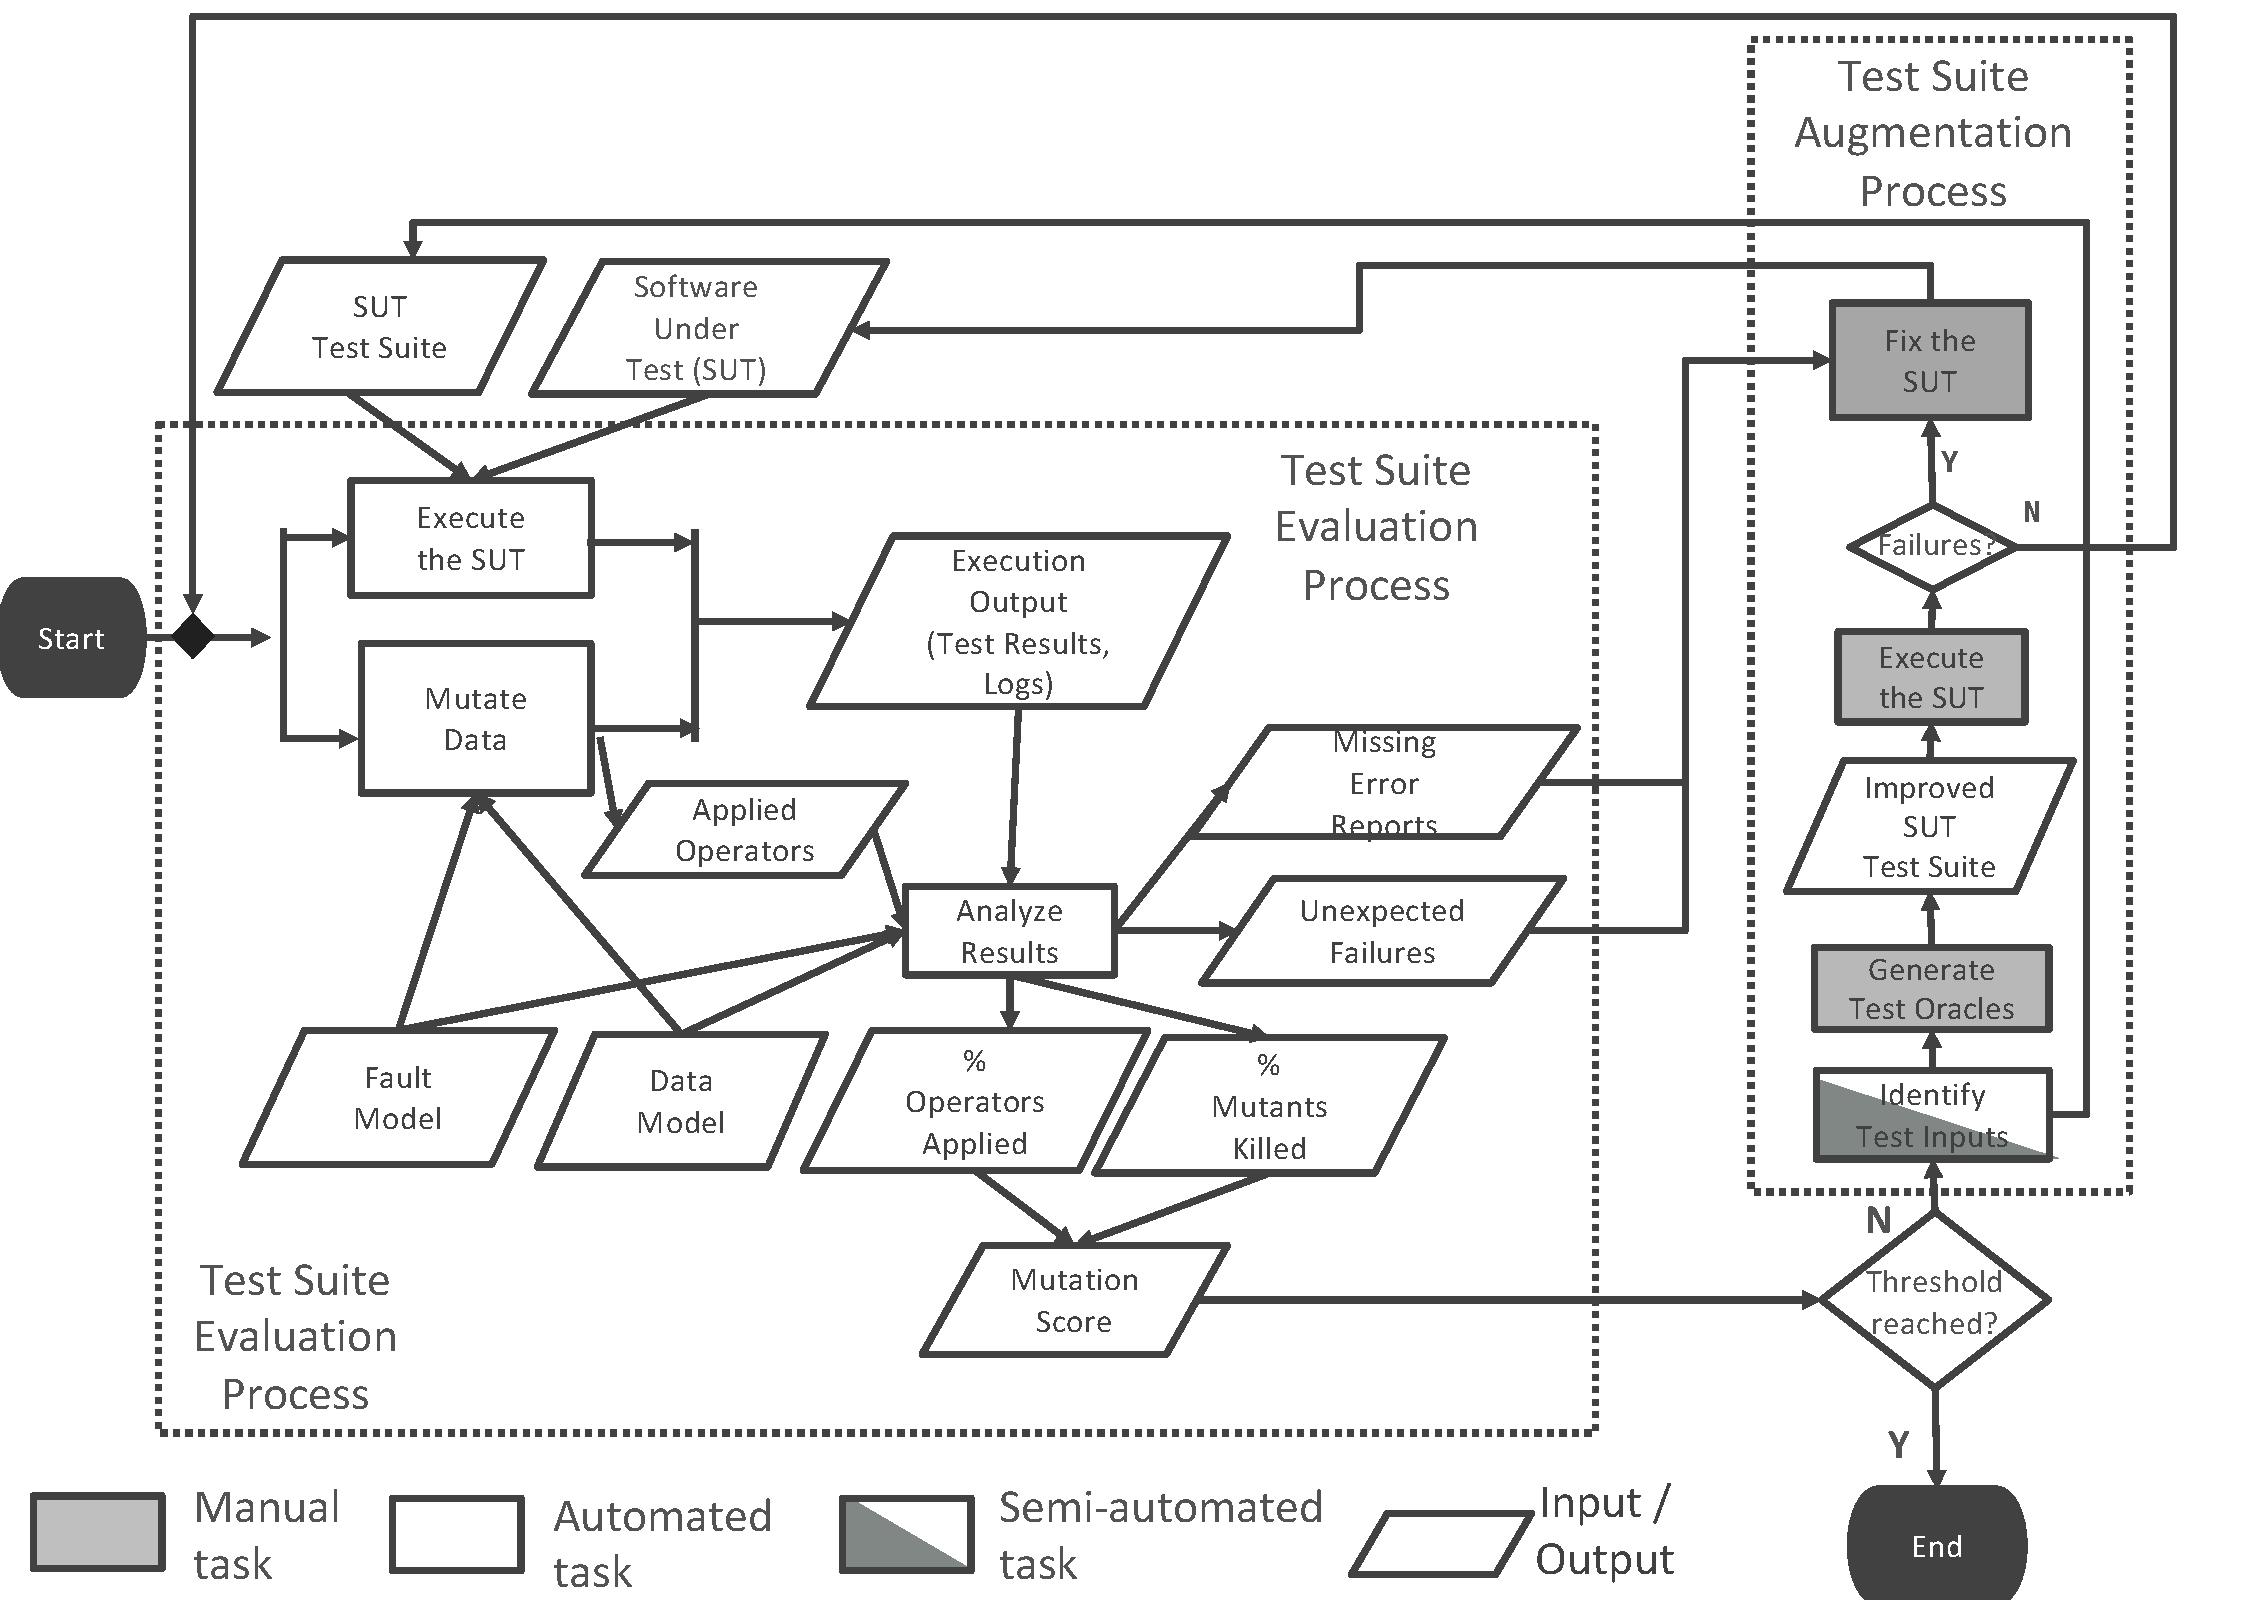
\includegraphics[width=\textwidth]{images/dataProcess}
		\caption{Data-driven Mutation Testing Process.}
		\label{fig:data:process}
	\end{figure}



This Chapter defines a test suite assessment process based on the injection of faults in the data processed by software components; we refer to this process as \INDEX{data-driven mutation testing}. 
%The definition of data-driven mutation testing is a unique contribution of this book; it has not been presented in previous literature work.

Data-driven mutation testing aims to assess test suites by simulating faults that affect the data produced, received, or exchanged by the software and its components.
It is based on a \INDEX{fault model} capturing the type of data faults that might affect the system. The fault model is produced by software engineers based on their domain knowledge and experience~\cite{di2015generating}. \MREVISION{C18}{The considered faults might be due to programming errors, hardware problems, or critical situations in the environment (e.g., noise in the channel).} The data is then automatically  mutated (i.e., modified) by a set of operators that aim to replicate the faults in the fault model. For example, the \INDEX{bit flip operator} flips a randomly selected bit of a field of the transmitted data (see Section~\ref{sec:faultModel}). 
%Mutation operators can be applied multiple times, on different data chunks or over repeated executions of a test case, ti


Figure \ref{fig:data:process} shows the reference data-driven mutation testing process that will be considered in FAQAS. The process is based on two main sub-processes, \EMPH{test suite evaluation} and \EMPH{test suite augmentation}, which are described in Sections~\ref{sec:data:test_suite_evaluation}~and~\ref{sec:data:test_suite_augmentation}, respectively. Differently from the code-driven mutation testing process introduced in Section~\ref{sec:process}, the data-driven mutation testing process has not been formalized by existing software testing literature. An extensive discussion of related work has been presented in deliverable D1.

Since data-driven mutation testing alters the data produced, received, or exchanged by the software or its components, it should be applied to evaluate test suites that trigger the execution and communication between multiple components (e.g., system or integration test cases). Data-driven mutation testing is not meant to be applied to assess unit test suites.

\clearpage
\section{Test Suite Evaluation} % (fold)
\label{sec:data:test_suite_evaluation}

The test suite evaluation process consists of three activities \EMPH{Execute the SUT}, \EMPH{Mutate Data},  and \EMPH{Analyze Results}.
The activity \INDEX{Execute the SUT} indicates that the SUT is executed against its automated test suite. 
The activity \INDEX{Mutate Data} concerns the automated modification of either the data received by the software, the data produced by the software, or the data exchanged by software components.
In Figure~\ref{fig:data:process}, the activity \EMPH{Mutate Data} is executed in parallel to the activity \EMPH{Execute the SUT} since data modification should occur at runtime during test cases execution, to simulate software faults affecting the data processed by the software.



%The fault model enables engineers to minimize the presence of equivalent mutants.
%The data model may capture the relation between inputs and outputs of the system

\begin{figure}
	\centering
		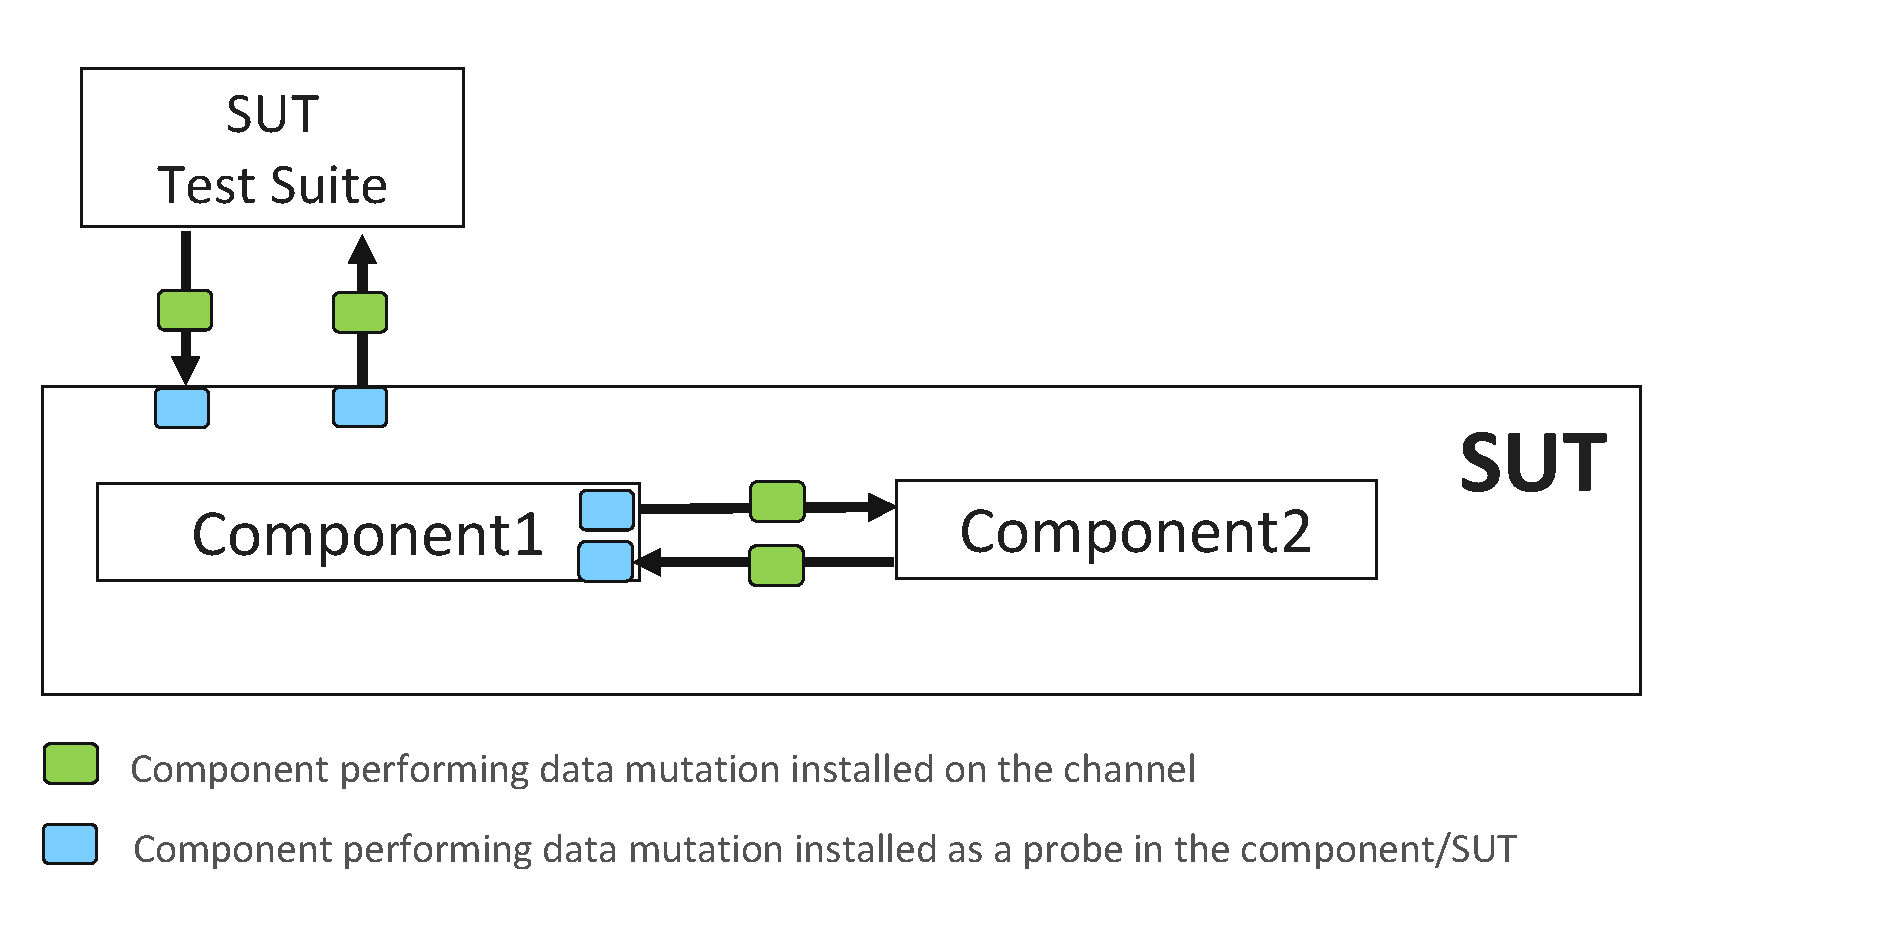
\includegraphics[width=10cm]{images/dataMutationExample}
		\caption{Example of implementation of a data mutation solution.}
		\label{fig:data:mutateData}
	\end{figure}
	
Figure~\ref{fig:data:mutateData} provides an example of how the Mutate Data activity can be implemented. Figure~\ref{fig:data:mutateData} shows that, to implement data mutation, it is necessary to integrate additional components that alter the data exchanged by the SUT components at runtime on a certain communication layer. We call such components \INDEX{mutation probes}.

An ideal target for data-driven mutation testing is the communication between loosely coupled software components; typically the ones that run on separated pieces of hardware (e.g., the on board controller and the ADCS).
In FAQAS case studies, the communication between such software components is performed by relying on APIs of a dedicated communication layer; which is typical in well designed software systems. The main functionality of such communication layer is to serialize and deserialize data that should be transmitted on the communication channel. In FAQAS case studies, the communication layer is either implemented in-house by the company that produced the case study or it is built by relying on the ASN.1 compiler architecture. In both the two cases, the communication layer implements distinct functions to serialize and deserialize data.
For this reason, in FAQAS, we expect mutation probes to be \EMPH{integrated into the software API functions that either serialize or deserialize the data being sent on the communication channel}.

In the case of a communication layer implemented in-house, we expect mutation probes to be integrated into the software under test by engineers who \EMPH{manually} add calls to the functions of a \INDEX{data-driven mutation testing API} in the source code of the software. Indeed, since communication APIs vary from system to system, it is not possible to define a tool that automatically modifies the source code or the executable code of the SUT.  Instead, we provide a \INDEX{data-driven mutation testing API} that implements the logic for mutating the data specified by the engineer.
To be applicable to a wide rande of software systems, the API will provide methods that enable mutating data buffers provided as C arrays.
Figure~\ref{fig:data:mutationProbes} shows an example of a mutation probe manually integrated into the source code (API method names begin with the prefix \emph{\_FAQAS}).

In the case of a communication layer implemented by relying on the ASN.1 compiler, the FAQAS framework will automatically introduce mutation probes into the code that deserialize data.




\begin{figure}
	\centering
		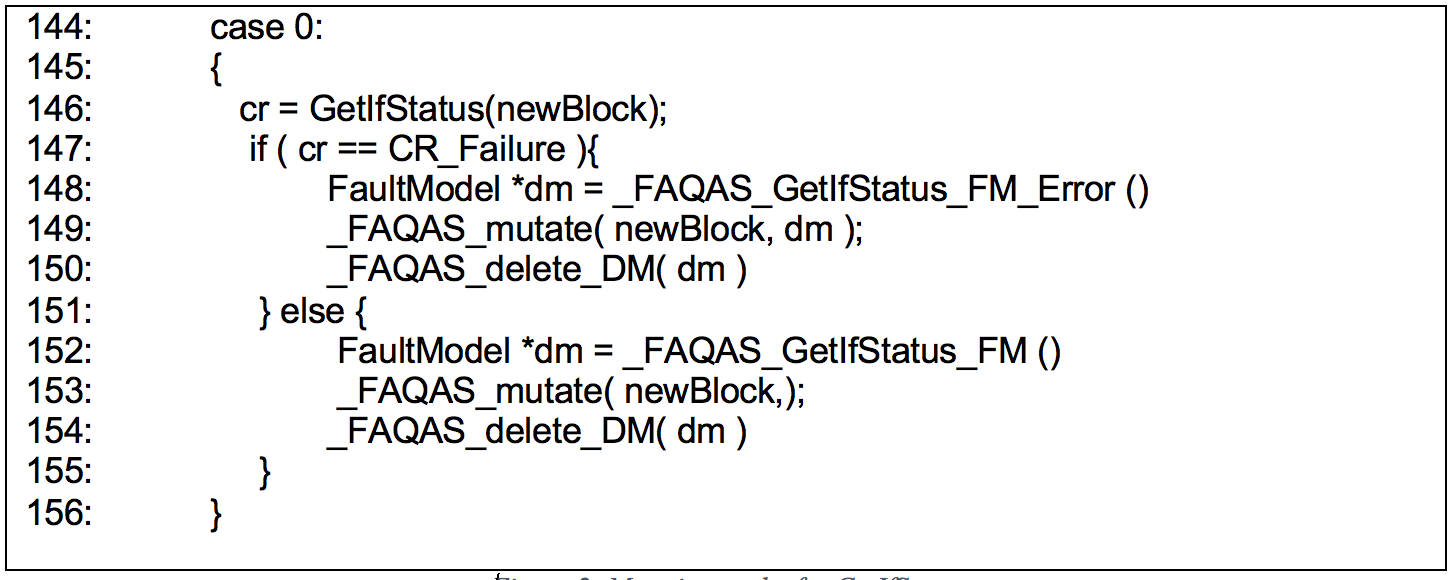
\includegraphics[width=10cm]{images/dataMutationProbes}
		\caption{Example of integration of data mutation probes.}
		\label{fig:data:mutationProbes}
	\end{figure}

%\TODO{ADD concrete example of integration}

	
%Data-driven mutation testing is driven by a faulty model specifying how to alter the data (i.e., the attributes declared in an ASN.1 grammar or the array items).	
In deliverable D1, we have clarified that, in a generic data-driven mutation testing process, the activity \EMPH{Mutate Data} may require a \INDEX{data model} that captures the characteristics and structure of the data to be mutated. 
The data model should be used to load a stream of bytes in structured form (e.g., an instance of a given data structure), which is necessary to drive data mutation. 
Also, the activity \EMPH{Mutate Data} should be driven by a \INDEX{fault model} that specifies the set of mutation operators to apply~\cite{di2015generating}. 
In FAQAS, the data model and the fault model are coupled into a same structured representation, i.e., the \INDEX{FAQAS fault model}, which is presented in Section~\ref{sec:faultModel}.


The activities \EMPH{Execute the SUT} and \EMPH{Mutate Data} are repeated till all the faults of the fault model had been applied. The possible stopping criteria are described in Section~\ref{sec:mutantsExecution}. 

The activity \INDEX{Process Outputs} processes all the outputs generated during the execution of test cases.
The collected outputs include the result of test cases execution (i.e., the list of test cases that either passed or failed) and the logs generated by the SUT during testing.
In the context of data-driven mutation testing both the \INDEX{test results} and the \INDEX{log files} are necessary to determine if a test suite kills a mutant.
Indeed, \emph{in the context of data-driven mutation testing a mutant is killed either if a test case fails, or if the software activates robustness features capable of handling the specific data fault.}
We need log files to determine if robustness features had been triggered.
For example, a system that implements a \INDEX{robust communication protocol} might simply request again the packets affected by errors thus avoiding failures. In this case, we need to inspect the log files to determine if the robustness feature had been triggered.
The fault model is expected to include only data fault classes that should either lead to failures or make the system generate an error entry in the log file.

Differently from code-driven mutation testing, data-driven mutation testing does not alter the software implementation but only the data processed by software components, for this reason it may help engineers to \INDEX{identify existing faults}, an objective that cannot be achieved by code-driven mutation testing. 
This is the case when \emph{Missing Error Reports} or \emph{Unexpected Failures }(e.g, crashes) are observed. In both the two cases, engineers should fix the system. In code-driven mutation testing, faults can be detected only after introducing new test cases that kill the generated mutants.

The activity \INDEX{Analyze Results} provides an assessment of the quality of the test suite for the SUT.
It is driven by two objectives:
\begin{itemize}
\item[(O1)] determine if the test suite is capable of detecting software faults that affect the data processed by the software components 
(e.g., we expect a test suite to fail in case the data exchanged by two components contains invalid values).
\item[(O2)] determine if the test suite exercises enough software behaviours to discover all the possible faults that may affect the data produced by the system
(i.e., it should be possible to alter the processed data to generate faulty data according to the fault model). 
\end{itemize}

\MREVISION{C19}{Objectives O1 and O2 are complementary, \REVTWO{C33}{they both should be addressed by data mutation.}
For example, a use case scenario for data-driven mutation testing could be the following: (i) data-driven mutation testing is applied to the data exchanged by \emph{component 1} and \emph{component 2} in Figure~\ref{fig:data:mutateData}, (ii) the data exchanged by the two components follow the data model in Figure~\ref{fig:DataDrivenSimpleExample}, and (iii) mutation testing is performed by applying the bit-flip mutation operator to every field of the messages being exchanged.
The data model in Figure~\ref{fig:DataDrivenSimpleExample} consists of a UML class diagram that indicates that the two components can send messages whose type can be either \emph{TimeMessage} or \emph{DataMessage}. A \emph{TimeMessage} contains only one field of type Long, which is the timestamp. 
A \emph{DataMessage} contains two fields, one field of type \emph{Integer} capturing the size of the payload, and one array of bytes containing the payload. 
Objective O1 is fulfilled when every mutant leads to the failure of least one test case.
Objective O2 is fulfilled when mutation testing generates at least (i) one \emph{TimeMessage} with field \emph{timestamp} being altered,
(ii) one \emph{DataMessage} with field \emph{size} being altered,
and (iii) one \emph{DataMessage} with field \emph{payload} being altered.
For a test suite consisting of two test cases that trigger the exchange of the messages as in the bottom-left part of Figure~\ref{fig:DataDrivenSimpleExample}, the execution of the bit flip mutation operator may lead to messages that lead to test failures. Since all the mutants are killed (i.e., the two test cases fail), objective O1 is achieved. However, the test suite does not lead to the exchange of any message of type \emph{DataMessage}, for this reason objective O2 is not achieved. Objective O2 enables us to determine that the test suite does not excercise the case in which the two components exchange messages of type \emph{DataMessage}. When data-driven mutation testing is performed against components that are expected to guarantee robustness against the exchange of erroneous data, as a by-product, objective O2 also ensures that components' robustness is properly tested.}



\REVTWO{C34}{Activity \emph{Analyze Results} concerns the automated computation of the \INDEX{mutation score} from execution data. It is 
computed as the weighted average of the percentage of mutants being killed and the percentage of mutation operators applied.}
The former enables data-driven mutation to achieve objective O1 in Section~\ref{sec:dataProcess}, the latter objective O2. 
%Details are provided in Section~\ref{sec:data:mutationscore}.

\REVTWO{C34}{Activity \emph{Analyze Results} takes as input the the data model, the fault model, the list of killed mutants, and the list of mutation operators applied.}
The list of applied mutation operators should enable engineers to determine if all the available mutation operators have been applied.


\begin{figure}[t!]
  \centering
    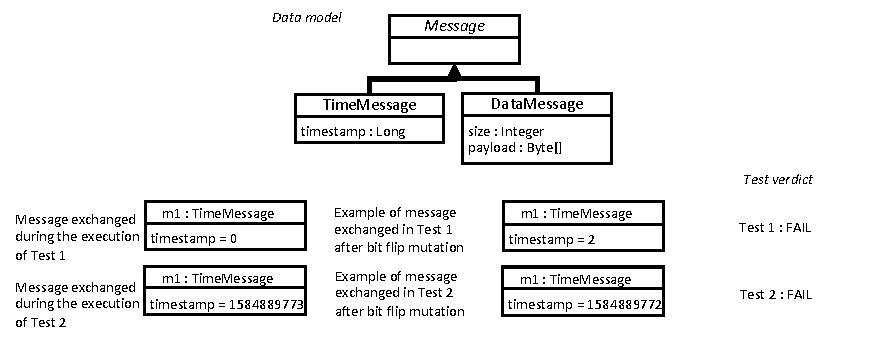
\includegraphics{images/DataDrivenSimpleExample}
      \caption{Simplified data mutation example.}
      \label{fig:DataDrivenSimpleExample}
\end{figure}

\clearpage



\clearpage
\subsection{FAQAS Fault Model}
\label{sec:dataModel}
\label{sec:faultModel}





A building block of the fault model are a set of \EMPH{data fault classes}.
A  \INDEX{data fault class} captures the type of an error that might affect the data. In turns, it specifies the mutation that should be applied in order to replace valid data with erroneous data. For each fault class we have defined a corresponding \INDEX{data mutation operator} having the same name. 
Each {data mutation operator} performs data mutation by applying a \INDEX{data mutation operation} (e.g., set a value above the upper range value). Mutation operators might apply one or more data mutation operations.
Each data mutation operator can be configured with a set of parameters. 

Table~\ref{table:faultModel:FAQAS} provides the list of data fault classes supported by FAQAS along with a description. For each fault class we indicate the data types to which it is expected to be applied, we identify four data types: 
\begin{itemize}
\item int, which indicates an integer
\item float, which indicates a floating point number
\item double, which indicates a double precision floating point number
\item bin, which indicate data that should be treated in its binary form
\end{itemize}


In FAQAS, data-driven mutation testing is performed by modifying either data that is stored in an array or in a data structure defined through the ASN.1 grammar. The following subsections describe the two distinct cases.







% !TEX root = ../MAIN.tex
\begin{table}[h]
\begin{center}
\scriptsize
\begin{tabular}{|p{2cm}|p{2cm}|p{4cm}|p{6cm}|}
\hline
\textbf{Fault Class}&\textbf{Types}&\textbf{Parameters}&\textbf{Description}\\
\hline
Value above threshold (VAT)&
\begin{minipage}{6cm}
INT\\
LONG INT\\
FLOAT\\
DOUBLE
\end{minipage}
&
\begin{minipage}{6cm}
T: threshold\\
D: delta with respect to threshold\\
\end{minipage}
&
\begin{minipage}{6cm}
The value is above a threshold T for a delta D. 

\EMPH{Data mutation operation:} The mutation is performed by replacing the current value (a number) with a value of the same type that is equal to $(T+D)$.
\end{minipage}
\\

\hline
Value below threshold (VBT)&
\begin{minipage}{6cm}
INT\\
LONG INT\\
FLOAT\\
DOUBLE
\end{minipage}
&
\begin{minipage}{6cm}
T: threshold\\
D: delta with respect to threshold\\
\end{minipage}
&
\begin{minipage}{6cm}
The value is below a threshold T for a delta D. 

\EMPH{Data mutation operation:} The mutation is performed by replacing the current value (a number) with a value of the same type that is equal to $(T-D)$.
\end{minipage}
\\



\hline
Value out of range (VOR)&
\begin{minipage}{4cm}
INT\\
LONG INT\\
FLOAT\\
DOUBLE
\end{minipage}
&
\begin{minipage}{4cm}
MIN: minimum valid value\\
MAX: maximum valid value\\
D: delta with respect to minimum/maximum valid value
\end{minipage}
&
\begin{minipage}{6cm}
The value is out of the valid range MIN-MAX. 

\EMPH{Data mutation operations (2):}  The mutation is performed by replacing the current value (a number) with 
\begin{itemize}
\item a value of the same type that is equal to $(MIN-D)$
\item a value of the same type that is equal to $(MAX+D)$
\end{itemize}
\end{minipage}
\\

\hline
Bit flip (BF)&
BIN
&
\begin{minipage}{4cm}
MIN: lower bit\\
MAX: higher bit\\
STATE: mutate only if the bit is in the given state\\
\TRFOUR{VALUE: integer specifying the number of bits to mutate}\\
\end{minipage}
&
\begin{minipage}{6cm}
A number of bits randomly chosen in the positions between MIN and MAX (included) are flipped.

\EMPH{Data mutation operation:} the operator flips N randomly selected bit.
If STATE is specified, the mutation is applied only if  the bit is in the specified state. Parameter VALUE specifies the number of bits to mutate.
\end{minipage}
\\

\hline
Invalid numeric value (INV)&
\begin{minipage}{6cm}
INT\\
LONG INT\\
FLOAT\\
DOUBLE
\end{minipage}
&
\begin{minipage}{4cm}
MIN: lower valid value\\
MAX: higher valid value\\
\TRFOUR{D: distribution to follow}\\
\TRFOUR{VALUE: mean value for normal distribution}\\
\end{minipage}
&
\begin{minipage}{6cm}
The value is legal (i.e., in the specified range) but different than the current one, which, in this case, is expected to be consistent with the status of the system.

\EMPH{Data mutation operation:} Mutation is performed by replacing the current value with a different value randomly sampled in the specified range. The parameter D specified the distribution to follow when performing the mutation\footnote{In our implementation 0 indicates uniform, 1 indicates normal around the specified value (but in range).}
\end{minipage}
\\

\hline
Illegal Value (IV)
&
\begin{minipage}{6cm}
INT\\
LONG INT\\
FLOAT\\
DOUBLE
\end{minipage}
&
\begin{minipage}{6cm}
VALUE: illegal value that is observed\\
\end{minipage}
&
\begin{minipage}{6cm}
The value is illegal and equal to the provided one (i.e., parameter \emph{VALUE}).

\EMPH{Data mutation operation:} Mutation is performed by replacing the current value with the value \emph{VALUE}, if different than the current one.
\end{minipage}
\\

\hline
\TRFOUR{Anomalous Signal Amplitude (ASA)}
&
\begin{minipage}{6cm}
INT\\
LONG INT\\
FLOAT\\
DOUBLE
\end{minipage}
&
\begin{minipage}{6cm}
T: change point\\
D: delta to add/remove\\
V: value to multiply\\
\end{minipage}
&
\begin{minipage}{6cm}
The value is modified by amplifying/reducing it by a factor V and adding or removing D from the observed value. It is used to "amplify" a signal in a constant manner to simulate unusual signal. T indicates the observed value below which instead of adding  we subtract .

\EMPH{Data mutation operation:} Mutation is performed by replacing the current value ($v$) with the value ($v'$) computed as follows:

\[
v' =  
    \begin{cases}
      T+(  (v-T)*V  ) + D   & \mathit{if}\ v \ge T\\
      T - (  (T-v)*V  ) - D   & \mathit{if}\ v < T
    \end{cases}       
\]
\end{minipage}
\\


\hline
\TRFOUR{Signal Shift (SS)}
&
\begin{minipage}{6cm}
INT\\
LONG INT\\
FLOAT\\
DOUBLE
\end{minipage}
&
\begin{minipage}{6cm}
D: delta by which the signal should be shifted\\
\end{minipage}
&
\begin{minipage}{6cm}
The value is modified by adding a value D. It simulate an anomalous shift in the signal.
\end{minipage}
\\





\hline
\TRFOUR{Hold Value (HV)}
&
\begin{minipage}{6cm}
BIN\\
INT\\
LONG INT\\
FLOAT\\
DOUBLE
\end{minipage}
&
\begin{minipage}{6cm}
V: number of times to repeat the same value\\
\end{minipage}
&
\begin{minipage}{6cm}
This operator keeps repeating an observed value for $V$ times. It emulates a constant signal replacing a signal supposed to vary.
\end{minipage}
\\



\hline
\TRFOUR{Array Swap (AS)}
&
\begin{minipage}{6cm}
ARRAY\_*\\
\end{minipage}
&
\begin{minipage}{6cm}
MIN: position of element A\\
MAX: position of element B\\
VALUE: number of elements to move\\
\end{minipage}
&
\begin{minipage}{6cm}
Replace a number of elements (number specified by VALUE) located starting from position MIN, with a number of elements located starting from position MAX, and viceversa.
\EMPH{Data mutation operation:} Mutation is performed by replacing the two set of elements with each other.
\end{minipage}
\\


\hline
\TRFOUR{Array Random Swap (ARS)}
&
\begin{minipage}{6cm}
ARRAY\_*\\
\end{minipage}
&
\begin{minipage}{6cm}
MIN: min position of element A/B\\
MAX: max position of element A/B\\
VALUE: number of elements to move\\
\end{minipage}
&
\begin{minipage}{6cm}
Replace a number of elements (number specified by VALUE) located in a position between MIN and MAX, with a number of elements located in a position between MIN and MAX. MIN and MAX specify a position with respect to the beginning and end of the array.  For example, MIN=0 indicates the first element of teh array, MIN=-2 indicates the second element of the array.
\EMPH{Data mutation operation:} Mutation is performed by replacing the two set of elements with each other.
\end{minipage}
\\



%Incorrect Identifier& Several transmission data fields have fixed values, for example fields identifying the transmitting satellite. Hardware/software errors may assign incorrect identifiers.\\
%%Incorrect Checksum& Hardware/software errors may result in an incorrect checksum for a Packet or VCDU.\\
%Incorrect Counter& Counters are used to track Packet or VCDU ordering. Hardware/software errors may assign incorrect counter values.\\
%Flipped Data Bits& Physical channel noise may flip one or more bits in the data transmission.\\
\hline
\end{tabular}
\end{center}
\caption{Data Fault Classes}
\label{table:faultModel:FAQAS}
\end{table}%

\subsubsection{Fault Model Specifications for Data Buffers}

When the data to be mutated is stored in an array, we require the definition of a fault model in the form of a block diagram since this format enables to represent the sequence of data items in the array. 
For each data block the FAQAS fault model captures its type and a list of data fault classes that might affect the block. 
The type of the data block indicates how the values of bits should be interpreted (e.g., as a floating point number). Since a data type may span over multiple items of the data buffer, for each block, we may indicate whether also the values of the following blocks should be used to load the data.

Table~\ref{table:faultModel:example} provides an example of two fault models described in tabular form. 
It resembles the CSV format supported by the FAQAS toolset. For each data item we report the span, type, and fault class. For each fault class we indicate the values of the configuration parameters for the corresponding mutation operator.


% !TEX root = ../MAIN.tex
\begin{table}[h]
\begin{center}
\small
\begin{tabular}{|p{1cm}|p{2cm}|p{1cm}|p{1cm}|p{1cm}|p{1cm}|p{1cm}|p{2cm}|p{1cm}|p{1cm}|}
\hline
\textbf{Fault Model Name}&\textbf{DataItem}&\textbf{Span}&\textbf{Type}&\textbf{Fault Class}&\textbf{Min}&\textbf{Max}&\textbf{Threshold}&\textbf{Delta}&\textbf{State}\\
\hline
IfHK&0&1&BIN&BF&0&0&-&-&-\\
IfHK&1&1&INT&VOR&0&5&-&1&-\\
IfHK&2&2&BIN&BF&0&63&-&-&-\\
IfHK&4&1&BIN&BF&0&0&-&-&-\\
\hline
IfStatus&0&1&BIN&BF&0&0&-&-&-\\
\hline
\end{tabular}
\end{center}
\caption{Driven Fault Model Buffer}
\label{table:faultModel:example}
\end{table}%

\clearpage
\subsubsection{Fault Model Specifications for ASN.1 grammar}

The ASN.1 grammar enables engineers to specify data structures where the types of the items in the data structure are selected from a predefined set.

%When the data to be mutated is stored in a data structure defined through the ASN.1 grammar, the fault model is specified by indicating which operators to apply on the specific fields of the data structure. 

We have identified a set of feasible fault classes for each type supported by the ASN1CC compiler.
The corresponding mutation operators are automatically configured based on the ASN.1 grammar (e.g., in the case of an attribute of type INTEGER, the min/max values of the VOR operator are derived from the boundaries of the INTEGER type).
Table~\ref{table:faultModel:FAQAS:ASN1} provides, for each of such types, the feasible fault classes and the configurations for the mutation operators.
In the configuration for the mutation operators, we refer to the variables (e.g., MIN and MAX) appearing in the ASN1 xml file.

Figure~\ref{fig:ASN1ProbesGeneration} provides an overview of the process in place to generate probes including the fault model.
The engineer first export the ASN.1 grammar as XML, then he modifies the generated file by specifying, for each \emph{Asn1Type}, the mutation operator to be used (this is done by adding an xml attribute called \emph{MutationOperator} with a value specifying the name of the operator). The engineer can tune the mutation by changing the value ranges associated to the different types. For example, this could be done to restrict the valid range of an INTEGER from (MIN=-100, MAX=100) to a nominal range of (MIN=0,MAX=50).
In case a data type is defined through value range constraints, the FAQAS framework will configure one mutation operator for each range.

% !TEX root = ../MAIN.tex
\begin{table}[h]
\begin{center}
\small
\begin{tabular}{|p{2cm}|p{2cm}|p{4cm}|p{4cm}|}
\hline
\textbf{Types}&\textbf{Fault Classes}&\textbf{Parameters}&\textbf{Description}\\
\hline
INTEGER&
VAT&
\begin{minipage}{4cm}
T: MAX\\
D: 1\\
\end{minipage}
&
\begin{minipage}{4cm}
\end{minipage}
\\
\hline
INTEGER&
VBT&
\begin{minipage}{4cm}
T: MIN\\
D: 1\\
\end{minipage}
&
\begin{minipage}{4cm}
\end{minipage}
\\
\hline
INTEGER&
VOR&
\begin{minipage}{4cm}
MIN: MIN\\
MAX: MAX\\
D: 1\\
\end{minipage}
&
\begin{minipage}{4cm}
\end{minipage}
\\
\hline
REAL&
VAT&
\begin{minipage}{4cm}
T: MAX\\
D: 1\\
\end{minipage}
&
\begin{minipage}{4cm}
\end{minipage}
\\
\hline
REAL&
VBT&
\begin{minipage}{4cm}
T: MIN\\
D: 1\\
\end{minipage}
&
\begin{minipage}{4cm}
\end{minipage}
\\
\hline
REAL&
VOR&
\begin{minipage}{4cm}
MIN: MIN\\
MAX: MAX\\
D: 1\\
\end{minipage}
&
\begin{minipage}{4cm}
\end{minipage}
\\
\hline
ENUMERATED&
INV&
\begin{minipage}{4cm}
MIN: MIN\\
MAX: MAX\\
D: 1\\
\end{minipage}
&
\begin{minipage}{4cm}
\end{minipage}
\\
\hline
BOOLEAN&
BF&
\begin{minipage}{4cm}
MIN: 0\\
MAX: 0\\
\end{minipage}
&
\begin{minipage}{4cm}
\end{minipage}
\\
\hline
NULL&
BF&
\begin{minipage}{4cm}
MIN: 0\\
MAX: 0\\
\end{minipage}
&
\begin{minipage}{4cm}
\end{minipage}
\\
\hline
BIT STRING&
BF&
\begin{minipage}{4cm}
MIN: 0\\
MAX: 0\\
\end{minipage}
&
\begin{minipage}{4cm}
\end{minipage}
\\
\hline
OCTET STRING&
BF&
\begin{minipage}{4cm}
MIN: 0\\
MAX: 0\\
\end{minipage}
&
\begin{minipage}{4cm}
\end{minipage}
\\
\hline
IA5STRING&
BF&
\begin{minipage}{4cm}
MIN: 0\\
MAX: 0\\
\end{minipage}
&
\begin{minipage}{4cm}
\end{minipage}
\\
\hline
NUMERIC STRING&
BF&
\begin{minipage}{4cm}
MIN: 0\\
MAX: 0\\
\end{minipage}
&
\begin{minipage}{4cm}
\end{minipage}
\\
\hline
SEQUENCE&
-&
\begin{minipage}{4cm}
\end{minipage}
&
\begin{minipage}{4cm}
No mutation environed for this type.
\end{minipage}
\\
\hline
SET&
-&
\begin{minipage}{4cm}
\end{minipage}
&
\begin{minipage}{4cm}
No mutation environed for this type.
\end{minipage}
\\
\hline
CHOICE&
-&
\begin{minipage}{4cm}
\end{minipage}
&
\begin{minipage}{4cm}
No mutation environed for this type.
\end{minipage}
\\
\hline
SEQUENCE OF&
-&
\begin{minipage}{4cm}
\end{minipage}
&
\begin{minipage}{4cm}
No mutation environed for this type.
\end{minipage}
\\
\hline
SET OF&
-&
\begin{minipage}{4cm}
\end{minipage}
&
\begin{minipage}{4cm}
No mutation environed for this type.
\end{minipage}
\\



%Incorrect Identifier& Several transmission data fields have fixed values, for example fields identifying the transmitting satellite. Hardware/software errors may assign incorrect identifiers.\\
%%Incorrect Checksum& Hardware/software errors may result in an incorrect checksum for a Packet or VCDU.\\
%Incorrect Counter& Counters are used to track Packet or VCDU ordering. Hardware/software errors may assign incorrect counter values.\\
%Flipped Data Bits& Physical channel noise may flip one or more bits in the data transmission.\\
\hline
\end{tabular}
\end{center}
\caption{Data Fault Classes for ASN.1 data types.}
\label{table:faultModel:FAQAS:ASN1}
\end{table}%



\begin{figure}[tb]
  \centering
    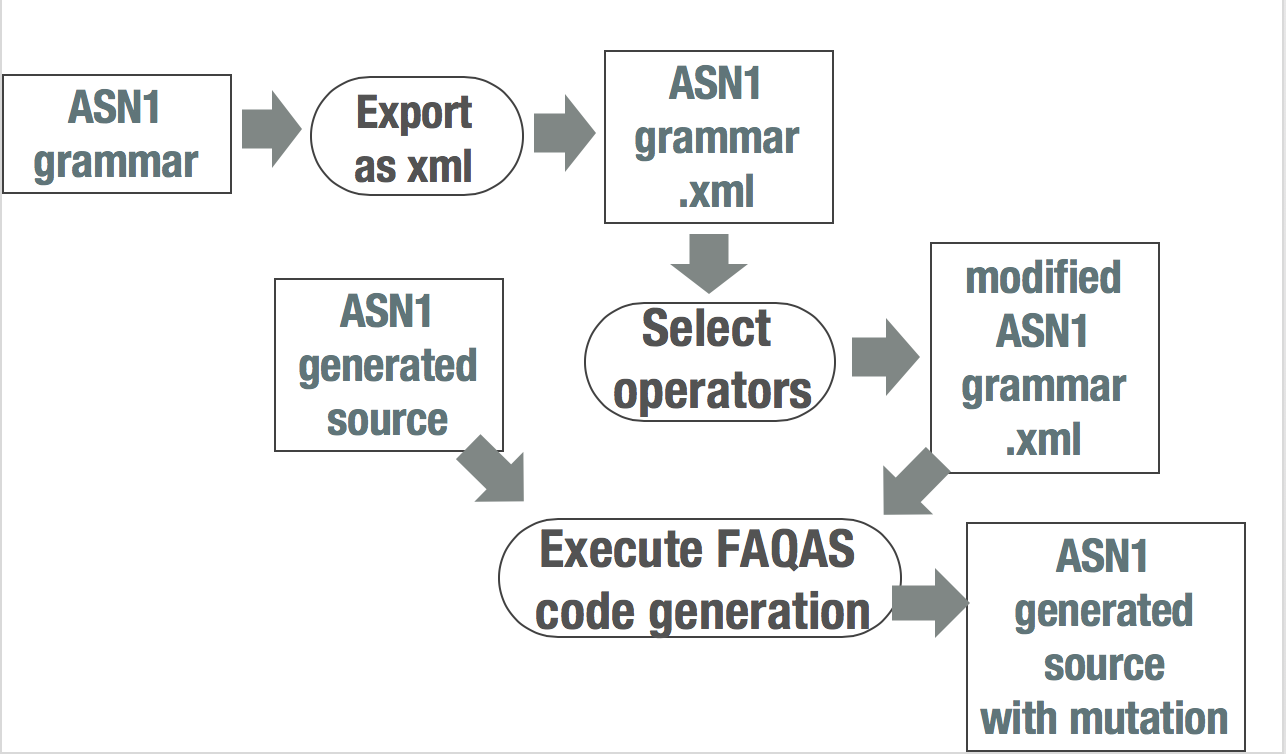
\includegraphics[width=12cm]{images/ASN1mutationProces}
      \caption{Data-driven probes generation process for ASN1.}
      \label{fig:ASN1ProbesGeneration}
\end{figure}








\clearpage
\subsection{FAQAS Data Mutation API and Probes}
\label{sec:FAQASDataMutationProbes}

In FAQAS, the data-driven mutation testing API is automatically generated from the fault model provided by engineers. Data mutation probes are either manually implemented by software engineers (in the case data mutation should target an ad-hoc communication layer that works with data buffers) or automatically generated by the toolset (in the case data mutation should target an ASN.1-based communication layer).

Section~\ref{sec:FAQASDataMutationProbesBuffer} describes the case of data buffers (i.e., C arrays).
Section~\ref{sec:FAQASDataMutationProbesASN} describes the case of ASN.1.


\subsubsection{Data Mutation for Data Buffers}
\label{sec:FAQASDataMutationProbesBuffer}

Figure~\ref{fig:DataDrivenBufferProcess} provides an overview of the envisioned data mutation process. 
The engineer prepares a single specification file for all the fault models that work with data buffers of a same time (e.g., int). The fault model specification is used by the FAQAS generator to automatically generate the mutation API. The engineer, then, modifies the source code of the SUT to add invocations to the mutation probes provided by the FAQAS API. 

Finally, the engineer iteratively executes the compiler in a loop to generate a different executable of the SUT for each mutation operation to perform.
The source code of the SUT is the same for all the fault models working on a data buffer of the same type. A configuration option (i.e., a \emph{define directive}) passed to the compiler is what drives the configuration of the specific mutation operation to be performed. 
More precisely, the engineer executes the compiled with the directive \EMPH{-DMUTATIONOPT=i}, where \emph{i} is a value between 0 and \emph{max}. The value \emph{max} coincides with the
overall number of mutation operation instances. An \INDEX{instance of a mutation operation} is a mutation operation that belongs to a mutation operator defined for a specific data item of the fault model. For the fault model in Table in \ref{table:faultModel:example} we have 6 instances, one for each data item except for data item 2, whose VOR fault class includes two mutation operations.

\begin{figure}[tb]
  \centering
    \includegraphics{images/DataDrivenBufferProcess}
      \caption{Data-driven mutation process for buffered data.}
      \label{fig:DataDrivenBufferProcess}
\end{figure}

The code that invokes the automatically generated probe is manually inserted by the engineer as shown in Listing~\ref{probesExample}.
The logic of the mutation probes is predefined and shared by all the mutation probes. What determines the different behaviours is the fault model.
The definition of the fault model is automatically generated in a \EMPH{C struct} (see Listing~\ref{faultModelExample}). 
The backbone data structures are predefined an provided in Listing~\ref{faultModelStructure}.

The code of the mutation probe is shown in Listing~\ref{mutationProbe}. It works by identifying the data item to mutate, the mutation operator to apply, and the mutation operation to execute by invoking methods \EMPH{\_FAQAS\_selectItem},
\EMPH{\_FAQAS\_selectOperator}, and \EMPH{\_FAQAS\_selectOperation}, respectively. The implementation of these three methods is automatically generated based on the fault model definition file.
An example is shown in Listing~\ref{selectors}. The runtime behaviour depends on the variable \EMPH{MUTATION}, whose value depends on the option passed at compile time. 
The variable \EMPH{MUTATION} uniquely identifies an instance of a mutation operation.
% (i.e., a mutation operation that belongs to a mutation operator defined for a specific data item of the fault model).

% !TEX root =  ../MAIN.tex

\begin{minipage}{15cm}
\begin{lstlisting}[style=CStyle, caption=Example of a data-driven mutation probes., label=probesExample, mathescape=true]


int receiveData()
{

    std::vector<char> v = connectAndReceiveData(); //function that receives data

    //MANUALLY ADDED PROBE
    FaultModel *fm = _FAQAS_IfHK_FM();
    _FAQAS_mutate(v->data(),fm);
    //MANUALLY ADDED PROBE END


}
\end{lstlisting}
\end{minipage}



% !TEX root =  ../MAIN.tex

\begin{minipage}{15cm}
\begin{lstlisting}[style=CStyle, caption=Example of generated fault models in C., label=faultModelExample, mathescape=true]
#define SIZE_IfHK 4
#define SIZE_IfStatus 1


struct FaultModel* _FAQAS_IfHK_FM(){
FaultModel *fm = _FAQAS_create_FM(SIZE_IfHK);

fm->items[0].operators[0].type=BF;
fm->items[0].operators[0].min=0;
fm->items[0].operators[0].max=0;
fm->items[0].operators[0].state=-1;
fm->items[0].operatorsN=1;
fm->items[0].span=1;
fm->items[0].type=BIN;

fm->items[1].operators[0].type=VOR;
fm->items[1].operators[0].min=0;
fm->items[1].operators[0].max=5;
fm->items[1].operators[0].delta=1;
fm->items[1].operatorsN=1;
fm->items[1].span=1;
fm->items[1].type=INT;

fm->items[2].operators[0].type=BF;
fm->items[2].operators[0].min=0;
fm->items[2].operators[0].max=0;
fm->items[2].operators[0].state=-1;
fm->items[2].operatorsN=1;
fm->items[2].span=2;
fm->items[2].type=BIN;

fm->items[4].operators[0].type=BF;
fm->items[4].operators[0].min=0;
fm->items[4].operators[0].max=0;
fm->items[4].operators[0].state=-1;
fm->items[4].operatorsN=1;
fm->items[4].span=1;
fm->items[4].type=BIN;
return fm;
}
struct FaultModel* _FAQAS_IfStatus_FM(){
FaultModel *fm = _FAQAS_create_FM(SIZE_IfStatus);

fm->items[0].operators[0].type=BF;
fm->items[0].operators[0].min=0;
fm->items[0].operators[0].max=0;
fm->items[0].operators[0].state=-1;
fm->items[0].operatorsN=1;
fm->items[0].span=1;
fm->items[0].type=BIN;
return fm;
}
\end{lstlisting}
\end{minipage}



% !TEX root =  ../MAIN.tex

\begin{minipage}{15cm}
\begin{lstlisting}[style=CStyle, caption=Fault model data structures., label=faultModelStructure, mathescape=true]
#define MAX_OPS 10
#define ITEMS 10


int MUTATION=MUTATIONOPT;

enum DataType {
    INT,
    FLOAT,
    DOUBLE,
    BIN
};

enum MutationType{
    BF,
    IV,
    VOR,
    VAT,
    VBT,
    INV
};

int _FAQAS_mutated = 0;

struct MutationOperator {
    MutationType type;
    int min;
    int max;
    int delta;
    int state;
};

struct DataItem {
    DataType type;
    int span;
    int operatorsN;
    struct MutationOperator operators[MAX_OPS];
};

struct FaultModel {
    int itemsN;
    struct DataItem *items;
};

\end{lstlisting}
\end{minipage}



% !TEX root =  ../MAIN.tex

\begin{minipage}{15cm}
\begin{lstlisting}[style=CStyle, caption=Automatically generated selectors., label=selectors, mathescape=true]
int _FAQAS_selectItem(FaultModel *dm){
if ( MUTATION == 0 )
    return 0;
if ( MUTATION == 1 )
    return 1;
if ( MUTATION == 2 )
    return 1;
if ( MUTATION == 3 )
    return 2;
if ( MUTATION == 4 )
    return 4;
if ( MUTATION == 5 )
    return 0;
}
int _FAQAS_selectOperator(FaultModel *dm){
if ( MUTATION == 0 )
    return 0;
if ( MUTATION == 1 )
    return 0;
if ( MUTATION == 2 )
    return 0;
if ( MUTATION == 3 )
    return 0;
if ( MUTATION == 4 )
    return 0;
if ( MUTATION == 5 )
    return 0;
}
int _FAQAS_selectOperation(FaultModel *dm){
if ( MUTATION == 0 )
    return 0;
if ( MUTATION == 1 )
    return 0;
if ( MUTATION == 2 )
    return 1;
if ( MUTATION == 3 )
    return 0;
if ( MUTATION == 4 )
    return 0;
if ( MUTATION == 5 )
    return 0;
}
\end{lstlisting}
\end{minipage}



% !TEX root =  ../MAIN.tex

\begin{minipage}{15cm}
\begin{lstlisting}[style=CStyle, caption=Mutation API function., label=mutationProbe, mathescape=true]
int _FAQAS_mutate( int *data, FaultModel *fm ){
    if ( _FAQAS_mutated == 1 )
    return 0;

    if ( MUTATION == -1 )
    return 0;

    int pos = _FAQAS_selectItem(fm);
    int op = _FAQAS_selectOperator(fm);
    int opt = _FAQAS_selectOperation(fm);

    int valueInt;
    int valueBin;
    double valueDouble;


    //Load the data in the appripriate var
    if ( fm->items[pos].type == BIN ){
        valueBin = (int) data[pos];
    }
    if ( fm->items[pos].type == INT ){
        valueInt = (int) data[pos];
    }
    if ( fm->items[pos].type == DOUBLE ){
        valueDouble = (double) data[pos];
    }
...
    MutationOperator *OP = &(fm->items[pos].operators[op]);    
...     
        if ( OP->type == VOR ){
        if ( fm->items[pos].type == INT ){

            if ( opt == 0 ){
                valueInt = OP->min-OP->delta;
            } else if (opt == 1 ){
                valueInt = OP->max+OP->delta;
            } else {
                //ERROR
            }
            _FAQAS_mutated = 1;
        }

...

    }

...

    if ( _FAQAS_mutated != 1 ){
        return 0;
    }

    //
    //Store the data
    //
    //FIXME: handle span
    if ( fm->items[pos].type == INT ){
        data[pos] = valueInt;
    }
    if ( fm->items[pos].type == DOUBLE ){
        data[pos] = valueDouble;
    }
    if ( fm->items[pos].type == BIN ){
        data[pos] = valueBin;
    }
    
    ...

    
\end{lstlisting}
\end{minipage}




\subsubsection{Data Mutation Probes for ASN.1}
\label{sec:FAQASDataMutationProbesASN}

\TODO{This section still needs to be written. We may put a sequence diagram that show that at the beginning the probe loads the info about the mutation operation instance to execute and execute it if feasible.}

\clearpage
\subsection{Test suite execution}
\label{sec:mutantsExecution}

During data mutation the test suite is executed a number of times that depends on a stopping criterion chosen by the engineer. We foresee two possible stopping criteria (1) every test case is run with every data mutation operation (hereafter, test coverage stopping criterion)
%, (2) exercise each data fault class (hereafter, fault coverage stopping criterion)
, and (2) a sample of the available data mutation operations has been executed with every test case (hereafter, sampling stopping criterion).

% !TEX root =  ../Main.tex

%\newcommand{\INDA}{10}
%\newcommand{\INDB}{15}
%\newcommand{\INDC}{5}

%\vspace{-3mm}
\begin{figure}[tb]

\begin{algorithmic}[1]

%\footnotesize
\scriptsize
\Require \emph{EMOS}, set of SUT executables, each one implementing one mutation operation (EMO)
\Require \emph{TS}, the test suite of the SUT
% (source inputs, follow-up inputs, output data).


\State \hspace{5 mm} \textbf{for each} $t$ in $TS$ \label{alg:prioritize:prel}
\State \hspace{10 mm} \textbf{execute} $t$ to track the data items exercised by t

\State \textbf{for each} $EMO$ in $EMO$ \label{alg:dataProcess:repeat}
\State \hspace{5 mm} \textbf{for each} $t$ in $TS$ \label{alg:prioritize:t}
\State \hspace{10 mm} \textbf{if} $t$ contains a data item that can be mutated with $EMO$ \label{alg:prioritize:cove}
\State \hspace{15 mm} \textbf{execute} $t$ with $EMO$
\State \hspace{15 mm} \textbf{if} $t$ fails or invalid data detected
\State \hspace{\INDB mm} \textbf{break} \label{alg:prioritize:stop}



\end{algorithmic}
\vspace{-3mm}
\caption{Algorithm for executing data-driven mutation testing with test coverage stopping criterion}
%\vspace{-0.2cm}
\label{alg:dataProcess}
\end{figure}




Figure~\ref{alg:dataProcess} shows how the data mutation process should be iterated with
 the \EMPH{test coverage stopping criterion}. 

A preliminary execution of the test suite against a mutated executable configured to simply track the data items exchanged during each test case execution (Line~\ref{alg:prioritize:prel}), enable us to determine which test cases exercise the data items targeted by a specific mutation operation instance.

 For each mutation operation instance (Line~\ref{alg:dataProcess:repeat}), we execute every test case of the test suite (Line~\ref{alg:prioritize:t}), if it exercise the data item targeted by the mutation operation (Line~\ref{alg:prioritize:cove}), till one of the test cases kills the mutant, i.e., it fails or detects the presence of invalid data and trigger a fault tolerant mechanism (Line~\ref{alg:prioritize:stop}).
 We can configure the data mutation API to inject a single data fault or to mutate all the data where the mutation operation instance can be applied (this is useful to simulate a bit that is always flipped because of hardware fault).
The mutation algorithm can either mutate the first mutable data item observed or randomly decide whether to mutate the mutable data item. The second case enables the mutation of data items exchanged after long components interactions. However, it requires the repeated execution of a test case in case the mutation has not been performed but a data item could have been mutated. 



%With the fault coverage stopping criterion the full test suite is executed multiple times till all the possible data fault classes had been injected at least once (for the full test suite).
%A data fault class is no longer injected after it has already been injected in a test case of the test suite.
%The mutation algorithm can either mutate the first mutable data item observed or randomly decide whether to mutate the mutable data item.
%The repeated execution of a test case is terminated after it has been executed once without identifying any mutable data item.

With the \EMPH{sampling stopping criterion} we perform the same activities performed for the test coverage criterion except that the set of mutation operation instances to be performed is randomly sampled (e.g., only 5\% of the mutation operations are considered).



\clearpage
\section{Test Suite Augmentation} % (fold)
\label{sec:data:test_suite_augmentation}

\TODO{This section still needs to be written.}

%The test suite augmentation process concerns the definition of additional test cases to increase the mutation score.
%It consists of four activities \emph{Identify Test Inputs}, \emph{Generate Test Oracles}, \emph{Execute the SUT}, \emph{Fix the SUT}. 
%Despite these activities match the ones performed in the case of code-driven mutation testing, they are triggered and implemented in a different manner, as described below.
%
%
%
%In the presence of mutants not killed by test cases (i.e., when the \emph{\% of Mutants Killed} is not equal to 100\%), engineers are expected to improve the oracles of existing test cases. Indeed, the presence of mutants not killed by test cases indicates that the oracles of the test suite are not capable of detecting that the software is failing. 
%Automated approaches for performing this activity in the presence of system or integration test suites are not available and thus it needs to be performed manually.
%
%In the presence of operators not being applied (i.e., the \emph{\% Operators Applied} is not equal to 100\%), engineers are expected to generate new test inputs for the SUT that enable the application of all the mutation operators. 
%For example, in the case of the example in Figure~\ref{fig:DataDrivenSimpleExample}, engineers would need to implement test cases that trigger the exchange of \emph{DataMessages}.
%Fully automated approaches to generate test cases for data-driven mutation testing are unavailable; however, techniques that generate input data from scratch~\cite{gligoric2010test} or augment input data~\cite{DiNardo:TOSEM:2017} can be adopted. 
%Also, when the data used by test cases is generated by simulators, meta-heuristic search can be used to drive the generation of input data~\cite{Abdessalem:ICSE:2018}. 
%
%The execution of the SUT and the repair of the SUT are performed manually as in the case of code-driven data mutation.
%
%
%\TODO{Clarify if we generate test cases or not}
%
%Section~\ref{sec:testGenerationData} provides details about the existing solutions to  \emph{Identify Test Inputs} and \emph{Generate Test Oracles}.




% !TEX root = MutationTestingSurvey.tex

\chapter{Mutation Testing Benchmarks}
\label{chapter:industry}

In Section~\ref{sec:limitations} we have provided an overview of state-of the-art solutions to perform mutation testing and address limitations of the mutation testing process.
Each of these solutions had been evaluated against a set of case study systems deemed representative for the usage context. Such case study systems consist of a software under test (SUT) and a test suite for the software.
Hereafter, we'll use the term \INDEX{benchmark} to indicate the set of case study systems used in the empirical evaluation presented in a research paper.
%introduce an empirical evaluation aimed to prove or disprove a specific theory proposed by the authors. 
These benchmarks can be used as reference for future mutation testing developments. 
Also, a deep understanding of the characteristics of the benchmarks considered in the literature, may provide insights on the generalizability of the results to space software (e.g, results evaluated against a real time application are more likely generalizable to the case of space software).


% !TEX root =  ../MutationTestingSurvey.tex

\setlength\LTleft{0pt}
\setlength\LTright{0pt}
\scriptsize 
\begin{longtable}{@{\extracolsep{\fill}}|p{1.2cm}|p{6cm}|p{4.3cm}|p{1.2cm}|@{}}
\caption{\normalsize List of conferences and journals considered in our survey.}
\label{table:papers} \\
\hline

	\textbf{Acronym} & \textbf{Name}	&	\textbf{\begin{tabular}[c]{@{}l@{}}Type of Venue\\(Conference Proceedings, Journal)\end{tabular}}	&	\textbf{Publisher}\\

\hline
	ICST & International Conference on Software Testing, Validation and Verification &	Conference Proceedings	&	IEEE\\
	ICSTW & International Conference on Software Testing, Verification and Validation Workshops &	Conference Proceedings	&	IEEE\\
	ICSE & International Conference on Software Engineering &	Conference Proceedings	&	IEEE/ACM\\
	ASE & International Conference on Automated Software Engineering & Conference Proceedings	& IEEE/ACM\\
	ISSTA & International Symposium on Software Testing and Analysis & Conference Proceedings	&	ACM\\
	TSE & Transactions on Software Engineering & Journal	&	IEEE\\
	%TOSEM & Transactions on Software Engineering and Methodology & Journal	& ACM\\
	TR & Transactions on Reliability & Journal & IEEE\\
	IST & Information and Software Technology & Journal	&	Elsevier\\
	SCP & Science of Computer Programming & Journal	&	Elsevier\\
	STVR & Software Testing, Verification and Reliability & Journal	&	Wiley\\
\hline                                                           
\end{longtable}
\normalsize


In this chapter we provide a survey of the benchmarks considered in empirical evaluations described in research work presented in top software engineering conferences and journals, between 2013 and 2019. Table~\ref{table:papers} provides the list of conferences and journals considered in our survey. For every venue, we have considered all the empirical evaluations considering C and C++ case study systems. Table~\ref{table:papers} provides the acronym and name of the venue, the type of venue, i.e., whether if it is a journal of a conference proceedings, and finally the publisher of the venue. 

%\DONE{Add the table of conferences, describe the columns in the text. Columns should be: name, type of venue (conference proceedings,journal),publisher.}

%\DONE{I rewrote, I do not expect you to introduce a table. You may have writte someting like "In this section we describe of the most relevant benchmarks targeting C software systems, they are summarized in Table..". I rewrote differently.}

\REVTWO{C40}{In the following, we introduce Sections~\ref{section:industry:code} and~\ref{section:industry:data}, which present detailed information about benchmarks on code-driven and data-driven mutation testing, respectively.}

%\DONE{check the date}

\section{Code-Driven Mutation Testing Benchmarks}
\label{section:industry:code}

% !TEX root = MAIN.tex

\chapter{Software Validation Process Planning}

\subsection{General}

The approach followed to validate the \FAQAS is to apply it to different case studies provided by LuxSpace and GOMSpace.
Table~\ref{tab:caseStudies} provides the list of case studies along with an indication of the type of mutation testing (i.e., code-driven or data-driven) they will be targeted for. More information on the case studies are present in the \emph{D2}.

\begin{table}[htp]
\caption{Case studies for the FAQAS activity.}
\label{tab:caseStudies}
\begin{center}
\begin{tabular}{|p{1.2cm}|p{6cm}|p{2.5cm}|p{2.5cm}|}
\hline
\textbf{Partner}&\textbf{Case study}&\textbf{Code-driven}&\textbf{Data-driven}\\
\hline
LXS&System Test Suite for ESAIL&Y&Y\\
LXS&Unit Test Suite for ESAIL&Y&N\\
GSL&Unit Test Suite for libUtil&Y&N\\
GSL&Integration Test Suite for libgscsp&Y&Y\\
GSL&System Test Suite for libparam&Y&Y\\
ESA&MLFS mathematical library&Y&N\\
ESA&ASN1 Compiler&Y&N\\
\hline
\end{tabular}
\end{center}
\end{table}

\clearpage


Table~\ref{table:case_studies} provides the list of the case study systems considered in the literature. For each case study we report (1) the case study (i.e., the software under test - SUT), (2) the size of the SUT (the size may vary according to the specific study), (3) the size of the test suite for the SUT\footnote{The size may vary from an empirical evaluation to another; also, in some cases the test suite details were not available (N/A).} (4) the number of papers that report using the case study, and (5) the references to the papers that report the case study.

%\DONE{You have to describe what types of programs it contains, when it was developed.}

From Table~\ref{table:case_studies} can be seen that the Siemens, Make and Space are the most common case studies with 6, 5 and 4 uses, respectively. 
The most used case study is the \INDEX{Siemens suite}. The programs belonging to this suite are commonly used to evaluate state-of-the-art solutions because they it includes faulty versions affected by faults introduced by engineers during development. The suite is available through the Subject Infrastructure Repository (SIR) from the University of Nebraska-Lincoln\footnote{https://sir.csc.ncsu.edu/portal/index.php}, in particular the suite contains a diverse collection of C programs that include code involving integer and floating-point operations, pointers, memory allocation, loops and complex conditional expressions.The Siemens suite was introduced in 1994 by Hutchins et al.~\cite{hutchins1994experiments}, the programs from the suite come with a large pool of test cases written initially by Hutchins et al. and then augmented by Rothermel et al.~\cite{rothermel1998empirical}.

Table~\ref{table:benchmarks} provides the list of benchmarks identified in the literature. We report (1) the case studies of the benchmark (i.e., the software under test - SUT), (2) the size of SUT in terms of lines of code (LOC), (3) the size of the SUT test suite in terms of number of test cases, (4) the original goal of the evaluation, and (5) the actual reference to the paper in which the benchmark was originally presented. 



%\DONE{"Appreciate" is a little too much :)}
%From Table~\ref{table:benchmarks}, it also can be appreciated the wide variety of case studies selected in the literature, while some authors decide to assess their techniques using very simple programs such as \textit{abs}~\cite{tokumoto2016muvm}. Other authors preferred using Unix applications such as the Coreutils package~\cite{hariri2019comparing,papadakis2018mutation,chekam2017empirical}. 
%On the other hand, some authors selected very complex programs such as OpenSSL and LLVM~\cite{denisov2018mull}, but usually the experiments are exercised only on small components of these large applications.

The size of the benchmark case studies varies a lot. They include simple algorithms such as \textit{abs} (6 LOC)~\cite{tokumoto2016muvm}, large Unix utilities such as the Coreutils package~\cite{hariri2019comparing,papadakis2018mutation,chekam2017empirical}, and programs implementing complex functions such as OpenSSL and LLVM~\cite{denisov2018mull}.
However, when large and complex software systems are considered in the empirical evaluation, the evaluation concerns only a subset of the components of these large applications.
For example, in the study performed by Kintis et al.~\cite{kintis2017detecting} they considered the assessment of Vim, a Unix text editor of 362 KLOC, however, because of the size of the program, the authors decided to restrict the analysis only to a couple of components such as \texttt{spell} and \texttt{eval}, 16 and 22 KLOC, respectively. 

%\DONE{Provide an example. Describe what they did in a paper where they selected a component, otherwise the sentence above might not be understood}

Concerning the size of the selected software under test, the most relevant studies have been presented by Papadakis and Chekam~\cite{papadakis2018mutation,chekam2017empirical,papadakis2018mutant}. Specifically, these authors considered the case studies Coreutils, Findutils, Grep, Make and Codeflaws (83 KLOC, 18 KLOC, 9 KLOC, 35 KLOC and 266 KLOC respectively). 
Concerning the size of the test suite employed to assess their adequacy, again Papadakis and Chekam~\cite{papadakis2018mutation,chekam2017empirical,papadakis2018mutant} present the most comprehensive studies with test suite sizes ranging from 58\,131, to 122\,261 test cases.
Despite scalability remains an open problem for mutation testing, the work of Papadakis and Chekam~\cite{papadakis2018mutation,chekam2017empirical,papadakis2018mutant} shows that optimization techniques are scaling up to large software systems.

Concerning the adoption of \INDEX{industrial case studies}, the most recent work is that of \cite{delgado2018evaluation} where mutation testing has been applied to 15 functions of a Commercial Off The Shelf Component used in nuclear systems. 
Another paper evaluating the applicability of mutation testing to safety critical systems is that of Daran and Thavenod-Fosse~\cite{daran1996software}, who conducted a study to identify if mutations are correlated with real faults; the experimentation was carried out on a critical software from the civil nuclear field. Andrews et al.~\cite{andrews2005mutation}, who explored the relation between hand-seeded and real faults in the Space software. Space is a software developed at the European Space Agency that it has been used as case study in software engineering papers since 1998 \cite{frankl1998further}.
Baker and Habli~\cite{baker2012empirical} conducted experiments on two safety-critical airborne systems, C and Ada, that had satisfied the coverage requirements for certification. In their experiments, they found an effective subset of mutation operators able to detect multiple deficiencies in test suites already assessed by experts. 

\REVTWO{C41}{Even though, many efforts has been done to make code-driven mutation testing a scalable solution, we conclude from this benchmark section, that unfortunately no study has yet applied mutation testing to complex and large real industrial software. Furthermore, in the context of space software, the applicability of mutation testing on large-scale satellite systems has not been empirically evaluated yet.}

\REVTWO{C42}{From this section, we conclude that mutation testing as a technique is applied mainly within research environments, and that in particular, mutation testing has not been adopted formally within industrial software development environments.}

% carried out an empirical evaluation based on two safety-critical airborne systems that had satisfied the coverage requirements for certification. Those systems were developed using high-integrity subsets for C (MISRA C [33]) and Ada. In their experiments, they found an effective subset of mutation operators that was able to detect different deficiencies in tests suites which had already met statement and MC/DC coverage and had been manually peer-reviewed.

% !TEX root = MutationTestingSurvey.tex

\chapter{Mutation Testing Benchmarks}
\label{chapter:industry}

In Section~\ref{sec:limitations} we have provided an overview of state-of the-art solutions to perform mutation testing and address limitations of the mutation testing process.
Each of these solutions had been evaluated against a set of case study systems deemed representative for the usage context. Such case study systems consist of a software under test (SUT) and a test suite for the software.
Hereafter, we'll use the term \INDEX{benchmark} to indicate the set of case study systems used in the empirical evaluation presented in a research paper.
%introduce an empirical evaluation aimed to prove or disprove a specific theory proposed by the authors. 
These benchmarks can be used as reference for future mutation testing developments. 
Also, a deep understanding of the characteristics of the benchmarks considered in the literature, may provide insights on the generalizability of the results to space software (e.g, results evaluated against a real time application are more likely generalizable to the case of space software).


% !TEX root =  ../MutationTestingSurvey.tex

\setlength\LTleft{0pt}
\setlength\LTright{0pt}
\scriptsize 
\begin{longtable}{@{\extracolsep{\fill}}|p{1.2cm}|p{6cm}|p{4.3cm}|p{1.2cm}|@{}}
\caption{\normalsize List of conferences and journals considered in our survey.}
\label{table:papers} \\
\hline

	\textbf{Acronym} & \textbf{Name}	&	\textbf{\begin{tabular}[c]{@{}l@{}}Type of Venue\\(Conference Proceedings, Journal)\end{tabular}}	&	\textbf{Publisher}\\

\hline
	ICST & International Conference on Software Testing, Validation and Verification &	Conference Proceedings	&	IEEE\\
	ICSTW & International Conference on Software Testing, Verification and Validation Workshops &	Conference Proceedings	&	IEEE\\
	ICSE & International Conference on Software Engineering &	Conference Proceedings	&	IEEE/ACM\\
	ASE & International Conference on Automated Software Engineering & Conference Proceedings	& IEEE/ACM\\
	ISSTA & International Symposium on Software Testing and Analysis & Conference Proceedings	&	ACM\\
	TSE & Transactions on Software Engineering & Journal	&	IEEE\\
	%TOSEM & Transactions on Software Engineering and Methodology & Journal	& ACM\\
	TR & Transactions on Reliability & Journal & IEEE\\
	IST & Information and Software Technology & Journal	&	Elsevier\\
	SCP & Science of Computer Programming & Journal	&	Elsevier\\
	STVR & Software Testing, Verification and Reliability & Journal	&	Wiley\\
\hline                                                           
\end{longtable}
\normalsize


In this chapter we provide a survey of the benchmarks considered in empirical evaluations described in research work presented in top software engineering conferences and journals, between 2013 and 2019. Table~\ref{table:papers} provides the list of conferences and journals considered in our survey. For every venue, we have considered all the empirical evaluations considering C and C++ case study systems. Table~\ref{table:papers} provides the acronym and name of the venue, the type of venue, i.e., whether if it is a journal of a conference proceedings, and finally the publisher of the venue. 

%\DONE{Add the table of conferences, describe the columns in the text. Columns should be: name, type of venue (conference proceedings,journal),publisher.}

%\DONE{I rewrote, I do not expect you to introduce a table. You may have writte someting like "In this section we describe of the most relevant benchmarks targeting C software systems, they are summarized in Table..". I rewrote differently.}

\REVTWO{C40}{In the following, we introduce Sections~\ref{section:industry:code} and~\ref{section:industry:data}, which present detailed information about benchmarks on code-driven and data-driven mutation testing, respectively.}

%\DONE{check the date}

\section{Code-Driven Mutation Testing Benchmarks}
\label{section:industry:code}

% !TEX root = MAIN.tex

\chapter{Software Validation Process Planning}

\subsection{General}

The approach followed to validate the \FAQAS is to apply it to different case studies provided by LuxSpace and GOMSpace.
Table~\ref{tab:caseStudies} provides the list of case studies along with an indication of the type of mutation testing (i.e., code-driven or data-driven) they will be targeted for. More information on the case studies are present in the \emph{D2}.

\begin{table}[htp]
\caption{Case studies for the FAQAS activity.}
\label{tab:caseStudies}
\begin{center}
\begin{tabular}{|p{1.2cm}|p{6cm}|p{2.5cm}|p{2.5cm}|}
\hline
\textbf{Partner}&\textbf{Case study}&\textbf{Code-driven}&\textbf{Data-driven}\\
\hline
LXS&System Test Suite for ESAIL&Y&Y\\
LXS&Unit Test Suite for ESAIL&Y&N\\
GSL&Unit Test Suite for libUtil&Y&N\\
GSL&Integration Test Suite for libgscsp&Y&Y\\
GSL&System Test Suite for libparam&Y&Y\\
ESA&MLFS mathematical library&Y&N\\
ESA&ASN1 Compiler&Y&N\\
\hline
\end{tabular}
\end{center}
\end{table}

\clearpage


Table~\ref{table:case_studies} provides the list of the case study systems considered in the literature. For each case study we report (1) the case study (i.e., the software under test - SUT), (2) the size of the SUT (the size may vary according to the specific study), (3) the size of the test suite for the SUT\footnote{The size may vary from an empirical evaluation to another; also, in some cases the test suite details were not available (N/A).} (4) the number of papers that report using the case study, and (5) the references to the papers that report the case study.

%\DONE{You have to describe what types of programs it contains, when it was developed.}

From Table~\ref{table:case_studies} can be seen that the Siemens, Make and Space are the most common case studies with 6, 5 and 4 uses, respectively. 
The most used case study is the \INDEX{Siemens suite}. The programs belonging to this suite are commonly used to evaluate state-of-the-art solutions because they it includes faulty versions affected by faults introduced by engineers during development. The suite is available through the Subject Infrastructure Repository (SIR) from the University of Nebraska-Lincoln\footnote{https://sir.csc.ncsu.edu/portal/index.php}, in particular the suite contains a diverse collection of C programs that include code involving integer and floating-point operations, pointers, memory allocation, loops and complex conditional expressions.The Siemens suite was introduced in 1994 by Hutchins et al.~\cite{hutchins1994experiments}, the programs from the suite come with a large pool of test cases written initially by Hutchins et al. and then augmented by Rothermel et al.~\cite{rothermel1998empirical}.

Table~\ref{table:benchmarks} provides the list of benchmarks identified in the literature. We report (1) the case studies of the benchmark (i.e., the software under test - SUT), (2) the size of SUT in terms of lines of code (LOC), (3) the size of the SUT test suite in terms of number of test cases, (4) the original goal of the evaluation, and (5) the actual reference to the paper in which the benchmark was originally presented. 



%\DONE{"Appreciate" is a little too much :)}
%From Table~\ref{table:benchmarks}, it also can be appreciated the wide variety of case studies selected in the literature, while some authors decide to assess their techniques using very simple programs such as \textit{abs}~\cite{tokumoto2016muvm}. Other authors preferred using Unix applications such as the Coreutils package~\cite{hariri2019comparing,papadakis2018mutation,chekam2017empirical}. 
%On the other hand, some authors selected very complex programs such as OpenSSL and LLVM~\cite{denisov2018mull}, but usually the experiments are exercised only on small components of these large applications.

The size of the benchmark case studies varies a lot. They include simple algorithms such as \textit{abs} (6 LOC)~\cite{tokumoto2016muvm}, large Unix utilities such as the Coreutils package~\cite{hariri2019comparing,papadakis2018mutation,chekam2017empirical}, and programs implementing complex functions such as OpenSSL and LLVM~\cite{denisov2018mull}.
However, when large and complex software systems are considered in the empirical evaluation, the evaluation concerns only a subset of the components of these large applications.
For example, in the study performed by Kintis et al.~\cite{kintis2017detecting} they considered the assessment of Vim, a Unix text editor of 362 KLOC, however, because of the size of the program, the authors decided to restrict the analysis only to a couple of components such as \texttt{spell} and \texttt{eval}, 16 and 22 KLOC, respectively. 

%\DONE{Provide an example. Describe what they did in a paper where they selected a component, otherwise the sentence above might not be understood}

Concerning the size of the selected software under test, the most relevant studies have been presented by Papadakis and Chekam~\cite{papadakis2018mutation,chekam2017empirical,papadakis2018mutant}. Specifically, these authors considered the case studies Coreutils, Findutils, Grep, Make and Codeflaws (83 KLOC, 18 KLOC, 9 KLOC, 35 KLOC and 266 KLOC respectively). 
Concerning the size of the test suite employed to assess their adequacy, again Papadakis and Chekam~\cite{papadakis2018mutation,chekam2017empirical,papadakis2018mutant} present the most comprehensive studies with test suite sizes ranging from 58\,131, to 122\,261 test cases.
Despite scalability remains an open problem for mutation testing, the work of Papadakis and Chekam~\cite{papadakis2018mutation,chekam2017empirical,papadakis2018mutant} shows that optimization techniques are scaling up to large software systems.

Concerning the adoption of \INDEX{industrial case studies}, the most recent work is that of \cite{delgado2018evaluation} where mutation testing has been applied to 15 functions of a Commercial Off The Shelf Component used in nuclear systems. 
Another paper evaluating the applicability of mutation testing to safety critical systems is that of Daran and Thavenod-Fosse~\cite{daran1996software}, who conducted a study to identify if mutations are correlated with real faults; the experimentation was carried out on a critical software from the civil nuclear field. Andrews et al.~\cite{andrews2005mutation}, who explored the relation between hand-seeded and real faults in the Space software. Space is a software developed at the European Space Agency that it has been used as case study in software engineering papers since 1998 \cite{frankl1998further}.
Baker and Habli~\cite{baker2012empirical} conducted experiments on two safety-critical airborne systems, C and Ada, that had satisfied the coverage requirements for certification. In their experiments, they found an effective subset of mutation operators able to detect multiple deficiencies in test suites already assessed by experts. 

\REVTWO{C41}{Even though, many efforts has been done to make code-driven mutation testing a scalable solution, we conclude from this benchmark section, that unfortunately no study has yet applied mutation testing to complex and large real industrial software. Furthermore, in the context of space software, the applicability of mutation testing on large-scale satellite systems has not been empirically evaluated yet.}

\REVTWO{C42}{From this section, we conclude that mutation testing as a technique is applied mainly within research environments, and that in particular, mutation testing has not been adopted formally within industrial software development environments.}

% carried out an empirical evaluation based on two safety-critical airborne systems that had satisfied the coverage requirements for certification. Those systems were developed using high-integrity subsets for C (MISRA C [33]) and Ada. In their experiments, they found an effective subset of mutation operators that was able to detect different deficiencies in tests suites which had already met statement and MC/DC coverage and had been manually peer-reviewed.

% !TEX root = MutationTestingSurvey.tex

\chapter{Mutation Testing Benchmarks}
\label{chapter:industry}

In Section~\ref{sec:limitations} we have provided an overview of state-of the-art solutions to perform mutation testing and address limitations of the mutation testing process.
Each of these solutions had been evaluated against a set of case study systems deemed representative for the usage context. Such case study systems consist of a software under test (SUT) and a test suite for the software.
Hereafter, we'll use the term \INDEX{benchmark} to indicate the set of case study systems used in the empirical evaluation presented in a research paper.
%introduce an empirical evaluation aimed to prove or disprove a specific theory proposed by the authors. 
These benchmarks can be used as reference for future mutation testing developments. 
Also, a deep understanding of the characteristics of the benchmarks considered in the literature, may provide insights on the generalizability of the results to space software (e.g, results evaluated against a real time application are more likely generalizable to the case of space software).


\input{tables/papers}

In this chapter we provide a survey of the benchmarks considered in empirical evaluations described in research work presented in top software engineering conferences and journals, between 2013 and 2019. Table~\ref{table:papers} provides the list of conferences and journals considered in our survey. For every venue, we have considered all the empirical evaluations considering C and C++ case study systems. Table~\ref{table:papers} provides the acronym and name of the venue, the type of venue, i.e., whether if it is a journal of a conference proceedings, and finally the publisher of the venue. 

%\DONE{Add the table of conferences, describe the columns in the text. Columns should be: name, type of venue (conference proceedings,journal),publisher.}

%\DONE{I rewrote, I do not expect you to introduce a table. You may have writte someting like "In this section we describe of the most relevant benchmarks targeting C software systems, they are summarized in Table..". I rewrote differently.}

\REVTWO{C40}{In the following, we introduce Sections~\ref{section:industry:code} and~\ref{section:industry:data}, which present detailed information about benchmarks on code-driven and data-driven mutation testing, respectively.}

%\DONE{check the date}

\section{Code-Driven Mutation Testing Benchmarks}
\label{section:industry:code}

\input{tables/case_studies}

Table~\ref{table:case_studies} provides the list of the case study systems considered in the literature. For each case study we report (1) the case study (i.e., the software under test - SUT), (2) the size of the SUT (the size may vary according to the specific study), (3) the size of the test suite for the SUT\footnote{The size may vary from an empirical evaluation to another; also, in some cases the test suite details were not available (N/A).} (4) the number of papers that report using the case study, and (5) the references to the papers that report the case study.

%\DONE{You have to describe what types of programs it contains, when it was developed.}

From Table~\ref{table:case_studies} can be seen that the Siemens, Make and Space are the most common case studies with 6, 5 and 4 uses, respectively. 
The most used case study is the \INDEX{Siemens suite}. The programs belonging to this suite are commonly used to evaluate state-of-the-art solutions because they it includes faulty versions affected by faults introduced by engineers during development. The suite is available through the Subject Infrastructure Repository (SIR) from the University of Nebraska-Lincoln\footnote{https://sir.csc.ncsu.edu/portal/index.php}, in particular the suite contains a diverse collection of C programs that include code involving integer and floating-point operations, pointers, memory allocation, loops and complex conditional expressions.The Siemens suite was introduced in 1994 by Hutchins et al.~\cite{hutchins1994experiments}, the programs from the suite come with a large pool of test cases written initially by Hutchins et al. and then augmented by Rothermel et al.~\cite{rothermel1998empirical}.

Table~\ref{table:benchmarks} provides the list of benchmarks identified in the literature. We report (1) the case studies of the benchmark (i.e., the software under test - SUT), (2) the size of SUT in terms of lines of code (LOC), (3) the size of the SUT test suite in terms of number of test cases, (4) the original goal of the evaluation, and (5) the actual reference to the paper in which the benchmark was originally presented. 



%\DONE{"Appreciate" is a little too much :)}
%From Table~\ref{table:benchmarks}, it also can be appreciated the wide variety of case studies selected in the literature, while some authors decide to assess their techniques using very simple programs such as \textit{abs}~\cite{tokumoto2016muvm}. Other authors preferred using Unix applications such as the Coreutils package~\cite{hariri2019comparing,papadakis2018mutation,chekam2017empirical}. 
%On the other hand, some authors selected very complex programs such as OpenSSL and LLVM~\cite{denisov2018mull}, but usually the experiments are exercised only on small components of these large applications.

The size of the benchmark case studies varies a lot. They include simple algorithms such as \textit{abs} (6 LOC)~\cite{tokumoto2016muvm}, large Unix utilities such as the Coreutils package~\cite{hariri2019comparing,papadakis2018mutation,chekam2017empirical}, and programs implementing complex functions such as OpenSSL and LLVM~\cite{denisov2018mull}.
However, when large and complex software systems are considered in the empirical evaluation, the evaluation concerns only a subset of the components of these large applications.
For example, in the study performed by Kintis et al.~\cite{kintis2017detecting} they considered the assessment of Vim, a Unix text editor of 362 KLOC, however, because of the size of the program, the authors decided to restrict the analysis only to a couple of components such as \texttt{spell} and \texttt{eval}, 16 and 22 KLOC, respectively. 

%\DONE{Provide an example. Describe what they did in a paper where they selected a component, otherwise the sentence above might not be understood}

Concerning the size of the selected software under test, the most relevant studies have been presented by Papadakis and Chekam~\cite{papadakis2018mutation,chekam2017empirical,papadakis2018mutant}. Specifically, these authors considered the case studies Coreutils, Findutils, Grep, Make and Codeflaws (83 KLOC, 18 KLOC, 9 KLOC, 35 KLOC and 266 KLOC respectively). 
Concerning the size of the test suite employed to assess their adequacy, again Papadakis and Chekam~\cite{papadakis2018mutation,chekam2017empirical,papadakis2018mutant} present the most comprehensive studies with test suite sizes ranging from 58\,131, to 122\,261 test cases.
Despite scalability remains an open problem for mutation testing, the work of Papadakis and Chekam~\cite{papadakis2018mutation,chekam2017empirical,papadakis2018mutant} shows that optimization techniques are scaling up to large software systems.

Concerning the adoption of \INDEX{industrial case studies}, the most recent work is that of \cite{delgado2018evaluation} where mutation testing has been applied to 15 functions of a Commercial Off The Shelf Component used in nuclear systems. 
Another paper evaluating the applicability of mutation testing to safety critical systems is that of Daran and Thavenod-Fosse~\cite{daran1996software}, who conducted a study to identify if mutations are correlated with real faults; the experimentation was carried out on a critical software from the civil nuclear field. Andrews et al.~\cite{andrews2005mutation}, who explored the relation between hand-seeded and real faults in the Space software. Space is a software developed at the European Space Agency that it has been used as case study in software engineering papers since 1998 \cite{frankl1998further}.
Baker and Habli~\cite{baker2012empirical} conducted experiments on two safety-critical airborne systems, C and Ada, that had satisfied the coverage requirements for certification. In their experiments, they found an effective subset of mutation operators able to detect multiple deficiencies in test suites already assessed by experts. 

\REVTWO{C41}{Even though, many efforts has been done to make code-driven mutation testing a scalable solution, we conclude from this benchmark section, that unfortunately no study has yet applied mutation testing to complex and large real industrial software. Furthermore, in the context of space software, the applicability of mutation testing on large-scale satellite systems has not been empirically evaluated yet.}

\REVTWO{C42}{From this section, we conclude that mutation testing as a technique is applied mainly within research environments, and that in particular, mutation testing has not been adopted formally within industrial software development environments.}

% carried out an empirical evaluation based on two safety-critical airborne systems that had satisfied the coverage requirements for certification. Those systems were developed using high-integrity subsets for C (MISRA C [33]) and Ada. In their experiments, they found an effective subset of mutation operators that was able to detect different deficiencies in tests suites which had already met statement and MC/DC coverage and had been manually peer-reviewed.

\input{tables/industry}

\clearpage

\section{Data-Driven Mutation Testing Benchmarks}
\label{section:industry:data}

In this section we provide a survey of the benchmarks considered both in empirical evaluations described in research work and in industrial cases for data-driven mutation testing.

Table~\ref{table:benchmarks_datadriven} provides the list of the case study systems considered in the literature and industry. Similar to the previous section, for each case study we report (1) the case study (i.e., the software under test - SUT), (2) the size of the SUT (the size can be expressed in terms of bytecode instructions, lines of code (LOC), or executable size (KB or MB)), (3) the size of the test suite for the SUT (unfortunately, in most cases the test suite details were not available (N/A)), and (4) the references to the papers that report the case study.

Table~\ref{table:benchmarks_datadriven} presents case studies that were applied to UML models~\cite{di2017augmenting}, block models~\cite{pham2016model} and grammars~\cite{AFL:industrialcases}.

Concerning the size and typology of SUT, the case studies reported in Table~\ref{table:benchmarks_datadriven} varies a lot.
For instance, experimentation on block models has been applied to different types of desktop applications such as VLC, Adobe Reader, Real Player, and Windows Media Player~\cite{pham2016model} which sizes goes from 60 KB to 2.32 MB. 

Experimentation on grammars has been widely studied, but for sake of simplicity we only reported the most important case studies for AFL tool~\cite{AFL:industrialcases}. Particularly, AFL has been applied to a very wide range of software typology, for example it has been applied on programming languages such as PHP, web browsers such as Firefox, libraries such as OpenSSL, and even application server such as MySQL Server. 

Regarding case studies applied to space context software, we highlight SES-DAQ, a DAQ system developed by SES that processes bytestreams of transmitted satellite data. The version of SES-DAQ used for the experimentation performed by Di Nardo et al.~\cite{di2017augmenting} had a size of 32\,469 bytecode instructions.

\input{tables/industry_datadriven}




\clearpage

\section{Data-Driven Mutation Testing Benchmarks}
\label{section:industry:data}

In this section we provide a survey of the benchmarks considered both in empirical evaluations described in research work and in industrial cases for data-driven mutation testing.

Table~\ref{table:benchmarks_datadriven} provides the list of the case study systems considered in the literature and industry. Similar to the previous section, for each case study we report (1) the case study (i.e., the software under test - SUT), (2) the size of the SUT (the size can be expressed in terms of bytecode instructions, lines of code (LOC), or executable size (KB or MB)), (3) the size of the test suite for the SUT (unfortunately, in most cases the test suite details were not available (N/A)), and (4) the references to the papers that report the case study.

Table~\ref{table:benchmarks_datadriven} presents case studies that were applied to UML models~\cite{di2017augmenting}, block models~\cite{pham2016model} and grammars~\cite{AFL:industrialcases}.

Concerning the size and typology of SUT, the case studies reported in Table~\ref{table:benchmarks_datadriven} varies a lot.
For instance, experimentation on block models has been applied to different types of desktop applications such as VLC, Adobe Reader, Real Player, and Windows Media Player~\cite{pham2016model} which sizes goes from 60 KB to 2.32 MB. 

Experimentation on grammars has been widely studied, but for sake of simplicity we only reported the most important case studies for AFL tool~\cite{AFL:industrialcases}. Particularly, AFL has been applied to a very wide range of software typology, for example it has been applied on programming languages such as PHP, web browsers such as Firefox, libraries such as OpenSSL, and even application server such as MySQL Server. 

Regarding case studies applied to space context software, we highlight SES-DAQ, a DAQ system developed by SES that processes bytestreams of transmitted satellite data. The version of SES-DAQ used for the experimentation performed by Di Nardo et al.~\cite{di2017augmenting} had a size of 32\,469 bytecode instructions.

% !TEX root =  ../MutationTestingSurvey.tex


\setlength\LTleft{0pt}
\setlength\LTright{0pt}
\small 
\begin{longtable}{@{\extracolsep{\fill}}|p{4cm}|p{3.5cm}|p{3cm}|p{1.8cm}|@{}}
\caption{\normalsize Summary of Data-Driven Mutation Testing Benchmarks.}
\label{table:benchmarks_datadriven} \\

\hline

\textbf{Case Study (SUT)}	&	\textbf{Size of SUT}	&	\textbf{\begin{tabular}[c]{@{}l@{}}Size of Test Suite\\(test cases)\end{tabular}}	 & \textbf{Reference}	\\
\hline

SES-DAQ & 32\,469 bytecode instructions & 32 & \cite{di2017augmenting,di2015evolutionary,di2015generating} \\

VLC 2.0.7 & 184 KB & N/A & \cite{pham2016model} \\
Libpng 1.5.4 & 176 KB & N/A & \cite{pham2016model} \\
XnView 1.98 & 4.46 MB & N/A & \cite{pham2016model} \\
Adobe Reader 9.2& 2.32 MB & N/A & \cite{pham2016model} \\
Windows Media Player 9.0 & 1.22 MB & N/A & \cite{pham2016model} \\
Real Player SP 1.0 & 60 KB & N/A & \cite{pham2016model} \\
MIDI Player 0.35& 336 KB & N/A & \cite{pham2016model} \\
Orbital Viewer 1.04 & 538 KB & N/A & \cite{pham2016model} \\

PHP 5.4.36 & 735 KLOC & N/A & \cite{AFL:industrialcases}\\
Firefox 32.0.1 & 62 MB & N/A & \cite{AFL:industrialcases}\\
OpenSSL 1.0.2 & 264 KLOC & N/A & \cite{AFL:industrialcases}\\
PuTTY 0.54 & 68 KLOC & N/A & \cite{AFL:industrialcases}\\
MySQL Server 5.7 & 373 MB & N/A & \cite{AFL:industrialcases}\\
indent 2.2.11 & 24 KLOC & N/A & \cite{AFL:industrialcases}\\

HotelRS & 1.5 KLOC & 33  & \cite{Appelt:SQLI:ISSTA:2014}\\
Sugar-CRM & 352 KLOC & 33 & \cite{Appelt:SQLI:ISSTA:2014}\\

JavaScript Interpreter (IE7) & 113\,562 machine instructions& 2\,800 & \cite{Godefroid:GrammarBasedFuzzying:2008}\\

\textbf{Windows NT utilities}
\begin{minipage}[t]{2.5cm}
attrib\\
chkdsk\\
comp\\
expand\\
fc\\
find\\
help\\
label\\
replace\\
\end{minipage}
 & 
 \begin{minipage}[t]{2.5cm}
 \hfill\\
21 KB\\
25 KB\\
25 KB\\
65 KB\\
24 KB\\
17 KB\\
12 KB\\
17 KB\\
21 KB\\
\end{minipage}
 &  \begin{minipage}[t]{2.5cm}
 \hfill\\
 N/A
\end{minipage} &  \begin{minipage}[t]{2.5cm}
 \hfill\\
 \cite{ghosh1998testing}
\end{minipage}\\
 

\hline                                                           
\end{longtable}


\normalsize




\clearpage

\section{Data-Driven Mutation Testing Benchmarks}
\label{section:industry:data}

In this section we provide a survey of the benchmarks considered both in empirical evaluations described in research work and in industrial cases for data-driven mutation testing.

Table~\ref{table:benchmarks_datadriven} provides the list of the case study systems considered in the literature and industry. Similar to the previous section, for each case study we report (1) the case study (i.e., the software under test - SUT), (2) the size of the SUT (the size can be expressed in terms of bytecode instructions, lines of code (LOC), or executable size (KB or MB)), (3) the size of the test suite for the SUT (unfortunately, in most cases the test suite details were not available (N/A)), and (4) the references to the papers that report the case study.

Table~\ref{table:benchmarks_datadriven} presents case studies that were applied to UML models~\cite{di2017augmenting}, block models~\cite{pham2016model} and grammars~\cite{AFL:industrialcases}.

Concerning the size and typology of SUT, the case studies reported in Table~\ref{table:benchmarks_datadriven} varies a lot.
For instance, experimentation on block models has been applied to different types of desktop applications such as VLC, Adobe Reader, Real Player, and Windows Media Player~\cite{pham2016model} which sizes goes from 60 KB to 2.32 MB. 

Experimentation on grammars has been widely studied, but for sake of simplicity we only reported the most important case studies for AFL tool~\cite{AFL:industrialcases}. Particularly, AFL has been applied to a very wide range of software typology, for example it has been applied on programming languages such as PHP, web browsers such as Firefox, libraries such as OpenSSL, and even application server such as MySQL Server. 

Regarding case studies applied to space context software, we highlight SES-DAQ, a DAQ system developed by SES that processes bytestreams of transmitted satellite data. The version of SES-DAQ used for the experimentation performed by Di Nardo et al.~\cite{di2017augmenting} had a size of 32\,469 bytecode instructions.

% !TEX root =  ../MutationTestingSurvey.tex


\setlength\LTleft{0pt}
\setlength\LTright{0pt}
\small 
\begin{longtable}{@{\extracolsep{\fill}}|p{4cm}|p{3.5cm}|p{3cm}|p{1.8cm}|@{}}
\caption{\normalsize Summary of Data-Driven Mutation Testing Benchmarks.}
\label{table:benchmarks_datadriven} \\

\hline

\textbf{Case Study (SUT)}	&	\textbf{Size of SUT}	&	\textbf{\begin{tabular}[c]{@{}l@{}}Size of Test Suite\\(test cases)\end{tabular}}	 & \textbf{Reference}	\\
\hline

SES-DAQ & 32\,469 bytecode instructions & 32 & \cite{di2017augmenting,di2015evolutionary,di2015generating} \\

VLC 2.0.7 & 184 KB & N/A & \cite{pham2016model} \\
Libpng 1.5.4 & 176 KB & N/A & \cite{pham2016model} \\
XnView 1.98 & 4.46 MB & N/A & \cite{pham2016model} \\
Adobe Reader 9.2& 2.32 MB & N/A & \cite{pham2016model} \\
Windows Media Player 9.0 & 1.22 MB & N/A & \cite{pham2016model} \\
Real Player SP 1.0 & 60 KB & N/A & \cite{pham2016model} \\
MIDI Player 0.35& 336 KB & N/A & \cite{pham2016model} \\
Orbital Viewer 1.04 & 538 KB & N/A & \cite{pham2016model} \\

PHP 5.4.36 & 735 KLOC & N/A & \cite{AFL:industrialcases}\\
Firefox 32.0.1 & 62 MB & N/A & \cite{AFL:industrialcases}\\
OpenSSL 1.0.2 & 264 KLOC & N/A & \cite{AFL:industrialcases}\\
PuTTY 0.54 & 68 KLOC & N/A & \cite{AFL:industrialcases}\\
MySQL Server 5.7 & 373 MB & N/A & \cite{AFL:industrialcases}\\
indent 2.2.11 & 24 KLOC & N/A & \cite{AFL:industrialcases}\\

HotelRS & 1.5 KLOC & 33  & \cite{Appelt:SQLI:ISSTA:2014}\\
Sugar-CRM & 352 KLOC & 33 & \cite{Appelt:SQLI:ISSTA:2014}\\

JavaScript Interpreter (IE7) & 113\,562 machine instructions& 2\,800 & \cite{Godefroid:GrammarBasedFuzzying:2008}\\

\textbf{Windows NT utilities}
\begin{minipage}[t]{2.5cm}
attrib\\
chkdsk\\
comp\\
expand\\
fc\\
find\\
help\\
label\\
replace\\
\end{minipage}
 & 
 \begin{minipage}[t]{2.5cm}
 \hfill\\
21 KB\\
25 KB\\
25 KB\\
65 KB\\
24 KB\\
17 KB\\
12 KB\\
17 KB\\
21 KB\\
\end{minipage}
 &  \begin{minipage}[t]{2.5cm}
 \hfill\\
 N/A
\end{minipage} &  \begin{minipage}[t]{2.5cm}
 \hfill\\
 \cite{ghosh1998testing}
\end{minipage}\\
 

\hline                                                           
\end{longtable}


\normalsize




\newpage

\bibliographystyle{IEEEtran}
\bibliography{bibliography}


\end{document}  